%        File: covo.tex
%     Created: Di Okt 16 10:00  2018 C
% Last Change: Di Okt 16 10:00  2018 C
%

\documentclass[a4paper]{report}
% ***************************PACKAGES***************************
\usepackage{graphicx}
\usepackage{graphbox}
\usepackage{caption,setspace}
\usepackage{subcaption}
\captionsetup[figure]{width=0.7\textwidth,font={small}}
\usepackage{float}
\usepackage{amsmath}
\usepackage{amssymb}
\usepackage{hyperref}
\usepackage{siunitx}
\usepackage{graphicx}
\usepackage{mwe}
\usepackage{tabularx}
\usepackage{cite}
\usepackage{hyperref}
\usepackage{bookmark}
\usepackage{algorithm}
\usepackage[noend]{algpseudocode}
\usepackage{array}
%\usepackage{subfig}



% ***************************CONFIGS***************************
% for numbering per section
\numberwithin{figure}{section}
% removing ugly colored rectangles from references
\usepackage{xcolor}
\hypersetup{
    hidelinks,
    colorlinks = false,
    %linkcolor={black},
    %citecolor={black},
    %urlcolor={black}
  }
% command for table tabular alignment
\newcolumntype{L}{>{\raggedright\arraybackslash}X}
% command for argmin and argmax
%\DeclareMathOperator*{\argmax}{arg\,max}
%\DeclareMathOperator*{\argmin}{arg\,min}
\newcommand{\argmin}{\mathop{\mathrm{argmin}}}
\newcommand{\argmax}{\mathop{\mathrm{argmax}}}
\newcommand{\R}{\mathbb{R}}
% commands for cascading subfigures
\newsavebox{\subfloatbox}
\newcommand{\topfloat}[2][\empty]% #1 = caption, #2=image
 {\savebox\subfloatbox{#2}%
  \begin{minipage}[t]{\wd\subfloatbox}
    \usebox\subfloatbox
    \subcaption{#1}
  \end{minipage}}
\newcommand{\bottomfloat}[2][\empty]% #1 = caption, #2=image
 {\savebox\subfloatbox{#2}%
  \begin{minipage}[b]{\wd\subfloatbox}
    \captionsetup{position=top}%
    \subcaption{#1}
    \usebox\subfloatbox
  \end{minipage}}

\algnewcommand\algorithmicforeach{\textbf{for each}}
\algdef{S}[FOR]{ForEach}[1]{\algorithmicforeach\ #1\ \algorithmicdo}

\newcommand*{\vertbar}{\rule[-1ex]{0.5pt}{2.5ex}}
\newcommand*{\horzbar}{\rule[.5ex]{2.5ex}{0.5pt}}


% ***************************ACRONYMS***************************
\usepackage[toc, shortcuts]{glossaries}
\makeglossaries
\newacronym{vo}{VO}{Visual Odometry}



\begin{document}

% ***************************TITLE***************************
\begin{titlepage}
\begin{center}

%  
\includegraphics[width=\textwidth]{../fig/tuc_logo.jpg}

\vspace{1.5cm}


{\Huge \textbf{Master Thesis}}\\
\vspace{0.5cm}
{\huge \textbf{An Error Aware RGB-D \\Visual Odometry}}


\vspace{2.5cm}

{\huge \textbf{U\u{g}ur Bolat}}

\vfill

Date:

\vspace{1.2cm}

Supervisors: \\
Dr.-Ing. Sven Lange \\
M.Sc. Tim Pfeifer

\vspace{0.8cm}

Faculty of Electrical Engineering and Information Technology\\
Professorship of Process Automation

\end{center}
\end{titlepage}

\begin{abstract}

% ***************************ABSTRACT***************************
% Soft intro to the problem
% talk about robustness
  \textit{Robutness} of a robot 
  can be defined as an ability to operate under \textit{uncertainty} 
without the occurrence of a downtime. There are well-designed robots whose task 
is to solve defined problem without moving from its assembled position. 
They are able to operate safely as uncertainty of operational components and 
of its controlled environment are modeled with substantial accuracy and precision. 
However, once we build robots that move around and interact with real world, 
number of unforseen events increse drastically. In such scenarios, robustness is crucial. 
The way we increase robutness is to have intellegent agents and 
accurate uncertainty models of their sensors and estimations. That being said, 
this work focuses on the latter and 
aims to investigate uncertainty of RGB-D camera sensor 
in the context of Visual Odometry.

So far, reseachers and engineers have developed 
many RGB-D camera based VO applications.
In filter-based or graph-based SLAM applications, 
they are usually combined with other dead-reckoning and 
landmark measurements 
beacuse of the drift occuring in relative pose estimations over time.
To do so, one should have reliable uncertainty model 
of the sensors being measured so that 
uncertainty of pose estimation can be estimated in the form of covariance matrix. 
To my knowledge, there 
are no open source VO softwares that provides such covarince matrices 
for its pose estimations. Thus, the covariance matrix from VO are taken as 
identity matrix. This does not offer 
any meaningful information as to whether the estimation should have 
certain importance comparing to other sensor measurments 
during filtering or optimization process.
On the other hand, there are papers that model the uncertainty of RGB-D cameras 
such as Kinect, but they applied their models on applications that are outside of VO. 
The main goal of this work is to build such a VO system that it provides not only 
relative pose estimations but also a covariance matrix of its estimated poses.
We estimate the covarince matrix of the predicted pose 
by propogating metric uncertainty of 3D point features
that are modeled with the sensor characteristics of a RGB-D camera.


\end{abstract}

\newpage


% ***************************TABLE OF CONTENT ETC.***************************
\tableofcontents
\newpage
\listoffigures
\listoftables
\newpage

List of Symbols and Notation
\newpage 

List of Acronyms
\printglossary[type=\acronymtype,title={Abbreviations}]
\newpage

Acknowledgement
\newpage

% ***************************DOCUMENT***************************

% ***************************CP1-INTRO***************************
\chapter{Introduction} \label{cp_intro}

% General intro to the problem
For a mobile robot to act autonomously in real world, the state of the robot 
must be known accurately. We define this physical state by its \textit{pose}, meaning 
its position and orientation. The current pose of the robot can be measured 
by two ways; i.e., \textit{dead-reckoning} that measures \textit{relative} motion and 
\textit{landmarks} that measures \textit{absolute} position which are known a priori. 
Without a priori known landmark measurements, dead-reckoning systems are destined to 
drift from its real position. Thus, the robot must build map of its environment 
along with the previously seen landmarks. Then, it will have a chance to 
recover from drifts by recoginizing the same landmarks in the same area 
in different time. Infact, this problem in robotics is named as Simultenous 
Localization and Mapping (SLAM). 
% Where used?
To solve SLAM problems, robots are equiped 
with various kind of both dead-reckoning systems; e.g., IMU, wheel odometry and 
visual odometry and landmark measurements; e.g., GPS and RF-based positioning systems.
SLAM problem has almost 30 years history \cite{Moravec1980} and vision 
systems always had a great importance. Even though 
some researchers \cite{Frese2010} consider SLAM
to be solved, there are still open research questions in 
terms of robustness, accuracy and real-time operation.

% What is VO?
As being part of dead-reckoning systems, 
VO provides the \textit{ego-motion} estimation of a robot by 
exploiting only one or multiple cameras. The working principle of VO relies on 
the idea that 
if we had two subsequent images captured by the camera in 3D space would tell 
us about a change in the camera's pose from one image to another as 
changing patterns of objects' shapes or of pixels' intentisty occurs during motion.
This change in the pose refers as \textit{relative pose}.
With this in mind, for VO system to work accurately, the environment should be illuminated 
properly, static and texture-rich.
However, in real world, we deal with shadowed, dynamic and texture-poor 
environments. Eventually, drifts will occur in VO. Hence, the good design of 
a mobile robot should contain sufficient amount sensors along with their 
known biases and calibration parameters. 

% RGB-D Camera and VO?
As opposed to camera, most dead-reckoning sensors are mostly built around 
one specific purpose and
output information that do not need further manipulations (except post-filtering). 
Whereas, camera offers rich data by mapping 3D space onto 2D plane and the output data 
are quantized pixels according to intensity of the illumination.
This makes camera sensor a multi-purpose device and 
one can build various kinds of computer vision applications. 
Considering the potential, 
computer vision researchers 
proposed VO methods that are tailored to different type of environments.
When designing a VO pipeline, 
one should select the suitable algorithm and camera type based 
on the operating enviroment. 
% Why used? Advantages?
As to camera types, RGB-D cameras based on 
structured light (e.g., PrimeSense Carmine, Microsoft Kinect and Asus Xtion) 
that are categorized as active stereo cameras are especially intriguing.
They gave a rise to many 3D vision applications including VO. Even though 
it has certain limitations; i.e., the depth accuracy being grown with distance 
to the object or the properties of the projected objects' material, it offers a cheap 
3D data, especially for indoor applications. As to algorithms, there are now many 
open source VO softwares; e.g.,
LIBVISO2 \cite{Geiger2011} and FOVIS \cite{Huanga2011}, that provide 
relative pose estimation of a stereo camera. 
The drawback of those early VO systems are that they do not provide any information  
about how uncertain the relative predicted pose is, namely \textit{covariance matrix}. 
That is why VO systems used in SLAM 
are either titly-coupled with other sensors like IMU or given less importance when 
combining with other sensors. 
This introduces a disadvantage regarding robutness of the system since 
we don't have information about uncertainty of pose estimations.

% Outline the thesis?
Outline the thesis?

\newpage

% ***************************CP2-VO***************************

\chapter{Camera Models} \label{cp_cam_models}


In this chapter, we will discuss two geometrical model for RGB-D camera and 
how to calibare the camera. In principle, 
a camera maps from a 3D world scene to a 2D image plane. We call this process 
projection operation. Since the \acrshort{vo} systems process camera image 
sequences, one has to model this projection operation accurately. One of the 
basic camera modeling technique is the \textit{Pinhole Model} where the projection of 
the 3D points are mapped on a 2D image plane.
While mapping a point from 3D to 2D space, we loose the depth information.
Although there are ways to recover relative depth scale by taking images from 
different poses with monocular camera, they can't provide metric depth. 
In this thesis, we are interested 
in cameras that offers metric depth using stereo cameras, more specificially 
active stereo camera. One can model these active stereo cameras with 
\textit{Triangulation Model}. However, these two models cannot be used 
without having the camera to be \textit{calibrated} 
since many anomalies occur in manufacturing. 

\section{The Pinhole Model} \label{sc_pinhole}

The light rays 
are captured through the camera's lens onto an electronic plate (could be CCD or CMOS) 
that convert light intensity to electrical signals. 
The pinhole model is, on the other hand, an approximation which simplifies 
our calculations.
In this model, the camera centre sits behind the image plane.
The Z-axis, 
so called \textit{principal axis}, of this 
coordinate system points out through the origin of the image plane and the 
point where pierce through image plane is called the \textit{principal point}. 
We can also see how other two axes; i.e., X and Y, are located in Figure-\ref{fig:pinhole} 
and this is known as the \textit{Camera Coordinate System} $(x_{cam}, y_{cam}, z_{cam})$.


\begin{figure}[H]
	\centering
	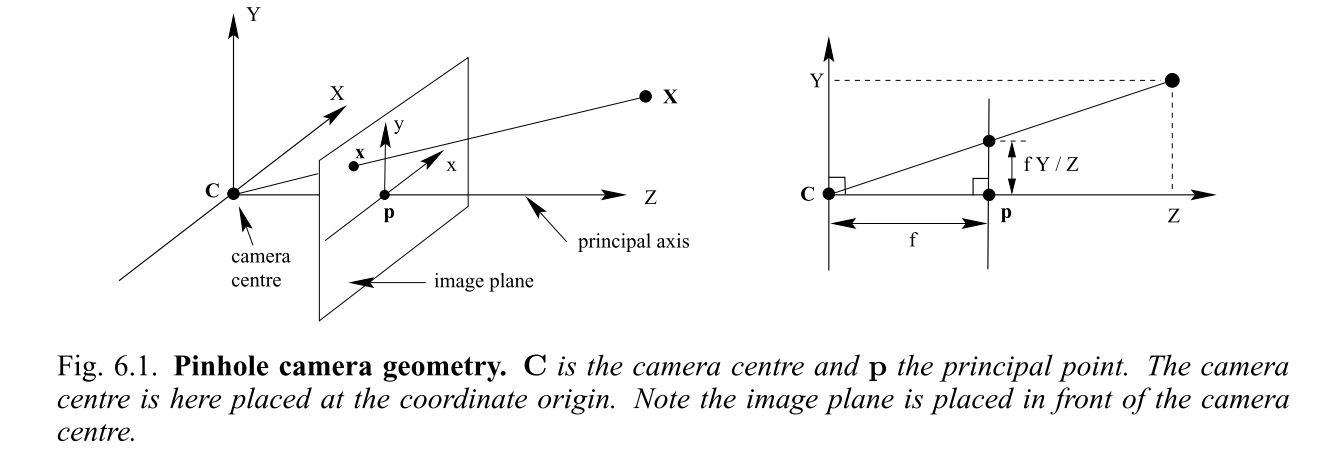
\includegraphics[width=\linewidth,natwidth=640,natheight=640]
  {fig/ref_imgs/pinhole_model.png}
  \caption{REMEMBER TO DRAW HORIZ/VERT Fx and Fy. The Pinhole Model}
	\label{fig:pinhole}
\end{figure}

Thanks to geometrical propotion property, we can project 
the 3D point $(X, Y, Z)^T$ in Euclidean space $\mathbb{R}^3$
to the 2D point $(U,V)^T = (f_xX/Z, f_yY/Z)^T$ in Euclidean space $\mathbb{R}^2$, 
where $f_x$ and $f_y$ are the \textit{focal lengths} 
between the camera centre and the pricipal 
point with respect to horizontal and vertical axis of the Camera Coordinate 
System respectively.
After projection, we obtain a 2D 
point that we represent on the 
\textit{Image Coordinate Frame} $(u_{img},v_{img})$.

To be more specific,
we can write the projection operation as a linear mapping function 
in the following way if we utilize the homogenous coordinates:

NOTE: NAME x,y,z indices for world and camera coords all below

\begin{equation}
  \begin{pmatrix}
    U\\
    V\\
    1
  \end{pmatrix}
  \sim
  Z
  \begin{pmatrix}
    f_xX/Z\\
    f_yY/Z\\
    1
  \end{pmatrix}
  =
  \begin{pmatrix}
    f_xX\\
    f_yY\\
    Z
  \end{pmatrix}
  =
  \begin{bmatrix}
    f_x & 0 & 0 & 0\\
    0 & f_y & 0 & 0\\
    0 & 0 & 1 & 0\\
  \end{bmatrix}
  \begin{pmatrix}
    X\\
    Y\\
    Z\\
    1
  \end{pmatrix}
\end{equation} \label{eq:proj_func_w_f}

This equation applies for the case when 3D points are 
projected onto a plane where the principal point is the origin. 
However, the common convention in partice 
is to have the origin at the (not entirely sure) left-bottom corner not in the centre.

\begin{figure}[H]
	\centering
	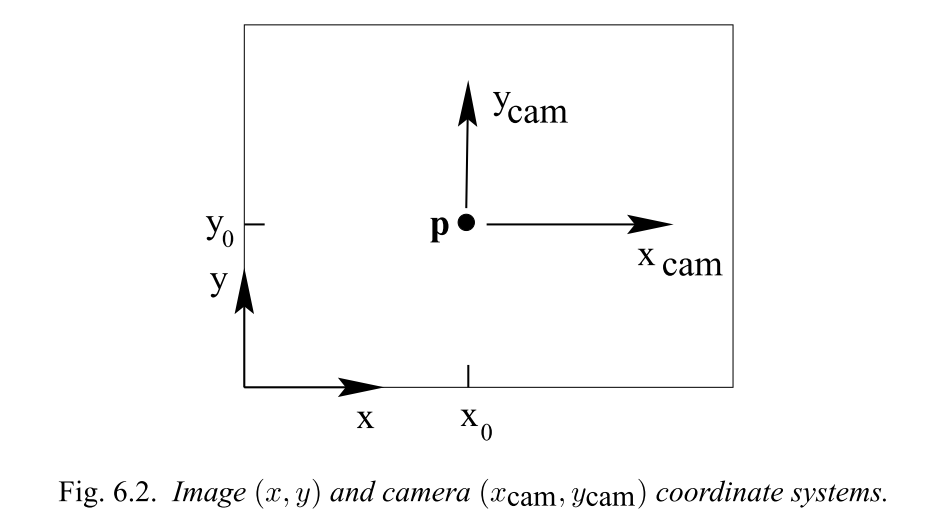
\includegraphics[width=\linewidth,natwidth=640,natheight=640]
  {fig/ref_imgs/pinhole_offset.png}
	\caption{Principle Point Offset}
	\label{fig:pinhole_offset}
\end{figure}

Thus, we get offsets, which can further be added into our function:

\begin{equation}
  \begin{pmatrix}
    U\\
    V\\
    1
  \end{pmatrix}
  \sim
  Z
  \begin{pmatrix}
    (f_xX + Z c_x)/Z\\
    (f_yY + Z c_y)/Z\\
    1
  \end{pmatrix}
  =
  \begin{pmatrix}
    f_xX + Z c_x\\
    f_yY + Z c_y\\
    Z
  \end{pmatrix}
  =
  \begin{bmatrix}
    f_x & 0 & c_x & 0\\
    0 & f_y & c_y & 0\\
    0 & 0 & 1 & 0\\
  \end{bmatrix}
  \begin{pmatrix}
    X\\
    Y\\
    Z\\
    1
  \end{pmatrix}
\end{equation} \label{eq:proj_func_w_f_c}

where $c_x$ and $c_y$ are coordinates of the principal point \textbf{p}.

In addition to pricipal offsets, inaccurately synchronized pixel-sampling 
process can result in \textit{skewed pixels}. This camera imperfection leads to 
non-square pixels as seen in Figure-\ref{fig:skewed}.

\begin{figure}[H]
	\centering
  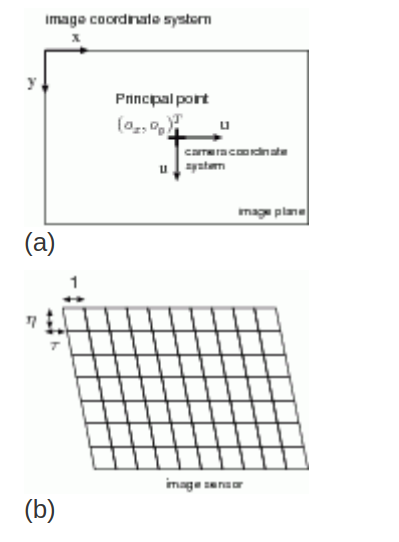
\includegraphics[width=0.5\linewidth,natwidth=640,natheight=640]
  {fig/ref_imgs/skew.png}
  \caption{REMEMBER TO DRAW FOR X and Y.Skew and Non-Square Pixels}
	\label{fig:skewed}
\end{figure}

We can scale the square pixels, having 1:1 pixel aspect ratio, with the 
corresponding skew parameters $\eta_x$, $\eta_y$ and $s$:

\begin{equation}
  \begin{pmatrix}
    U\\
    V\\
    1
  \end{pmatrix}
  \sim
  \begin{bmatrix}
    f_x\eta_x & s & c_x & 0\\
    0 & f_y\eta_y & c_y & 0\\
    0 & 0 & 1 & 0\\
  \end{bmatrix}
  \begin{pmatrix}
    X\\
    Y\\
    Z\\
    1
  \end{pmatrix}
  =
  \begin{bmatrix}
    \alpha_x & s & c_x & 0\\
    0 & \alpha_y & c_y & 0\\
    0 & 0 & 1 & 0\\
  \end{bmatrix}
  \begin{pmatrix}
    X\\
    Y\\
    Z\\
    1
  \end{pmatrix}
\end{equation} \label{eq:proj_func_w_square_pix_skew}

Generally, the skewed pixels issues occurred in ealier versions of CCD cameras 
and this is mostly fixed in new generation digital cameras. Therefore, 
we can neglate this effect by taking $\eta_x=1$, $\eta_y=1$ and $s=0$.

Next, we can extract:

\begin{equation}
  \mathbf{K} = 
  \begin{bmatrix}
    \alpha_x & s & c_x\\
    0 & \alpha_y & c_y\\
    0 & 0 & 1\\
  \end{bmatrix}
\end{equation} \label{eq:k_matrix}

The $\mathbf{K}$ matrix is called 
\textit{intrinsic parameters matrix}, which represents the characteristics of 
a camera sensor. Note that, we 
can further reformulate the notation \ref{eq:proj_func_w_square_pix_skew} in more 
compact form:

\begin{equation}
  \mathbf{x_{img}} = \mathbf{K}[\mathbf{I}|\mathbf{0}]\mathbf{X_{cam}}
\end{equation} \label{eq:simplyfied_proj_func}

\begin{figure}[H]
	\centering
  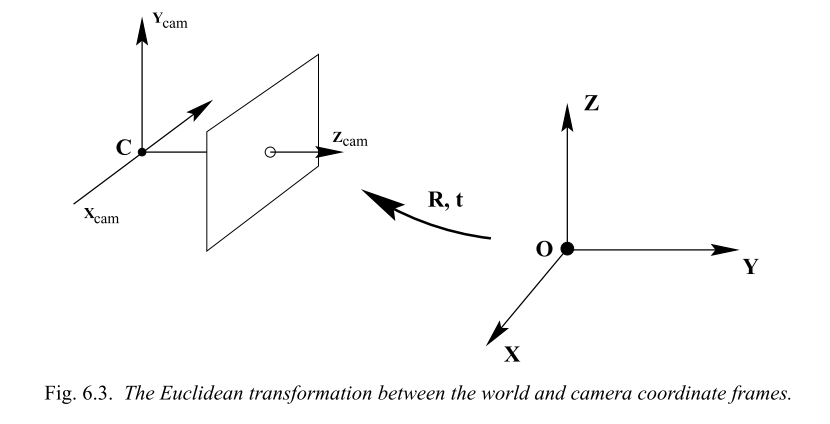
\includegraphics[width=\linewidth,natwidth=640,natheight=640]
  {fig/ref_imgs/cam_model_rot_trans.png}
  \caption{Camera Rotation and Translation}
  \label{fig:cam_model_rot_trans}
\end{figure}

Remember that, the Z-axis of the Camera Coordinate System aligns with the 
principal axis that is \textit{local} to camera frame. In fact, we have 3D points that 
we represent in the \textit{World Coordinate System} 
which we refer as the \textit{global} frame. 
These two coordinates systems 
can be transformed one another by a rotation and a translation as it is 
depicted in Figure-\ref{fig:cam_model_rot_trans} but we are interested in 
converting from the World Coordinate to Camera Coordinate System in this case.
To do so, we first perform series of rotations around each axis of the 
cartesian coordinate system in Euclidean space by using 
\textit{rotation matrices} where $R_x, R_y, R_z \in SO(3)$ is the rotation group:

\begin{equation}
  R_x(\theta) = 
  \begin{bmatrix}
    1 & 0 & 0\\
    0 & cos\theta & -sin\theta\\
    0 & sin\theta & cos\theta
  \end{bmatrix}
\end{equation} \label{eq:rot_matrx_x}

\begin{equation}
  R_y(\theta) = 
  \begin{bmatrix}
    cos\theta & 0 & -sin\theta\\
    0 & 1 & 0\\
    sin\theta & 0 & cos\theta
  \end{bmatrix}
\end{equation} \label{eq:rot_matrx_y}

\begin{equation}
  R_z(\theta) = 
  \begin{bmatrix}
    cos\theta & -sin\theta & 0\\
    sin\theta & cos\theta & 0\\
    0 & 0 & 1
  \end{bmatrix}
\end{equation} \label{eq:rot_matrx_z}

One can concatenate all three rotations about axes z, y, x respectively:

\begin{equation}
  \mathbf{R} = \mathbf{R_z(\gamma)}\mathbf{R_y(\beta)}\mathbf{R_x(\alpha)}
  =
  \begin{bmatrix}
    r_{11} & r_{12} & r_{13}\\
    r_{21} & r_{22} & r_{23}\\
    r_{31} & r_{32} & r_{33}\\
  \end{bmatrix}
\end{equation} \label{eq:rot_matrix_derivation}

Then, perform a translation $\mathbf{t} \in \R^{3x1}$:

\begin{equation}
  \mathbf{t} = 
  \begin{bmatrix}
    t_x \\ t_y \\ t_z
  \end{bmatrix}
\end{equation} \label{eq:translation}

We can also compound the rotation matrix and the translation vector into 
one matrix:

\begin{equation}
  \mathbf{T} =
  \begin{bmatrix}
    r_{11} & r_{12} & r_{13} & t_x\\
    r_{21} & r_{22} & r_{23} & t_y\\
    r_{31} & r_{32} & r_{33} & t_z\\
  \end{bmatrix}
\end{equation} \label{eq:transformation_matrix}

The $\mathbf{T} \in \R^{4x3}$ matrix in fact represents 
a \textit{rigid-body transformation}, which we call 
\textit{extrinsic camera parameters}.

Finally, we combine intrinsic $\mathbf{K}$ and 
extrinsic $\mathbf{T}$ matrices to form the following notation: 

\begin{equation}
  \mathbf{x_{img}} = 
  \mathbf{P}\mathbf{X_{world}} = 
  \mathbf{K}\mathbf{T}\mathbf{X_{world}} = 
  \mathbf{K}[\mathbf{R}|\mathbf{t}]\mathbf{X_{world}} =
  \mathbf{K}\mathbf{X_{cam}}
\end{equation} \label{eq:simplyfied_proj_func_1}

\begin{equation}
  \mathbf{x_{img}} = \mathbf{F_{proj}}(\mathbf{X_{world}})
\end{equation} \label{eq:simplyfied_proj_func_2}

where $\mathbf{F_{proj}}(\mathbf{X_{world}})$ is the 
\textit{projective transformation function}, which takes 
the 3D points in the World Coordinate System, transforms to 
the Camera Coordinate Systems and then maps them into the Image 
Coordinate Systems.

To build any reliable computer vision application with digital cameras, it is 
to important to find a good $\mathbf{P}$ \textit{projection matrix}. 
The next section describes one of many numerical methods for estimationg this 
matrix in literature.

\section{The Triangulation Model} \label{sc_depth_model}

Projected images captured by RGB cameras lack depth and angle 
information. To acquire these information, two main techniques are developed; 
e.g., passive stereo cameras and active stereo cameras. For passive stereo cameras, 
typically two synchronized cameras are placed horizontally with a known distance to each other. 
Hence, one usually exploits the triangulation technique to calculate the depth. 
Whereas, for active stereo camera, one typically has one light projector and 
one camera sensor. For example, in Kinect, a Infrared (IR) laser projects 
structured IR speckle light pattern on a object, and then 
the deformed light due to 3D geotmerty of the object are 
captured with a monochrome IR camera from different 
position (see figure-\ref{fig:kinect_depth_img}). 

\begin{figure}[H]
	\centering
  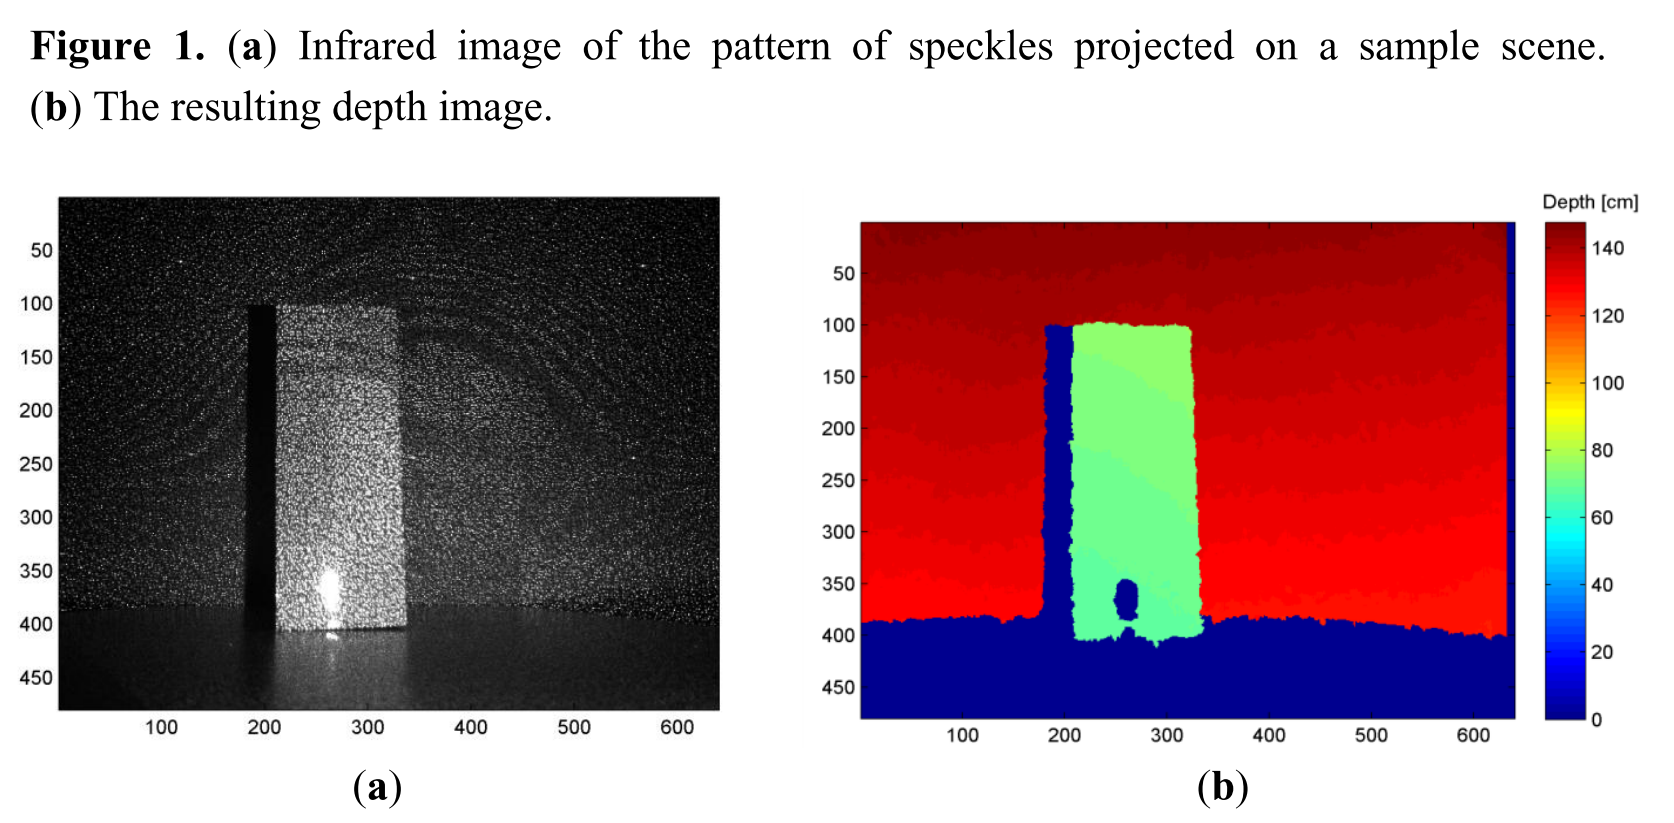
\includegraphics[width=0.7\linewidth,natwidth=640,natheight=640]
  {fig/ref_imgs/kinect_depth_img.png}
  \caption{Kinect Depth Image Construction}
	\label{fig:kinect_depth_img}
\end{figure}

Since we use Kinect in order to retrive depth information for our experiments, 
we will be modeling active stereo vision principle even though the 
basic principle behind them is the same mathematical model, which is 
the \textit{triangulation model}. This model is another geometrical model that 
takes advantages of similarity triangles to calculate the depth. 

\begin{figure}[H]
	\centering
  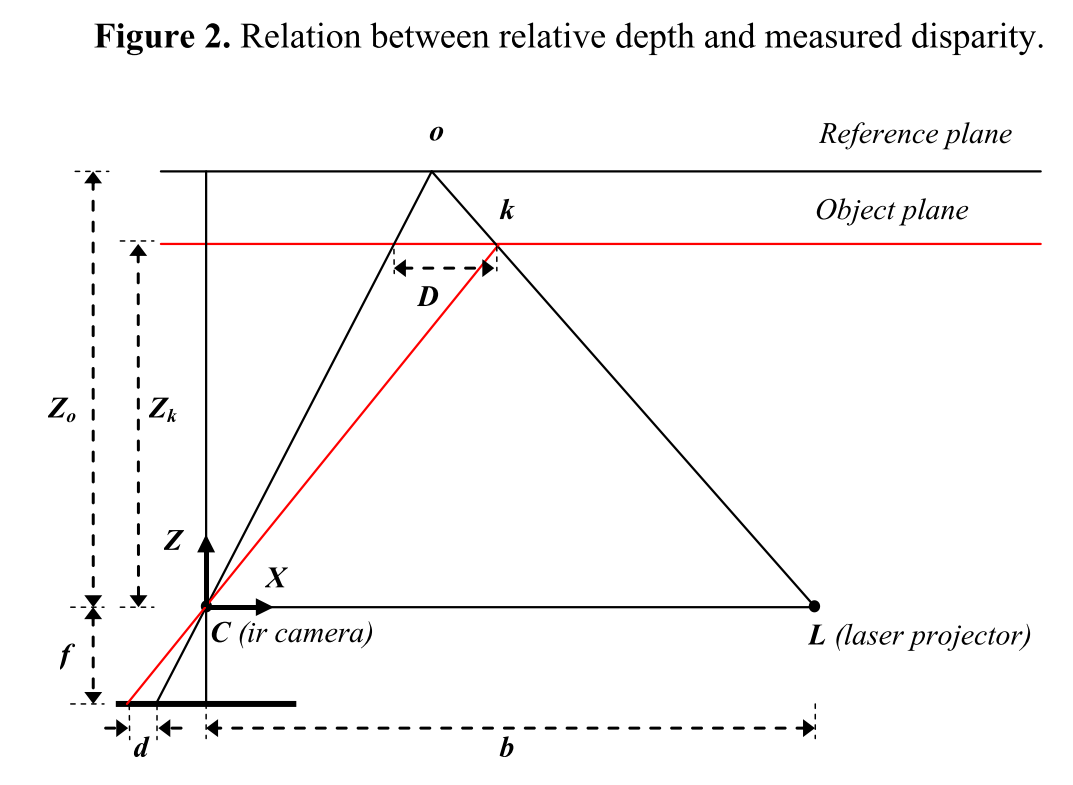
\includegraphics[width=0.7\linewidth,natwidth=640,natheight=640]
  {fig/ref_imgs/kinect_depth_measurement.png}
  \caption{Kinect's Depth Measurement}
	\label{fig:uncertainty_matching}
\end{figure}

In this setup, 
we again utilize the Camera Coordinate system similar to RGB camera
and IR camera with $f$ focal length is placed by facing perpendicular to 
the (principle axis) Z-axis at the origin. Then, IR laser projector is 
also placed along the X-axis parallel to the IR camera with $b$ distance. 
Additionally, we measure $d$ as a \textit{disparity} data and 
the maximum range that can be measured refers to $Z_r$. Ultimately, we are 
interested in finding $Z_i$ distance if depth information of point $k$ 
is desired. For doing so, we build two useful relationships using similarity of triangles:


\begin{equation}
  \frac{D}{b} = \frac{Z_r - Z_i}{Z_r} \text{ and } \frac{d}{f} = \frac{D}{Z_i}
\end{equation}

If the depth camera paramters such as $(f, b, Z_r)$ is 
calibrated and we measure $d$ disparity data, 
we can easily extract $Z_i$ depth information with the following formula:

\begin{equation}
  Z_i = \frac{Z_r}{1+\frac{Z_r}{fb}d}
\end{equation}\label{eq:depth_wo_disparity}

Another important point to note is that Kinect or other depth cameras in pratice might 
not provide the depth metric information directly. For instance, 
Kinect provides us disparity image data that correspond to inverse depth 
quantized with 11 bits and the relationship between disparity data and 
real depth is non-linear as shown in \ref{fig:depth_disparity_relation}.

\begin{figure}[H]
	\centering
  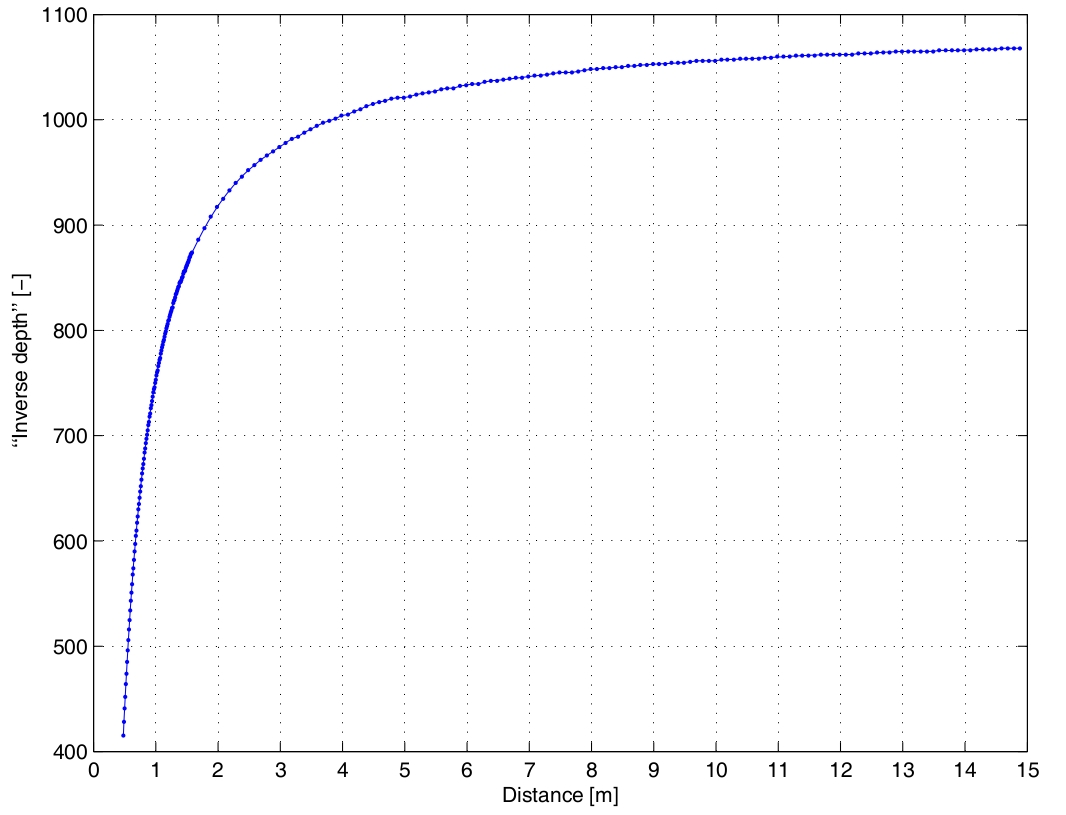
\includegraphics[width=0.7\linewidth,natwidth=640,natheight=640]
  {fig/ref_imgs/depth_disparity_relation.png}
  \caption{Inverse Depth and Disparity Data Relationship}
	\label{fig:depth_disparity_relation}
\end{figure}

Thus, we need to update depth equation \ref{eq:depth_wo_disparity} by 
taking its inverse and 
introducing denormalization factor replacing with $d$ with $md'+n$:

\begin{equation}
  Z_i^{-1} = (\frac{m}{fb})d' + (Z_r^{-1} + \frac{n}{fb})
\end{equation}\label{eq:depth_w_disparity_reverse}

To make it convenient to calculate, we can take its inverse again:

\begin{equation}
  Z_i = \frac{1}{(\frac{m}{fb})d' + (Z_r^{-1} + \frac{n}{fb})}
\end{equation}\label{eq:depth_w_disparity}

Now that we know how to get metric depth information $Z_i$ from disparity data by 
utilizing the triangulation model, we can discuss 
how
$X_i$ and $Y_i$ 
coordinates of the point $\mathbf{X_{world}}=[X_i, Y_i, Z_i]^T$ in World Coordinate System
are projected as $\mathbf{x_{img}}=[u_k,v_k,1]^T$ pixel coordinates of the IR camera. 
To do so, we require the similar projection function to RGB camera 
(see section \ref{sb_sc_pinhole})
consists of intrinsic and extrinsic camera parameters, but this time it is for 
the IR camera:

\begin{equation}
  \mathbf{X_{world}} =
  Z_i (\mathbf{P_{IR}^{-1}}\mathbf{X_{world}}) = 
  Z_i (\mathbf{K_{IR}^{-1}}\mathbf{T_{IR}^{-1}}\mathbf{x_{img}})
\end{equation} \label{eq:ir_cam_proj_func}


%One can also retrive remaining $X_k$ and $Y_k$ coordinates of point $k$ in the Camera 
%Coordinate system if coordinates of the principal point $(c_x, c_y)$ of the 
%IR camera and its distortion paramaters $(\delta x, \delta y)$ are calibrated, and 
%$u_k$ and $v_k$ coordinates of the point $k$ in the image plane is measured:
%
%\begin{equation}
%\begin{aligned}
%  X_k = -\frac{Z_k}{f} (u_k - c_x + \delta x)\\
%  Y_k = -\frac{Z_k}{f} (v_k - c_y + \delta y)
%\end{aligned}
%\end{equation}

To find related intrinsic parameters for RGB and depth camera, we will perform 
calibration process in the following section.

\section{RGB-D Camera Calibration} \label{sb_sc_rgb_calibration}

The calibration process is a crucial part of any computer vision applications 
and there are many sophisticated techniques to achieve accurately.
However, it is important to note that full derivations of the calibration formulation 
is not provided, but only the important points are given.
Therefore, I refer readers to \cite{bla} for the rgb camera calibration and 
to \cite{bla} for the depth camera calibration. 
Since we are about to calibrate two cameras; i.e., RGB and depth, that we 
used to register each 3D point cloud with a color, we assume that both camera's image 
planes are aligned and it has 1:1 pixel correspondences. Under this assumption,
let's start with RGB camera.

\subsubsection{RGB Camera}

Assuming that we project two 3D points onto our image plane
like in Figure-\ref{fig:calibration_constraint},
the visual angle between those pair of 3D points is equal to 
the angle between its corresponding 2D points. This geometric constraints 
allow us to build the calibration problem. Remember that the goal is to find 
the projection matrix and we can build the problem in the following way:

\begin{figure}[H]
	\centering
  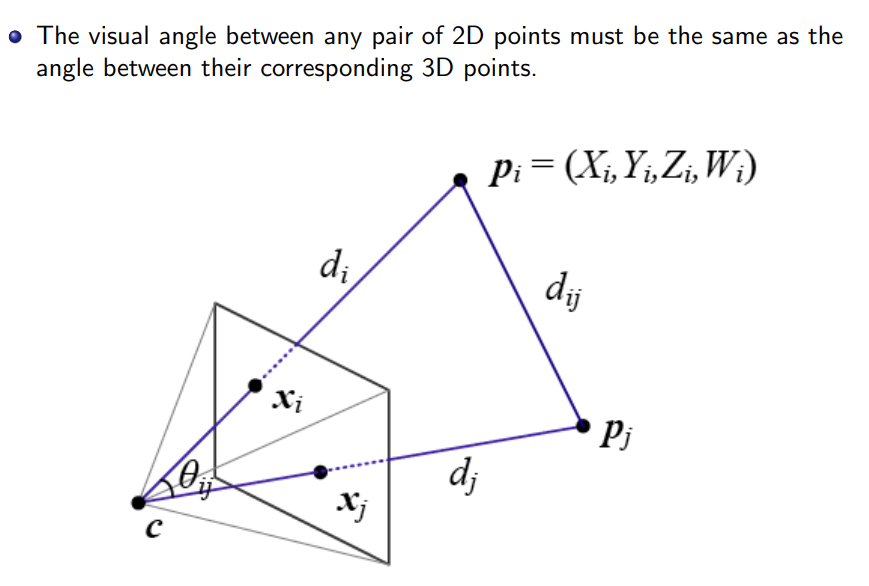
\includegraphics[width=\linewidth,natwidth=640,natheight=640]
  {fig/ref_imgs/calibration_dlt.png}
  \caption{Inherit Constraint}
  \label{fig:calibration_constraint}
\end{figure}


\begin{equation}
  \mathbf{x_{img}} = 
  \begin{pmatrix}
    u_i\\
    v_i\\
    1
  \end{pmatrix}
  =
  \mathbf{P}\mathbf{X_{world}} = 
  \begin{bmatrix}
    p_{00} & p_{01} & p_{02} & p_{03}\\
    p_{10} & p_{11} & p_{12} & p_{13}\\
    p_{20} & p_{21} & p_{22} & p_{23}
  \end{bmatrix}
  \begin{pmatrix}
    X_i\\
    Y_i\\
    Z_i\\
  \end{pmatrix}
\end{equation} \label{eq:proj_matrix}

Let's now distribute 
the projection matrix onto the 3D point measurement to retrieve individual 
pixel coordinates:

\begin{equation}
  u_i = 
  \frac
  {p_{00}X_i + p_{01}Y_i + p_{02}Z_i + p_{03}}
  {p_{20}X_i + p_{21}Y_i + p_{22}Z_i + p_{23}}
\end{equation} \label{eq:u_i}

\begin{equation}
  v_i = 
  \frac
  {p_{10}X_i + p_{11}Y_i + p_{12}Z_i + p_{13}}
  {p_{20}X_i + p_{21}Y_i + p_{22}Z_i + p_{23}}
\end{equation} \label{eq:v_i}


Since $\mathbf{x_{img}}$ and $\mathbf{X_{world}}$ are known,
we can find elements of the $\mathbf{p} = (p_{00}, p_{01}, \dots, p_{23})^T$ matrix 
by solving $\mathbf{Ap=0}$ liner system of equations from \ref{eq:u_i} and \ref{eq:v_i}.

For \textit{minimal solution} of this linear system of equations, 
we need at least $n \geq 6$ measurement points to solve the problem as 
the $\mathbf{P}$ matrix has 12 degree of freedom (11 if scale is ignored).
Note that this accounts for having 
noise-free measurement which does not hold in reality. Then, the problem 
becomes \textit{over-determined}.

In noisy measurement case, the problem is usually solved with
\textit{singular value decomposition (SVD)} with $n \geq 6$ measurement points. 
This method is called the \textit{Direct Linear Transformation (DLT)}.
Disadvantange of the DLT methods, it is still sensitive errors since 
it only considers \textit{algebraic errors}, which are the residuals of 
$\mathbf{Ap}$. 

While estimating the intrinsic and extrinsic parameters 
that are in linear form with the DLT, 
another issue known as \textit{radial distortion} 
has to take into account as well. This issue is caused by camera lens 
and Figure-\ref{fig:cam_distortion} depicts this effect and the straight lines 
appear to be curved. 

\begin{figure}[H]
	\centering
  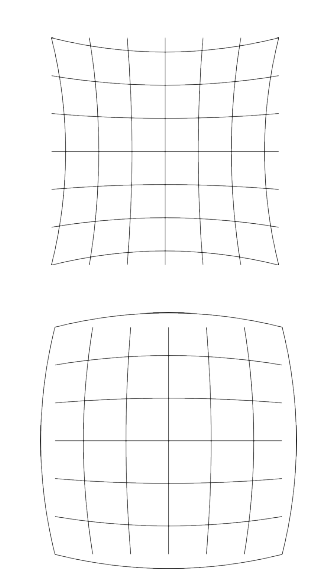
\includegraphics[width=0.3\linewidth,natwidth=640,natheight=640]
  {fig/ref_imgs/cam_distortion.png}
  \caption{Camera Distortion}
  \label{fig:cam_distortion}
\end{figure}

This distortion has non-linear characteristics and we also 
need to estimate the coefficients 
$\kappa = (k_1, k_2, p_1, p_2, k_3)^T$ of the following polynomial:


\begin{equation}
\begin{split}
  x''_i = F_{dist}(x') = 
  x'(1+ k_1 r^2 + k_2 r^4 + k_3 r^6) + 2 p_1 x' y' + p_2 (r^2+2x'^2)\\
  y''_i = F_{dist}(y') = 
  y'(1+ k_1 r^2 + k_2 r^4 + k_3 r^6) + p_1 (r^2+2y'^2) + 2p_2 x'y'\\
\end{split}
\end{equation}

where $x' = X_{cam}/Z_{cam}$ and $y' = Y_{cam}/Z_{cam}$. 
Note that, in \ref{eq:simplyfied_proj_func}, we first transform 
3D points from World Coordinate to Camera Coordinate Systems with 
extrinsic matrix and then we project them with the instrinsic matrix. 
To improve our pinhole camera model, 
we need to distort 3D points in the Camera Coordinate System before 
multiplying with the intrinsic matrix:

\begin{equation}
  \begin{pmatrix}
    U\\
    V\\
    1
  \end{pmatrix}
  =
  \begin{pmatrix}
    f_x x'' + c_x\\
    f_y y'' + c_y\\
    1
  \end{pmatrix}
    =
    F_{dist}\begin{pmatrix}
      \mathbf{K}
      \begin{pmatrix}
        X_{cam}\\
        Y_{cam}\\
        Z_{cam}\\
        1
      \end{pmatrix}
    \end{pmatrix} 
    =
    F_{dist}\begin{pmatrix}
      \mathbf{K} [\mathbf{R}|\mathbf{t}]
      \begin{pmatrix}
        X_{world}\\
        Y_{world}\\
        Z_{world}\\
        1
      \end{pmatrix}
    \end{pmatrix}
\end{equation} \label{eq:proj_func_w_f_c}

Above operations introduce non-linearity, which cannot be solved by DLT.
To get better accuracy at our projection matrix along with the distortion, 
\textit{least squares estimation}, i.e., Levenberg-Marquardt, is perfomed.

\begin{figure}[H]
	\centering
  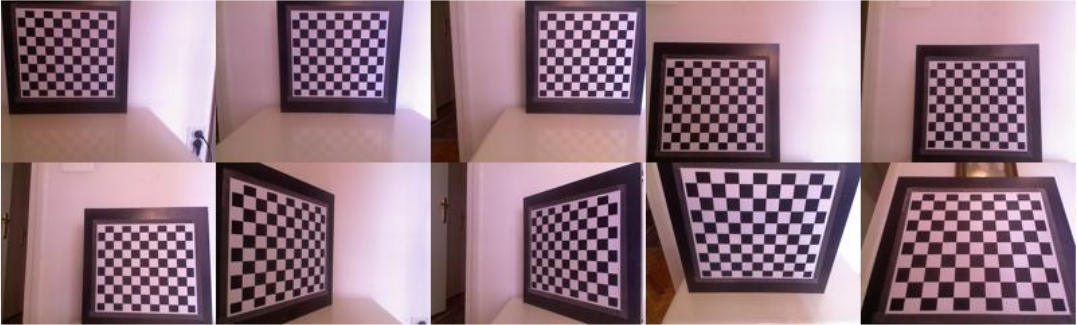
\includegraphics[width=0.5\linewidth,natwidth=640,natheight=640]
  {fig/ref_imgs/checkerboard_rgb.png}
  \caption{Checkerboard RGB}
  \label{fig:checkerboard_rgb}
\end{figure}

In practice, the checkerboard is used to get many good measurement points 
as  we easily extract edge features from the image. Now, the DLT comes handy
as we can use the DLT's result as an initial guess 
in the least squares optimization problem.

\begin{equation}
  \argmin_{\mathbf{P_{RGB}} \rightarrow \mathbf{K_{RGB}}, \kappa_{RGB}, \mathbf{R_{RGB}}^{(i)}, \mathbf{t_{RGB}}^{(i)}}
  \sum_{i=1:n} || \mathbf{x_{img}}^{(i)} - 
  \mathbf{P_{RGB}} \mathbf{X_{world}}^{(i)} ||^2
\end{equation}\label{eq:proj_lsq}

where we use known 
$\mathbf{x}_i$ is the pixel coordinates of a feature on image plane and 
$\mathbf{X}_i$ is the coordinates of a feature in World Coordinate system
to identify the following parameters:

\begin{itemize}
  \item $\mathbf{K_{RGB}}$ is the intrinsic matrix for RGB camera, 
  \item $\kappa_{RGB}$ is the distortion coefficients for RGB camera, 
  \item $\mathbf{R_{RGB}}^{(i)}$ is the corresponding orientation for RGB camera and 
  \item $\mathbf{t_{RGB}}^{(i)}$ is the corresponding translation for RGB camera.
\end{itemize}

\subsubsection{Depth Camera}

The depth camera almost has an identical procedure to RGB camera with minor 
differences. 
To begin with the calibration process, 
we, similarly, capture the depth image of checkerboard at the same position 
with RGB camera and detect the same features as shown in the following figure.

\begin{figure}[H]
	\centering
  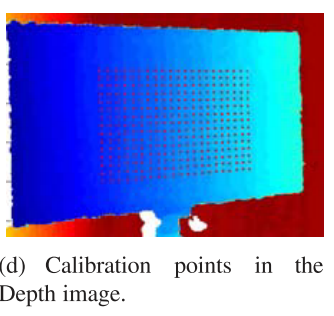
\includegraphics[width=0.5\linewidth,natwidth=640,natheight=640]
  {fig/ref_imgs/checkerboard_depth.png}
  \caption{Checkerboard Depth}
  \label{fig:checkerboard_depth}
\end{figure}

The difference is, however, in the cost fuction of least squares equation. 
For RGB camera, we minimize the error on the image plane (see \ref{eq:proj_lsq}) 
by projecting 3D points in world onto image plane. Whereas, for depth camera, 
we will minimize the error in the World Coordinate system since we need to 
include depth $Z_i$ into the calibration process (remember \ref{eq:depth_w_disparity}).


\begin{equation}
  \argmin_{\mathbf{P_{IR}} \rightarrow \mathbf{K_{IR}}, \kappa_{IR}, \mathbf{R_{IR}}^{(i)}, \mathbf{t_{IR}}^{(i)}}
  \sum_{i=1:n} || \mathbf{X_{world}}^{(i)} - 
  Z_i (\mathbf{P_{IR}^{-1}} \mathbf{x_{img}}^{(i)}) ||^2
\end{equation}\label{eq:proj_lsq}

where we use known 
$\mathbf{x_{img}}^{(i)}$ is the pixel coordinates of the same feature on image plane and 
$\mathbf{X_{world}}^{(i)}$ is the coordinates of the same feature in World Coordinate system
to identify the following parameters:

\begin{itemize}
  \item $\mathbf{K_{IR}}$ is the intrinsic matrix for IR camera, 
  \item $\kappa_{IR}$ is the distortion coefficients for IR camera, 
  \item $\mathbf{R_{IR}}^{(i)}$ is the corresponding orientation for IR camera and 
  \item $\mathbf{t_{IR}}^{(i)}$ is the corresponding translation for IR camera.
\end{itemize}


The afromentioned calibration processes are well-studied problem in 
computer vision literature. 
Fortunately, there are many software libraries, such as OpenCV, 
that offers such implementations.


\chapter{Fundamentals of Visual Odometry} \label{cp_vo}

\section{Related Works} \label{sc_visual_odometry_related_works}

% First ego motion estimation with cam
% - Moravec1980 - Obstacle Avoidance and Navigatio n in the Real World by a Seeing Robot Rover
% - Matthies1987a - Error Modeling in Stereo Navigation
% - Olson2003 - Rover navigation using stereo ego-motion
First research in estimating camera ego-motion was done in 
a PhD Thesis \cite{Moravec1980} in 1980s. He used a sliding camera as 
a stereo fashion that captures images when the robot stopped after moving for some 
small distance. Another early study, from Matthies and Shafer \cite{Matthies1987a}, 
formulized the ego-motion estimation for stereo vison.
The interest in VO peaked 
after NASA's Mars expeditions with a rover in 2003 . 
Reseachers and engineers in NASA JPL further improved the robutness of 
their robots since it was a critical application \cite{Olson2003}.
% First VO Paper
% Nister2004 - Visual Odometry

For the first time, Visual Odometry term was introduced in \cite{Nister2004} 
by the computer vision researchers. 
It estimates the transformation matrix by solving the P3P problem between consecutive frames.
Nister also demonstrated a VO pipeline that became a defacto system configuration even 
for today's VO applications.
In computer vision, Structure from Motion (SFM), that tackles 3D reconstruction of 
an environment with moving camera, is well-studied topic. For SFM, it is critical 
to estimate camera pose accurately to build the 3D environment. VO 
can be thought of subset problem of SFM. 
The reason VO parted from SFM is 
because VO systems started to empower other applications such SLAM and 
are required to operate in real-time, all of which introduces 
a great challenge. With the help of early robotics applications 
in NASA and computer vision community, the VO became quite popular field. 
That being said, two of the most influential papers were 
\cite{Fraundorfer2012} and \cite{Scaramuzza2011}. By publishing these tutorials, 
the authors gave researchers and engineers a design recipe for building the 
right VO system since there is no such a system that works under any conditions.
One can also find a survey of VO types, approaches and challenges in 
\cite{Aqel2016}.
% Surveys
% - Fraundorfer2012 - Visual odometry: Part I: The First 30 Years and Fundamentals
% - Scaramuzza2011 - Visual Odometry Part II: Matching,Robustness, Optimization, and Applications
% - Aqel2016 - Review of visual odometry: types, approaches, challenges, and applications

Over the years, research on VO is progressively increased and various types of 
VO systems are proposed. Therefore, 
VO systems can be categorized based on different phenomenas such as 
camera sensor types and solver algorithms choice.
One can utilize monucular or stereo cameras in order to capture images. 
The stereo cameras are further grouped 
into two category; i.e., active and passive cameras. For active camera, 
besides color or monochrome camera, there is another camera such IR camera that measures the depth information. 
For passive camera, the depth is calculated from two color or monochrome camera. 
In the case of solver algorithms, one can group VO into two category; i.e.,
feature-based and appearance-based.

The feature-based VO algorithms are interested in extracting distinct and  
repeatable feature points from images and finding correspondences in 
extracted features either between consecutive frames or keyframes. 
Before estimating camera poses, 
an important step for the feature-based alogrithms is to remove outliers 
in feature matches with RANSAC \cite{Fischler1981}
% Fischler1981 - RANSAC
There are two popular open source feature-based VO tools; i.e., 
LIBVISO2 \cite{Geiger2011} and FOVIS \cite{Huanga2011}.
To explain LIBVISO2 briefly, 
both simple blob and corner filters are used to extract features.
The extracted features are filtered by non-maximum suppression to increase 
the robustness of the matching process.
Then, it calculates the depth information by triangulation technique as 
it uses passive stereo camera. Finally, they minimize the reprojection error. 
The reprojection error function is constructed by projection from 
features on the left camera onto the right camera and vice-versa, 
to estimate the pose. Note that RANSAC applied on feature matches to remove 
outliers. On the other hand, FOVIS is more accurate and faster than 
LIBVISO2 according to \cite{Fang2015a}.
% RGBD VO Comparisons
%% - Angladon2017 - An evaluation of real-time RGB-D visual odometry algorithms on mobile devices
% - Fang2015a - Experimental evaluation of RGB-D visual odometry methods
FOVIS uses only FAST corner detectors to extract features. 
For the matchings, FOVIS uses keyframe fashion instead of consective images to 
reduce the drift.
Instead of 
using RANSAC for outlier rejection, it contructs 
a graph of consistent feature matches and updates the features that obey the 
idea that 
the Euclidean distance between two features at one time should match 
their distance at another time. Finally, several refinement processes are applied 
during motion estimation to improve accuracy.
% RGBD VO Implementations
% - Geiger2011 - LIBVISO2 - StereoScan: Dense 3d Reconstruction in Real-time
% - Huanga2011 - FOVIS - Visual Odometry and Mapping for Autonomous Flight Using an RGB-D Camera

The biggest disadvantage of feature-based VO is that accuracy of the pose estimations 
decreases if the operating environment lacks texture-rich scenes such as 
corridors or the measured images are blurry due to fast motions. Thus, 
appearance-based VO algorithms utilize the entire image instead of extracted features.
Initially, Iterative Closest Point (ICP) \cite{Besl1992} 
was used to minimize the geometrical error between 3D surfaces. There are 
also various kinds of ICP algorithms 
that offers to compute efficiently \cite{Rusinkiewicz2001}. Even though ICP 
is useful for creating 3D shapes with point clouds, it is slower and less 
accurate comparing to feature-based methods.
% - Besl1992 - First ICP Paper - A method for registration of 3-D shapes
% - Rusinkiewicz2001 - ICP - Efficient Variants of the ICP Algorithm
Then, another type of apperance-based approach, so-called Dense Visual Odometry (DVO) 
\cite{Kerl2013a}, 
was emerged by minimizing 
the photometrical error based on the pixel intensity between consecutive frames. 
% - Kerl2013a - DVO - Robust Odometry Estimation for RGB-D Cameras

%% - Dryanovski2013 - CCNY - Fast Visual Odometry and Mapping from RGB-D Data
%% - Fang2015a - DEMO - Real-time Depth Enhanced Monocular Odometry

TODO: OUTLINE THE FOLLOWING SECTIONS. DESCRIBE VO PIPELINE BRIEFLY.


\section{Feature Extraction} \label{sc_feature_extraction}

Image features are a collection of regions of interest or of points of interest 
that describe the image. In this way, we compress the necessary information 
from images so that we can achieve computationaly expensive task more efficiently.
Points of interest, also called \textit{keypoints}, 
are particularly valuable because their location in the image can be 
measured accurately. This is useful for localization related tasks such as VO. 

In feature-based VO, the critical task is to find good features. 
What defines a good feature from others is that it is distinct, 
repeatable, computationaly cheap and invariant to geometrical changes. 
Obviously, one has many options to produce such image 
feautes but two common methods that are widely used in VO systems are 
blobs and corners. 
Blobs are image patterns that contain distinct image response comparing to their 
neighborhood pixels. Blobs take advantage of pixel intensity or color to 
decide whether it has a distinct response or not.
In the VO literature, SIFT\cite{}, SURF\cite{} or CENSURE\cite{} are popular 
choices for detecting blob featurus.
Corners are the meeting points where two or many edges intersect. Corners, 
on the other hand, 
take advantage of geometrical structure of an image. FAST\cite{}, Shi-Tomasi or 
Haris\cite{} are widely used for detecting corners.

Fundemantally, a two-step process is needed to extract good features. 
First, you take a response function called \textit{image filter}, 
shift this filter through the image and save the one that have greater 
response than your previously defined threshold as Keypoints. 
This might a Gaussian filter for blobs or a 
corner detector filter for corners. In the second step (optional), 
you perform non-maxima 
suppression on the resulting keypoints to find local minima of the function. 
This step will help to remove similar keypoints and to choose the ones having 
maximum confidence so that distinctiveness of the features are ensured.

Inheritly, each feature detector has certain limitations and one has to 
choose which detector to use depending on task objectives. Therefore, we may ask 
the following question: 
Does the localization envorinment involve more texture oriented objects like 
floors, walls etc. or geometrical shapes like urban areas where many lines 
exist?
However, rule of thumb when choosing feature detector is that blobs 
are distinct but slow to compute and corners are fast to compute but less 
distict. 

%\subsection{Feature Descriptor} \label{sb_sc_feature_descriptor}

Extracting features is the very first step of VO. The next step is to 
encode the detected keypoints into a format that we can perform comparison 
or search operation among them. This is done by taking the neighboring pixels 
around the keypoints and convert into a more compact form. For example, SIFT 
, most well-known feature decsriptor, 
creates a patch around a keypoint, divides this patch into smaller grids,
calculate the gradient of each grid and 
saves them as a histogram.
This procedure makes feature descriptor 
robust agaist scale or rotation changes. Then, one can use these descriptors for 
various comparison operations such as matching or tracking in VO. However, we 
utilize the ORB in our VO and will discuss its properties.


\subsubsection{ORB} \label{sb_sc_orb}

One of the most strict requirements of VO is the real-time contraints since it is 
expected to work at similar to low-level inertial sensors, i.e., accelerometer, gyroscopes etc. 
As previously discussed, blobs detectors are computationaly expensive. Therefore, 
corners based feature detector are more prevelant in VO. 
\textit{ORB (oriented FAST and rotated BRIEF)} studied known issues of 
FAST detector and BRIEF descriptor. Then, it combines them to compansate each 
other's drawbacks. In the end,
it perform as accurate as SIFT, plus faster. Here are steps on how to extract features 
and create descriptors with ORB: 

\begin{enumerate}
  \item \textbf{Detect corners with FAST}: FAST take each pixel on 
    the image and compare with its adjacent pixels. More specificially, 
    ORB uses FAST-9, which takes a patch of discrete circular radius of $r=9$. 

    \begin{figure}[H]
	\centering
  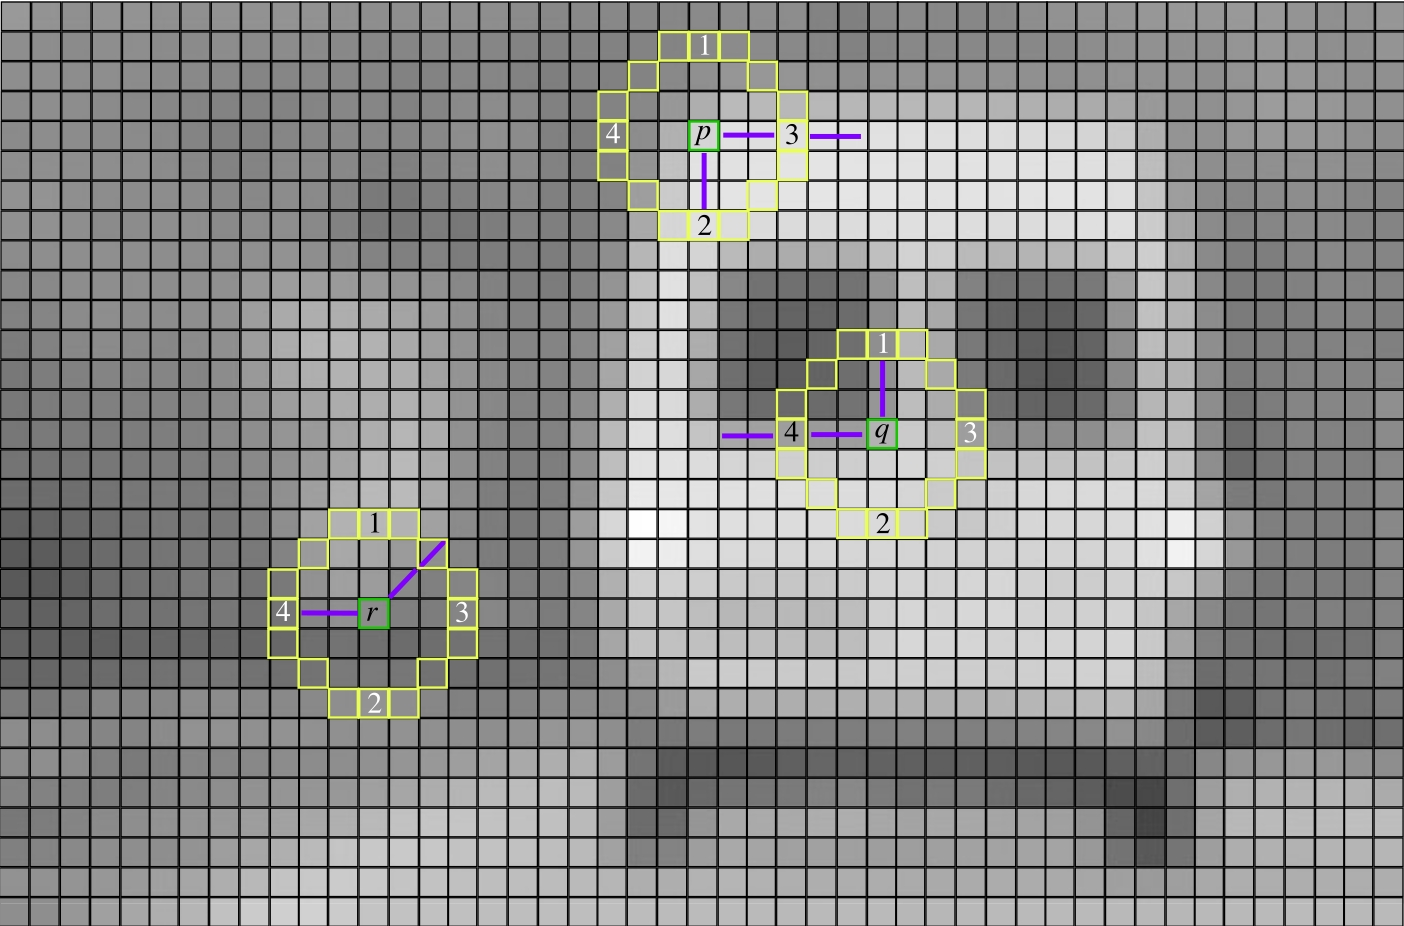
\includegraphics[width=0.6\linewidth,natwidth=640,natheight=640]
  {fig/ref_imgs/fast.png}
  \caption{FAST corners}
  \label{fig:fast_corners}
\end{figure}

    If the 
    selected pixel is $\pm t$ darker or brighter than adjacent pixels, 
    we call it a corner, where $t$ is our empiric threshold.

\begin{equation}
  M_c(p) = 
  \sum_{r \in S_{bright}} |I_{p \rightarrow r} - I_p| - t \text{ or } 
  M_c(p) = 
  \sum_{r \in S_{dark}} |I_p - I_{p \rightarrow r}| - t)
\end{equation}
    We retrieve $M^c_{1:n}$ the set of corner candidates from 
    comparing $I_{p\rightarrow x}$ the adjacent pixels around $I_p$ the target pixel.

  \item \textbf{Rank detected keypoint with Harris}: After FAST detection, 
    we get many corner candidates around the interest point. However, 
    FAST does not measure how good a corner is. Thus, we use Harris corner 
    detector to rank corner candidates:
    \begin{equation}
      \mathbf{A} = \sum_{x,y} w(x,y) 
      \begin{bmatrix}
        I_x^2 & I_xI_y \\ I_xI_y & I_y^2
      \end{bmatrix}
    \end{equation}
    The $\mathbf{A}$ matrix is calculated by the $I_x$ and $I_y$ partial 
    derivatives with respect to x and y direction and $w(x,y)$ weighting window.

    \begin{equation}
      R^c = det(\mathbf{A}) - k(trace(\mathbf{A}))^2
    \end{equation}
    where $det(\mathbf{A}) = \lambda_1 \lambda_2$ and 
    $trace(\mathbf{A}) = \lambda_1 + \lambda_2$.
    Then, we use the resulting $\mathbf{A}$ to find a ranking score for each 
    corner. Now, it is possible to take top N corners if desired.

  \item \textbf{Calculate orientation of corners with image moments}: 
    ORB uses BRIEF to create feature descriptors; however, BRIEF fails in 
    rotated images. Therefore, ORB modifies the BRIEF by adding orientation 
    information. To get orientation, an \textit{image moment} are calculated
    for each patch $\mathbf{S_n}$:

    \begin{equation}
      m_{a,b}(\mathbf{S_n}) = \sum_{x,y \in \mathbf{S_n}} x^a y^b I(x,y)
    \end{equation}
    where $a + b$ defines the order of the moment and we need 
    the moments of order one:

    \begin{equation}
      m_{1,0}(\mathbf{S_n}) = \sum_{x,y \in \mathbf{S_n}} x \cdot I(x,y) \text{  ,  }
      m_{0,1}(\mathbf{S_n}) = \sum_{x,y \in \mathbf{S_n}} y \cdot I(x,y)
    \end{equation}

    Then, we get the orientation of the patch $\mathbf{S_n}$:
    \begin{equation}
      \theta(\mathbf{S_n}) = atan2(m_{01}, m_{10})
    \end{equation}

  \item \textbf{Form BRIEF descriptors with their corresponding orientation}:
    Once the top N corners and their orientations are detected, descriptions 
    can be formed with BRIEF. 

\begin{figure}[H]
	\centering
  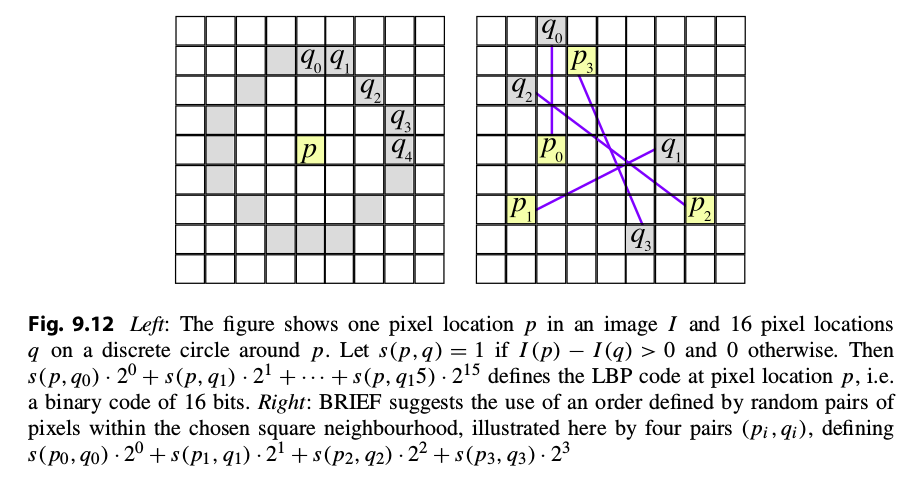
\includegraphics[width=\linewidth,natwidth=640,natheight=640]
  {fig/ref_imgs/brief.png}
  \caption{BRIEF pairs}
  \label{fig:brief_pairs}
\end{figure}


    To do so, we randomly (normal distribution) 
    selected 256 pairs $(p_i,q_i)$ 
    inside the patch $\mathbf{S_n}$:
    \begin{equation}
      \mathbf{S_n} = 
      \begin{pmatrix}
      p_0, \dots, p_n\\
      q_0, \dots, q_n
      \end{pmatrix}
    \end{equation}
    Next, we rotate each $(\mathbf{p_i, q_i})$ pair points in 
    $\mathbf{S_n}$ with the 
    corresponding corner's orientation:
    \begin{equation}
      \mathbf{p}_{i,\theta} = \mathbf{R}_{\theta}\mathbf{p_i} \text{ and } 
      \mathbf{q}_{i,\theta} = \mathbf{R}_{\theta}\mathbf{q_i}
    \end{equation}
    where $p_i=(x_i, y_i)$ and $q_i=(x_i, y_i)$ are the pixel coordinates of 
    the points.
    It is important to note that authors \cite{} suggested to rotate each point in 
    increments of 2$\pi$/30. Therefore, orientaion $\theta$ is mapped to 
    nearest multiple of 2$\pi$/30.

    To form steered (or rotated) BRIEF descriptors, we perform pixel density comparison:
    between randomly selected pair points:
    \begin{equation*}
      \tau(\mathbf{p_{i,\theta}},\mathbf{q_{i,\theta}}) := 
      \begin{cases}
        1  & I(\mathbf{p_{i,\theta}}) < I(\mathbf{q_{i,\theta}}),\\
        0  & I(\mathbf{p_{i,\theta}}) \geq I(\mathbf{q_{i,\theta}})
      \end{cases}
    \end{equation*}

    Finally, we sum comparison results with binary form to get the desctriptor 
    of the patch $\mathbf{S_n}$:
    \begin{equation}
      \mathbf{D_n} = f(\mathbf{S_n}) := \sum_{1\leq i \leq n} 2^{i-1}\tau (\mathbf{p_{i,\theta}, q_{i,\theta}})
    \end{equation}

\end{enumerate}





\section{Feature Matching} \label{sc_feature_matching}

Now that we know how to extract a distinct feature and to form a descriptor, 
we can start building a relationship across images to estimate how the camera 
moves. Remember that 
the camera can procedure
a video stream consisting of usually ranging from 30 to 60 frames per second. 
The first task is to form a group of image pairs and to compute translation and rotation 
information between each image pair, continuously. In literature, there are two ways to 
select image pairs: 
frame to frame or key frame to frame. In the former case, one pairs consecutive 
frames across video stream. In the latter case, one selects a reference 
frame and keep matching it with subsequent frames as long as the pair has 
sufficient amount of feature matchings. The latter has certain advantages over 
the former; however, we choose the former as we wish to model uncertainty 
of our motion estimation algorithm as accurate as possible. 

\begin{figure}[H]
	\centering
	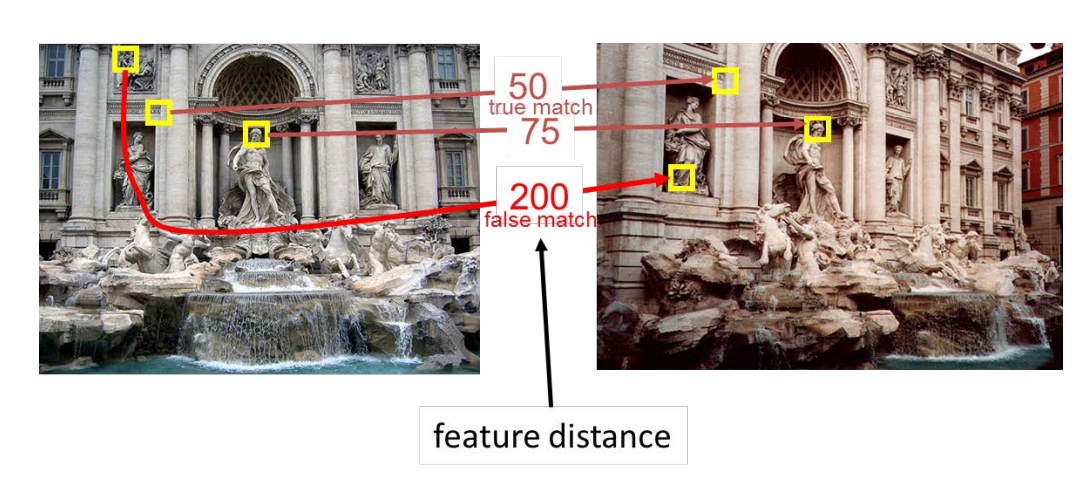
\includegraphics[width=\linewidth,natwidth=640,natheight=640]
  {fig/ref_imgs/feature_matching.png}
  \caption{Feature Mathces}
	\label{fig:feature_matchings}
\end{figure}


All being said, 
let's assume we pair consecutive images
$(\mathbf{I}_k, \mathbf{I}_{k+1})$. 
In each image, we gather feature descriptors 
$(\mathbf{D}_k^{1:n}, \mathbf{D}_{k+1}^{1:m})$ that pass through our ORB 
filter. The goal is to find the feature correspondences based on their 
rotated BRIEF descriptor values. Again, there are many efficient ways to 
perform this matching task such as FLANN 
(Fast Library for Approximate Nearest Neighbors). 
Instead, in this thesis, we choose Brute-Force matching algorithm, which
produces less outliers but it is less efficient in terms of time complexity.
The Brute-Force, as its name states, is a straightforward technique
that compares each $\mathbf{D}_{k}^{1:n}$ descriptors in $k^{th}$ image 
with $\mathbf{D}_{k+1}^{1:m}$ descriptors in $k+1^{th}$ image by calculating 
\textit{Hamming} distance:

\begin{equation}
  d_h(\mathbf{D}_{k}^i,\mathbf{D}_{k+1}^j) = \mathbf{D}_{k}^i \oplus \mathbf{D}_{k+1}^j
\end{equation}

where $\oplus$ corresponds to an 'exclusive or' logic operation. After calculating 
Hamming distances, the minimum distance are kept as best matches. On top of that, 
we perform cross-check validation by ensuring that
matches with value $(i,j)$ such that $i^{th}$ descriptor in image $k$ 
has $j^{th}$ descriptor in image $k+1$ as the best match and vice-versa.


\section{Outlier Rejection} \label{sb_sc_ransac}

In reality, not all feature matches are correct and it is critical that we 
detect wrong ones as the optimization algorithm that estimates the camera 
motion is sensitive to even small number of wrong matches. In technical terms,
we call these 
wrong matches \textit{outliers} (or \textit{false positives}). Hence, 
we need an algorithm to reject those outliers from \textit{inliers}. 
The most common way is to use RANSAC, which is an abbreviation to 
Random Sample Consensus. RANSAC is an interative algorithm which 
fits desired model with presence of outliers by selecting subset of dataset 
randomly and improving parameters of model each iteration. Note that 
RANSAC works 
well if at least half of the dataset contains inliers. 

\begin{figure}[H]
	\centering
	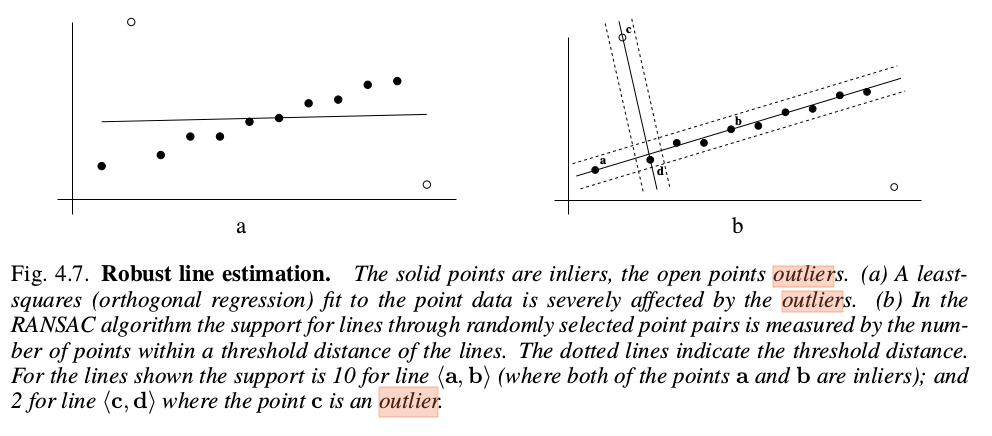
\includegraphics[width=\linewidth,natwidth=640,natheight=640]
  {fig/ref_imgs/line_ransac_outlier.png}
  \caption{Outlier Mathces}
	\label{fig:outlier_matches}
\end{figure}

In \ref{sb_sc_calibration}, we discussed how to model rotation and translation 
motion along with the intrinsic matrix. Parameteres that we aim to 
identify are elements of projection matrix in \ref{eq:proj_func_w_square_pix_skew}. 
Similarly, the model being fitted in RANSAC case is elements of a 
\textit{homography matrix}, 
which transforms a 2D image point to another 2D image point.
Remember that we have feature matches from image pairs. One of the pair is 
the transformed version of the other pair. 
We can model this relationship in the following way:

\begin{equation}
  k
  \begin{bmatrix}
    u_i' \\ v_i' \\1
  \end{bmatrix}
  =
  \mathbf{H}
  \begin{bmatrix}
    u_i \\ v_i \\1
  \end{bmatrix}
  =
  \begin{bmatrix}
    h_{00} & h_{01} & h_{02} \\
    h_{10} & h_{11} & h_{12} \\
    h_{20} & h_{21} & h_{22}
    \end{bmatrix}
  \begin{bmatrix}
      u_i \\ v_i \\1
    \end{bmatrix}
  \end{equation}\label{eq:homography_full}

The goal is to fit parameters of $\mathbf{H}$ with the selected subset of 
the matching and our assumption is majority of selected point matchings 
should be inliers. In this way, we can easily detect ourliers by testing 
whether they fit to model parameters or not. To make \ref{eq:homography_full} 
more obvious, we form linear system of equations:

\begin{equation}
\underbrace{
\begin{bmatrix}
  u_i & v_i & 1 & 0 & 0 & 0 & -u_i'u_i & -u_i'v_i -u_i'\\
  0 & 0 & 0 & u_i & v_i & 1 & -v_i'u_i & -v_i'v_i -v_i'
\end{bmatrix}}_{\mathbf{A}}
\underbrace{
\begin{bmatrix}
    h_{00} \\ h_{01} \\ h_{02} \\ h_{10} \\ h_{11} \\ h_{12} \\ h_{20} \\ h_{21} \\ h_{22}
\end{bmatrix}}_{\mathbf{h}}
= 
\begin{bmatrix}
  0\\0
\end{bmatrix}
\end{equation}

First step of RANSAC is to select a subset that contains 
minimum number of matching points to 
determine parameters of the model. In homography $\mathbf{H}$ case, we need at least 
4 point pairs $(\mathbf{p}=(u_i,v_i),\mathbf{q}=(u_i',v_i'))$ to solve 
this linear system of equation. However, due to the noise, we require more than 
4 point pairs but this makes the problem over-determined. Therefore, 
we might find an approximated solution by solving least squares problem:
With all that being said, we minimize the 
\textit{algebraic distance error}:

\begin{equation}
\argmin_h || \mathbf{Ah-0}||^2.
\end{equation}

In the second step, 
after estimating $\mathbf{h}$ paramaters, we test every matchings that are 
outside the subset which randomly selected at the first step whether 
they fit to the model with the certain $\mathbf{d}$ threshold we define:

\begin{equation}
  ||\mathbf{q} - \mathbf{H}\mathbf{p}||_2 > \mathbf{d} 
\end{equation}

In the third step, we include the points 
that passed our test procedure in the second step into our subset. In the 
forth step, we have another test. In this test, we check whether the number of 
matching points in our subset is large enough to prove that we include 
majority of the inliers. If not, we go back to first step and repeat the 
whole process again until we fulfill the fourth step. Here is the pseudo code 
that summarize the algorithm:

\begin{algorithm}[H]
  \caption{Rejecting outlier matches with RANSAC}\label{algo_ransac}

  \textbf{Input} \\
    \hspace*{\algorithmicindent}\textbf{S}: the smallest number of points\\
    \hspace*{\algorithmicindent}\textbf{N}: the number of iteration\\
    \hspace*{\algorithmicindent}\textbf{d}: the threshold used to identify a point which fits the model\\
    \hspace*{\algorithmicindent}\textbf{T}: the number of nearby points to notify that there is a good fit\\
  \textbf{Output} \\
    \hspace*{\algorithmicindent}\textbf{C}: the (consensus) set of inliers \\
  \begin{algorithmic}[1]

    \Procedure{RANSAC}{\textbf{S,N,d,T}}\\
      \While{iterations $<$ \textbf{N}}
      \State select random sample subset of \textbf{S} points
      \State estimate parameters to fit homography with \textbf{S}
      \ForEach {points outside \textbf{S}}
        \State calculate error between estimated point and measured point
        \If {error $<$ \textbf{d}}
          \State add point into \textbf{S}
        \EndIf
        \If {\textbf{S} $>$ \textbf{T}}
          \State return \textbf{C} $=$ \textbf{S}
        \EndIf
      \EndFor
      \EndWhile
    \EndProcedure
  \end{algorithmic}

\end{algorithm} \label{algo:ransac}

As it is seen in \ref{algo:ransac}, there are number of empiric parameters 
that we need to define; $\mathbf{S,N,d,T}$. To make the algorithm as 
efficient as possible, these parameters must be chosen carefully. As we 
discussed, $\mathbf{S}$ is the subset of matchings that we randomly select and 
initial value should at least 4 so that we can solve the least 
squares problem. 

For $\mathbf{N}$, it is insufficient to iterate 
through every matching points. Thus, we at least select $\mathbf{N}$ 
number of mathcing points with respect to following condition:

\begin{equation}
  \mathbf{N} = log(1-p)/log(1-(1-\epsilon)^s)
\end{equation}

where $p=0.99$ is the probability of covering all inliers, $s$ is the 
minimum number of iteration that 
probability of choosing a subset with only outliers 
and $\epsilon$ is the probability that a matching is an outlier.

For $\mathbf{d}$, it is chosen empirically if distribution of outliers is unknown. If 
it is known, i.e, Gaussian with mean $\mu$ and $\sigma$, threshold should 
be $d=5.99\sigma^2$ so that there is a 95\% probability that the point is an inlier.

For $\mathbf{T}$, we might have a case that we reach expected ratio of inliers; thus 
we don't have to iterate through $N$ number of times. We can terminate it 
ealier if the following condition is satisfied:

\begin{equation}
  \mathbf{T} = (1-\epsilon)n
\end{equation}

where $n$ is the total number of matching points.

It is crucial 
to note that we may still have outliers after 
RANSAC.
However, 
our motion estimation will be greatly improved since 
majority of the outliers are removed.
Finally, we will discuss how we can utilize the carefully selected features 
and its matches to estimate the camera motion.


\section{Pose Estimation} \label{sc_motion_estim}

TODO: SWITCH K AND C INDICES ON TRANSLATION AND ROTATION RESERVE!

Motion estimation is the core part of the VO system. After 
extracting and matching features,
we finally are ready to compute $\mathbf{T}_{k, k+1}$ transformation matrix. 
The \textit{transformation matrix} corresponds to relative camera motion information between 
two images that are recorded in different poses (see figure-\ref{fig:transformation_ij}).
Let's assume; we have 
consecutive camere poses $\mathbf{x}_k^c = [\mathbf{p}_k^c, \mathbf{q}_k^c]$ and 
$\mathbf{x}_{k+1}^c = [\mathbf{p}_{k+1}^c, \mathbf{q}_{k+1}^c]$ where 
$\mathbf{p}^c = [p_x, p_y, p_z]^T$ is the position of the camera in $\R^3$
and $\mathbf{q}^c = [q_w, q_x, q_y, q_z]^T$ is 
the orientation of the camera in quaternion form in $SO(3)$. 
Notice that, in camera model chapter 
\ref{cp_cam_models}, we used rotation matrix to represent orientations, 
which made it covenient to combine intrinsic matrix and extrinsic matrix 
(rotation and translation) into a single projection matrix 
(refer to notation \ref{eq:simplyfied_proj_func})
so that 
we optimize for paramaters of the single matrix. On the other hand, when 
estimating relative motion, we use quaternions to represent orientations, 
which is less intuitive way but 
has certain advantage over rotation matrix such as requiring less storage.
Additionally, we can represent the transformation 
$\mathbf{T}_{k,k+1}$ $(= [\mathbf{t}_{k,k+1},\mathbf{q}_{k,k+1}])$ between two camera poses 
$(\mathbf{x}_k,\mathbf{x}_{k+1})$ with the rotation $\mathbf{q}_{k,k+1}$ in $SO(3)$  
and the translation $\mathbf{t}_{k,k+1}$ in $\R^3$.

\begin{figure}[H]
	\centering
  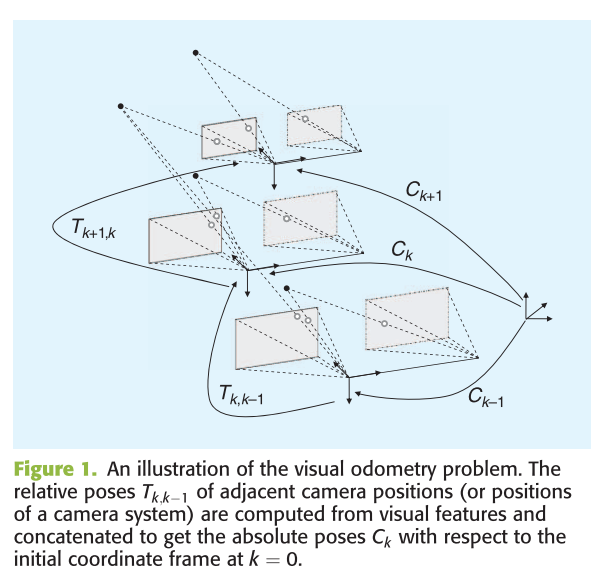
\includegraphics[width=0.7\linewidth,natwidth=640,natheight=640]
  {fig/ref_imgs/transformation_ij.png}
  \caption{GIVE EX FOR TRANSFORMATION TWO CAM POSES Transformation between Two Images}
	\label{fig:transformation_ij}
\end{figure}

That being said, one can formulate the transformation $\mathbf{T}$ 
between two camera pose. Let's first find the camera position:

\begin{equation}
  \mathbf{p}_{k+1} = 
  \mathbf{q}_{k,k+1} \otimes \mathbf{p}_k^c \otimes \mathbf{q_{k,k+1}}^* + 
  \mathbf{t}_{k,k+1}
\end{equation}

where $\mathbf{q}_{k,k+1} \otimes \mathbf{p}_k \otimes \mathbf{q_{k,k+1}}^*$ is the 
\textit{hamilton product} that is used to rotate the camera position at the $k^{th}$ pose 
and $\mathbf{t}_{k,k+1}$ is 
the simple vector addition that is used to translate the camera position. Next, 
the camera orientation can be found as follows:

\begin{equation}
  \mathbf{q}_{k+1}^c = 
  \mathbf{q}_{k,k+1} \otimes \mathbf{q}_{k}^c
\end{equation}

where $\mathbf{q}_{k,k+1}^c \otimes \mathbf{q}_{k}$ is the product of two 
quaternions that the former is the rotation and that the latter is the orientation 
of the camera at the $k^{th}$ pose.

\begin{figure}[H]
	\centering
  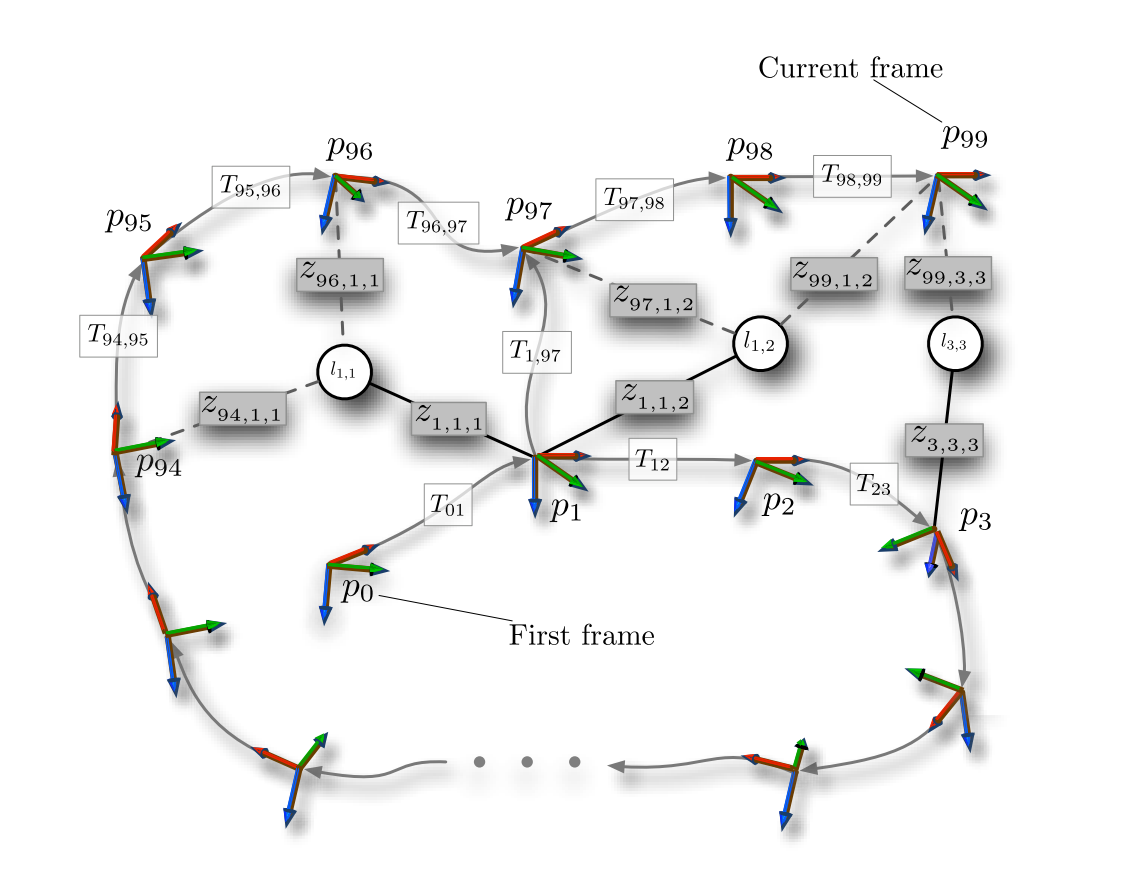
\includegraphics[width=0.7\linewidth,natwidth=640,natheight=640]
  {fig/ref_imgs/cam_trajectory.png}
  \caption{Camera Trajectory}
	\label{fig:cam_trajectory}
\end{figure}


The ultimate goal in VO is to compute transformation
$\mathbf{T}_{k,k+1}=[\mathbf{t}_{k,k+1},\mathbf{q}_{k,k+1}]$ in multiple consecutive 
images and concatenate them to build a trajectory of the camera.
As a consequence, we can track any agent on which the camera is placed rigidly. 
For example, concatenated transformation $\mathbf{T}_{0:n}$ 
can be used to calculate $n^{th}$ camera pose that is relative to the initial pose:


\begin{equation}
  \mathbf{p}_{n}^c = 
  \mathbf{q}_{n, n-1} \otimes (\dots
  (\mathbf{q}_{2,1} \otimes
  (\mathbf{q}_{1,0} \otimes \mathbf{p}_0^c \otimes \mathbf{q_{1,0}}^* + \mathbf{t}_{1,0})
  \otimes \mathbf{q}_{2,1}^* + \mathbf{t}_{2,1})
  \dots) \otimes \mathbf{q}_{n, n-1}^* +\mathbf{t}_{n, n-1} 
\end{equation}

\begin{equation}
  \mathbf{q}_{n}^c = 
  \mathbf{q}_{n,n-1} \otimes \dots \otimes \mathbf{q}_{2,1} \otimes \mathbf{q}_{1,0} \otimes \mathbf{q}_{0}^c 
\end{equation}

To find transformation, we take advantage of image features as they can 
inform us how the camera moves if we detect them across multiple frames.
All the afromentioned step such as feature extraction and feature matchings 
are performed so that we 
can compute relative motion.
Similar to projection matrix \ref{eq:proj_lsq} in camere calibration, we utilize 
the least squares method for estimating the best approximate transformation information
due to the noise. Several methods available in literature to create 
relationship between feature points that we detect across different image frames. 
%and we will discuss it in the next section.

%\subsection{Relative Pose Estimation Techniques}
%\label{sb_sc_relative_camera_pose_estimation_techniques}

So far, we discussed how we can process images so that we have adequate 
information to compute camera pose. However, we only mentioned 2D image 
features. To esimate the pose in 3D world, we require corresponding 
depth information for features. Note that there are methods that 
retrieve relative scale information using only 2D image features and its epipolar 
constraints with monocular cameras, 
but we are interested in having a metric depth information rather 
than relative scale in this thesis. Therefore, we have two common choices in terms 
of camera types: Stereo Camera or RGBD Camera. In our experiments, we experimented 
on RGBD Camera to retrieve the depth information.

At this point, one generally has two ways to compute relative camere poses.
and the reason we have different kinds of way to compute transformation arises from 
the cost function we define for the least squres problem. In the end, all we wish to 
find a good model for our optimization problem so that we settle on the 
best possible local minimum.
The design choice for cost function comes from the fact that we build 
our cost function either on $\R^2$ space (image plane) or $\R^3$ space 
(Camere Coordinate system).
Therefore, in VO literature, 
there are 2 different cost functions for modeling the least problem:
\begin{itemize}
  \item 3D-to-2D correspondences,
  \item 3D-to-3D correspondences.
\end{itemize}
The 2D term refers to 2D points that are in the image plane and that we call 
them keypoints in section-\ref{sb_sc_feature_descriptor}. 
Whereas the 3D term refers to 3D points that are in the Camera Coordinate 
System and that we call them point clouds in section-\ref{sb_sc_feature_descriptor}.

TODO: DEFINE ONE TERM FOR POINT CLOUD, FEATURE POINT OR LANDMARK. IT IS CONFUSING!

Note that this thesis does not engage with 2D-to-2D correspondences method since it is 
used in monocular camera; thus it will not be discussed here. On the other hand, 
we will discuss and compare 3D-to-2D correspondences and 3D-to-3D correspondences. 
In the motivation chapter \ref{cp_motivation}, 
I state the reasons why I chose 3D-to-3D even though it is not a common choice 
in VO literature.


\subsubsection{3D-to-2D Correspondences}

Rememeber that,
after feature matching step for the consecutive image frames, we have only
2D-to-2D keypoint correspondences information and 
the transformation which we wish to compute is in $\R^3$. Therefore, we require 
transformation involving in 3D feature points.
That being said, we can estimate transformation 3D-to-2D Correspondences in four steps:

\begin{enumerate}
  \item back-project 2D keypoints from $k+1^{th}$ frame to 3D feature points
  \item back-transform the back-projected 3D feature point from $k+1^{th}$ frame towards $k^{th}$ frame
  \item reproject the back-transformed 3D feature point onto the $k^{th}$ image plane 
  \item minimize 2D \textit{reprojection error} along with all feature matches
\end{enumerate}

\begin{figure}[H]
	\centering
  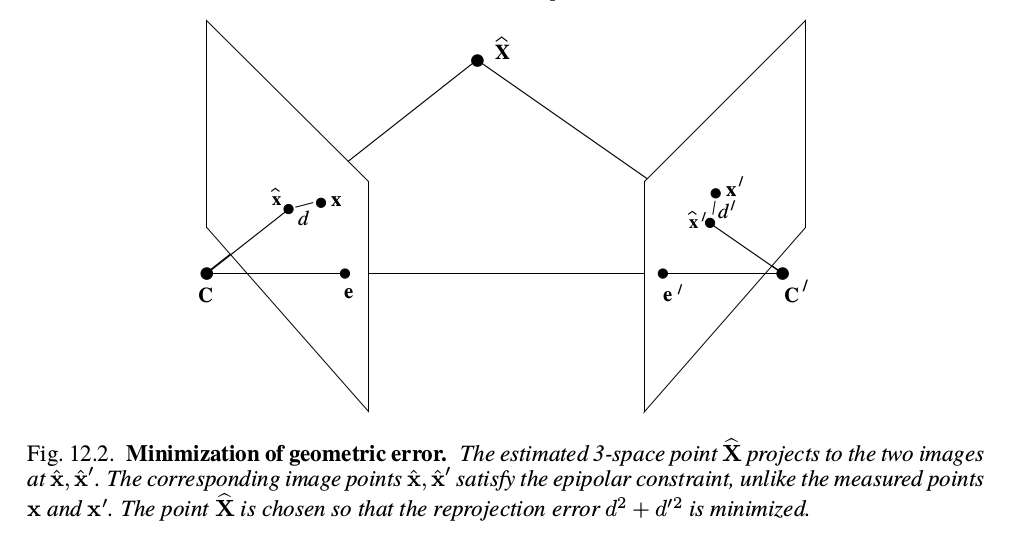
\includegraphics[width=0.7\linewidth,natwidth=640,natheight=640]
  {fig/ref_imgs/min_euclidean_error.png}
  \caption{Minimize Reprojection Error}
	\label{fig:min_geometric_error}
\end{figure}


To illustrate the 
situation more clearly, let's assume we have a 3D feature point 
$\mathbf{X}_i=[x, y, z]^T$ in Camera Coordinate System and we measure 
the projections of this exact feature point as 2D keypoint features, 
$\mathbf{x}_i^k=[u_i^k,v_i^k]^T$ and $\mathbf{x}_i^{k+1}=[u_i^{k+1}, v_i^{k+1}]^T$ 
on subsequent camera poses $k^{th}$ and $k+1^{th}$ respectively. What we also know is that 
we can back-project measured 2D keypoints to 3D feature points using projection 
matrix \ref{eq:simplyfied_proj_func_1} that we estimated in calibration process. 
Note that, since we measure 3D feature points with respect to Camera coordinate system, 
we are not interested in extrinsic matrix but only intrinsic. Now, 
let's write again projection function that converts 3D feature 
points to 2D image keypoints:
$
\mathbf{x}_i = 
  \mathbf{K}\mathbf{X}_i
  $.
One can also back-project 2D image keypoints to 3D feature points:
$
  \mathbf{K}^T\mathbf{x}_{i} = 
  \mathbf{X}_{i} 
  $.

Now, we can formulate the four steps of 3D-to-2D correspondences as follows:

\begin{enumerate}
  \item $\mathbf{X}_{i}^{k+1} = \mathbf{K}^T\mathbf{x}_{i}^{k+1}$
  \item $\mathbf{X}_i^{k'} = f(\mathbf{t}_{k,k+1}, \mathbf{q}_{k,k+1}, \mathbf{X}_i^{k+1}) = 
    \mathbf{q}_{k,k+1} \otimes \mathbf{X}_i^{k+1} \otimes \mathbf{q}_{k,k+1}^* + \mathbf{t}_{k,k+1} $
  \item $\mathbf{x}_i^{k'} = \mathbf{K}\mathbf{X}_i^{k'}$
  \item minimize $\sum_i||\mathbf{x}_i^k - \mathbf{x}_i^{k'}||^2$ where $\mathbf{x}_i^k$, $\mathbf{x}_i^{k'} \in \R^2$
\end{enumerate}

The second and third steps can be encapsulated to a function $f$ so that 
we formulate the whole optimization problem in the following form:

\begin{equation}
  \argmin_{\mathbf{t}_{k,k+1}, \mathbf{q}_{k,k+1}}
  \sum_i||\mathbf{x}_i^k - f(\mathbf{t}_{k,k+1}, \mathbf{q}_{k,k+1}, \mathbf{X}_i^{k+1})||^2
\end{equation}

This method works considerably well in practice. In VO literature \cite{}, 
it is also reported that it performs better than 3D-to-3D correspondences.

\subsubsection{3D-to-3D Correspondences}

Another way of modeling the cost function is to utilize only 3D feature point 
correspondences and one can estimate transformation with 3D-to-3D correspondences in three steps:

\begin{enumerate}
  \item back-project both 2D keypoints from $k^{th}$ and $k+1^{th}$ frames to 3D feature points
  \item back-transform the back-projected 3D feature point from $k+1^{th}$ frame
  \item minimize 3D \textit{euclidean distance} along with all feature matches
\end{enumerate}

\begin{figure}[H]
	\centering
  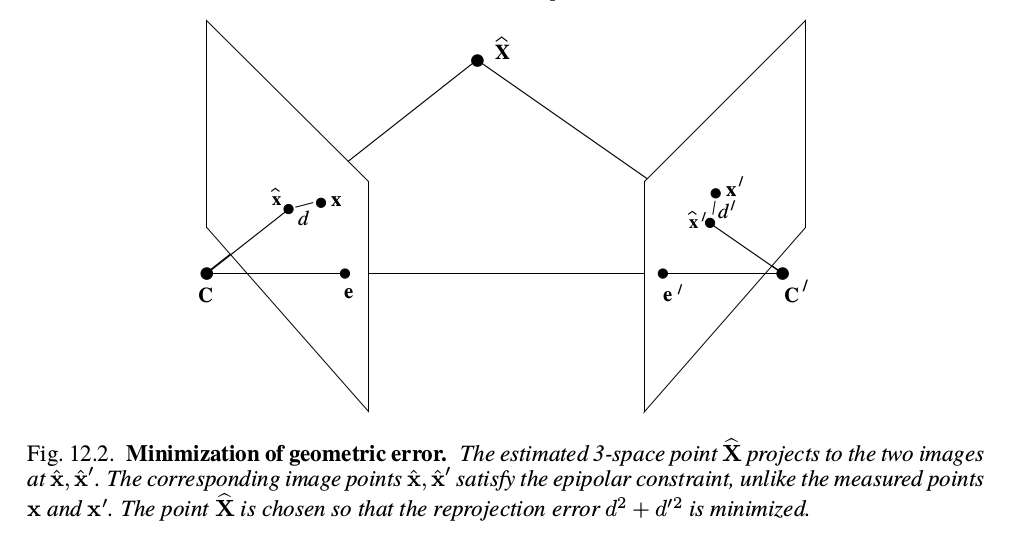
\includegraphics[width=0.7\linewidth,natwidth=640,natheight=640]
  {fig/ref_imgs/min_euclidean_error.png}
  \caption{Minimize Euclidean Error}
	\label{fig:min_euclidean_error}
\end{figure}


Similar illustrations that we previously did for 3D-to-2D correspondences applies 
for the 3D-to-3D correspondences as well but only with few changes. 
Let's again assume that we have two corresponding 2D keypoint features,
$\mathbf{x}_i^k$ and $\mathbf{x}_i^{k+1}$. However, rather minimizing error on 
2D image plane, we want to minimize them on 3D Camera coordinate system. Therefore, 
we need to back-project both keypoint features. With that in mind, 
we can formulate the three steps of 3D-to-3D correspondences as follows:

\begin{enumerate}
  \item $\mathbf{X}_{i}^{k+1} = \mathbf{K}^T\mathbf{x}_{i}^{k+1}$ and 
    $\mathbf{X}_{i}^{k} = \mathbf{K}^T\mathbf{x}_{i}^{k}$ 
  \item $\mathbf{X}_i^{k'} = f(\mathbf{t}_{k,k+1}, \mathbf{q}_{k,k+1}, \mathbf{X}_i^{k+1}) = 
    \mathbf{q}_{k,k+1} \otimes \mathbf{X}_i^{k+1} \otimes \mathbf{q}_{k,k+1}^* + \mathbf{t}_{k,k+1}$
  \item minimize $\sum_i||\mathbf{X}_i^k - \mathbf{X}_i^{k'}||^2$ where $\mathbf{X}_i^k$, $\mathbf{X}_i^{k'} \in \R^3$

\end{enumerate}

The second step can be encapsulated to a function $g$ to form the optimization 
problem:

\begin{equation}
  \argmin_{\mathbf{t}_{k,k+1}, \mathbf{q}_{k,k+1}}
  \sum_i||\mathbf{X}_i^k - f(\mathbf{t}_{k,k+1}, \mathbf{q}_{k,k+1}, \mathbf{X}_i^{k+1})||^2
\end{equation}\label{eq:3d_to_3d_rel_pose_est}

In VO literature, this method is usually discarded since 
it performs poorly comparing to 3D-to-2D correspondences.
However, we prove that it can be improved if feature covariances are properly 
estimated and included in the optimazation problem.


% ***************************CP3-MOTIVATION***************************
\chapter{Motivation} \label{cp_motivation}

The essence of a mobile robot is autonomy. 
To gain full autonomy, the robot first \textit{senses} its environment, then 
\textit{interprets} the collected data and finally \textit{acts} based on the insights 
that it gathered over time.
If we look at nature, throughout the evolution, 
certain animals gained certain abilities regarding 
spatial awareness in all sorts of ways. For instance, 
homing pigeons navigate by magnetic field, bats use sound to map their 
surroundings or bees smell with their special chemoreception to find their way 
back home. 
Even though each sense helps us with particular importance,
we humans are good at navigating ourselves by relying on our vision. 
As the incredible capability of a human eye (locating and recognizing 
objects within milliseconds even in ambiguous situations) stays a mystery, 
robotics researchers has always been keen on exploiting the computer vision field, 
especially Visual Odometry and Visual SLAM.

Visual Odometry outputs relative ego-motion information similar to IMU and 
wheel odometry. Apart from absolute sensor measurments like known a priori set of landmarks
or GPS, all of three low-level sensors are heavily used in 
localization applications as relative sensors. 
Nowadays, sensor fusion applications like SLAM and 3D reconstruction are designed 
accordingly to compensate each other's biases in order to obtain the best 
possible result. In the case of an accurate and robust sensor fusion framework, 
one selects sufficient amount absolute and relative positioning sensors. 
The ultimate goal is to fuse both relative and absolute sensor types 
along with their noise characteristics in a way that the error is minimized. 
Hence, it is critical to model each sensor's uncertainties. 
IMU and wheel odometry sensors' uncertainty are modeled by their vendors 
based on the working principles and worst-case scenario tests beforehand.
Whereas, widely used open source VO tools do not provide any uncertainty information 
about their pose estimations. Even though there are several VO papers 
\cite{Endres2014}, \cite{Konolige08}, \cite{Di2016a}, \cite{Belter2018a}
that deals with uncertainty of RGB-D sensors, they only intend to 
improve accuracy of the pose estimation, but not to provide any uncertainty 
information about their estimation. Therefore, my aim, in this thesis, is to build 
a feature-based RGB-D Visual Odometry system that outputs pose estimations 
along with their metric uncertainties.
As a result, VO system can be treated as a low-level 
relative motion sensor in a sensor fusion application.

% ***************************CP4-CoVO***************************
\chapter{An Error-Aware RGB-D Visual Odometry} \label{cp_covo}

\section{Related Works} \label{sc_error_aware_visual_odometry_related_works}

To build an error-aware VO with a RGB-D camera, 
one needs to be able to model noise characteristics of the sensor used in the 
camera. The passive stereo camera and its error propagation application 
for the uncertainty estimation are already well-studied problems 
in \cite{Leo2011} and \cite{Miura1993AnUM}.
% Uncertainty Model for Stereo Cam
% - Leo2011 - Covariance Propagation for the Uncertainty Estimation in Stereo Vision
% - Miura1993AnUM - An Uncertainty Model of Stereo Vision and its Application to Vision-Motion Planning of Robot
However, in this thesis, I am interested in implementing  
the spatial error propagation of the active stereo 
for the VO application since there is, to my knowledge, little work being done.
Beacuse our VO algorithm is a feature-based, 
quantization, introducing a systematic error in the location of detected features, 
of projected 2D points onto the image plane from 3D world using RGB camera is 
needed to be known.
This quantization error refers also as a pixel noise 
\cite{RichardHartley2003}
which is assumed to be maximum one-pixel and normally distributed in literature.
To represent the pixel uncertainty of features in 3D world, 
the conic ray model \cite{Sola2007a} is used by taking advantage of the pinhole model of 
a RGB camera. 
%However, this model can only cover uncertainties on image plane axes 
%that are perpendicular to the camera coordinate system.
% Conic Ray Model For Feature Pixel Uncertainty
% - RichardHartley2003 - Multiple View Geometry
% - Sola2007a - Towards Visual Localization, Mapping and Moving Objects Tracking by a Mobile Robot: A Geometric and Probabilistic Approach

One needs to add depth uncertainty as well. For doing so, the depth camera 
needs to be investigated. In \cite{Mallick2014b}, authors gathered existing 
studies about the depth camera's noise of Kinect. Since Kinect has two version 
that uses different technolog for measuring depth information, researchers 
compared the performance of both versions in 
\cite{Wasenmuller2017b} and \cite{Kinect2015}.
Note that we use Kinect V1 which uses the Structured-Light technique.
Another extensive paper is \cite{Khoshelham2012a}, 
outlining both a theoretical and experimental background for 
accuracy and resolution of the Kinect's depth camera based on the geometrical model.
Conversely, \cite{Choo2014} conducts a comprehensive statistical analysis 
to build a high-order polynomial mathematical model 
for the standard deviation of depth error.
% Kinect Depth Noise Model
% - Mallick2014b - Characterizations of noise in Kinect depth images: A review
% - Wasenmuller2017b - Comparison of kinect v1 and v2 depth images in terms of accuracy and precision
% - Kinect2015 - Kinect Range Sensing: Structured-Light versus Time-of-Flight Kinect
% - Khoshelham2012a - Accuracy and resolution of kinect depth data for indoor mapping applications
% - Choo2014 - Statistical Analysis-Based Error Models for the Microsoft

Even though the studies \cite{Park2012a}, \cite{Nguyen2012a} 
that deals with Kinect model the uncertainty, they don't utilize them on a 
VO system. In \cite{Park2012a}, the author contributed an important methodology on how 
to model confidence ellipsoids of 3D point clouds measured by Kinect. In this paper, 
standard deviation of the depth noise is assumed to constant; 
in fact, it increases with distance from camera quadraticly. \cite{Nguyen2012a}, however, 
addresses this issue by defining a quadratic function whose paratemeters are 
identified with optimization process. They even evaluate performance of 
their proposed model for pose estimation, which is quite relavent to our task, 
but settings of their experimentation is unclear since they focus mostly on 
3D reconstruction.
For applications such as SLAM and 3D Reconstruction, 
there are other papers \cite{Endres2014}, \cite{Konolige08}, \cite{Di2016a} that 
incorporate uncertainty models to , but 
they assume one-pixel Gaussian noise for features. Obviously, this 
increases their localization accuracy. On the other hand, it still unclear 
how one can propogate covariance of the detected features to the covariance of 
the estimated pose in the presence of outliers of matched features. 
The only exception that attempts to model the pixel 
uncertainty of features is \cite{Belter2018a}. i
They achieved it after implementing so-called 
reserve-SLAM simulation tool to identify the pixel noise caused by feature 
descriptor. The difference to 
to this thesis, they found out that feature detectors that uses edge filters 
causes error and thus they assign a confidence ellipsoid rotated along the edge.
They too perform the optimization process in the presence of outliers. 
In this thesis, I am interested in propogating the covariance of the matched features 
to the covariance of the estimated camera pose in the presence of small outliers 
after applying RANSAC.
% Similar Implementations
% - Park2012a - Spatial Uncertainty Model for Visual Features Using a Kinect™ Sensor
% - Nguyen2012a - Modeling kinect sensor noise for improved 3D reconstruction and tracking
% - Endres2014 - 3D Mapping with an RGB-D Camera
% - Konolige08 - FrameSLAM : From Bundle Adjustment to Real-Time Visual Mapping
% - Di2016a - RGB-D SLAM based on extended bundle adjustment with 2D and 3D information
% - Belter2018a - Modeling spatial uncertainty of point features in feature-based RGB-D SLAM


\section{Algorithm Description}

Before modeling uncertainties of the RGB-D camera and integrating into the VO pipeline,
we will outline the proposed error-aware VO pipeline. As many VO algorithm 
follow a standard architecture, parameter tuning process and 
algorithmic variations are performed to improve accuracy and efficiency of the system.
To build the VO, we take advantage of two commonly used open source libraries; 
i.e, OpenCV \cite{} for handling image feature manipulations and Ceres \cite{} for 
optimization.
Our proposed VO algorithm can be described in 7 steps as follows:

REVISE THESE STEPS AND REFINE THEM:
\begin{enumerate}
  \item \textbf{Extracting Feature:} 
    From grayscaled consecutive RGB frame, we use ORB that provides both 
    feature extraction with FAST corners and feature 
    descriptor with rotated BRIEF. The details of ORB can be found in 
    the previous sections \ref{sb_sc_orb}. As to parameters of ORB 
    in OpenCV, we choose number of feature as 1000, scale factor of 
    pyramid decimation ratio as 1.2, number of pyramid level as 8,  
    patch size of BRIEF as 31 and FAST corner threshold as 20 pixels. 
    These are infact default parameters except number of features.
  \item \textbf{Matching Features:} After extracting ORB features from 
    consective images, we matched them with Brute-Force algorithm that 
    uses Hamming window for the comparison. Before calling two features 
    as a match, cross check is performed to make sure both features are 
    identified as a match in their own comparison set.
    Before applying RANSAC, 
    an pre-filtering is applied by removing worst 25\% matches 
    based on distance calculated by Hamming window.
  \item \textbf{Rejecting Outliers:} With the remaining matches, we apply 
    RANSAC to reject outliers. In doing so, we choose RANSAC threshold 
    to be 10 pixels. 
  \item \textbf{Register 2D Features With Depth:} We simply combine 
    inlier 2D features with their corresponding depth information. It is 
    critical to note that Kinect has invalid depth measurement which are 
    measured as 0 disparity level for certain 
    regions of the object surface. Thus, we remove 2D features having 
    invalid depth value from match set. Plus, we remove 2D features that 
    has a depth value greater than $5m$ since it is Kinect's accurate depth 
    distance range.
  \item \textbf{Preparing Covariance Matrix of 3D Feature Points:}
    For every inlier matched features, 
    we propagate pixel uncertainties $\mathbf{Q_{uvz}}$ 
    from image plane to 
    Camera coordinate system $\mathbf{Q_{xyz}}$ with the 
    Jacobian of back-projection function $\mathbf{J_{bp}}(\mathbf{u})$
    (see notation \ref{}).
  \item \textbf{Minimizing 3D-to-3D Correspondences With Weights:}
    To able to take advantages of feature covariances of both 
    consecutive images, we expand the residuals by defining 
    both back- and forward transformation function (see notation \ref{}). 
    Then, the weighted least squares problem is solved by Levenberg-Marquardt 
    by mininizing the error between 3D-to-3D correspondences
    to calculate relative camera pose.
  \item \textbf{Calculating Covariance Matrix of the Estimated Pose:}
    After completing least squares optimization procees, we 
    calculate the covariance of the estimated relative camera 
    pose by propagating it from the feature covariances $\mathbf{Q_{xyz}}$ 
    with the Jacobian of residuals function $\mathbf{J'}(\mathbf{x^*})$ 
    at the optimal solution (see notation \ref{}).
\end{enumerate}

\section{Modeling Uncertainty of RGB-D Camera} \label{sc_modeling_uncertainty_of_rgbd}

The main reason why conventional VO applications do not provide any uncertainty 
information (namely covariance matrix) is that it is hard to model 
error characteristics of the whole VO pipeline as we perform many preprocessing, 
each of which eventually introduces different types of error. What we aim 
, in this chapter, is to define potential error source of the VO and 
to model them. To do so, we will investigate noise characteristic of 
sensors in RGB-D camera. 
Kinect, having three sensors: RGB camera, IR camera
and Ifrared (IR) laser projector as we discussed in chapter \ref{cp_cam_models}. 
In our experiments and evaluations,
we assume that these sensors are calibrated such that 
there are no registrations error when mapping RGB pixels to disparity pixels. 
Furthermore, 
we assume that measurements with these sensors are independent of each other. 
Under this asssumption, 
we split source of errors into two categories: feature related 
and depth related uncertainties.
The former is caused by feature extraction and matching algorithms. 
The latter is caused by depth camera sensor. 
In the following sections, we will discuss how we can model these 
two error sources and how to form an uncertainty model 
for the Kinect so that we estimate meaningful covariance matrices for each 
relative camera pose.

\subsection{Feature Related Uncertainty} \label{sb_sc_pixel_uncertainty}

Our VO pipeline heavily relies on the detected features 
(also called landmarks). When building such a VO system, 
it is expected that you will have a video stream that has small translation 
and rotation differences at the consecutive images. Thus, when pairing images 
to find common feature, we expect not to have high-degree rotation or large 
amount of scaling on image features so that matching algorithm would not suffer 
from high number of outliers. Under this circumstances, we identify two 
main error sources related to features; i.e., interest point location uncertainty 
and outliers in feature matching.


To understand these two types of errors, we need to remind ourselves 
how we detect and describe features section \ref{sb_sc_orb} in the first place. 
In ORB, FAST corner filter is performed by selecting pixel coordinates of an 
interest point and comparing it with its surrounding pixels. In an ideal scenario 
where we match features in consecutive image perfectly, we would assume that 
the error will be half pixel due to the quantization process of the RGB camera. 
 The ideal scenario breaks when we have outliers. What happens is that 
 we back-project features from image plane to Camera coordinate system, 
 transform them towards another image 
 and project them onto the image plane to see if how these matched interest points are 
 situated in the same image plane. If we had perfect matches, all the 
 matches would sitauted closely and the error distance between matches would
 be half pixel. However, in reality, we still have outliers even 
 after applying RANSAC. Thus, the error distance for those outliers would be 
 greater that one pixel.
 In this thesis, we call those outliers that appears after RANSAC 
 \textit{pseudo inliers}. Moreover, instead of taking pixel errors half pixel, 
 we investage the pixel error caused by pseudo inliers in section
 \ref{} and use them as pixel uncertainty.

%However, in reality, we still have outliers even after applying RANSAC. 
%What we also know that we can set a certain RANSAC threshold keep the outliers 
%within certain error boundaries. If RANSAC holds its promise, we could 
%assume the outliers will be within the RANSAC threshold. Then, outliers 
%become \textit{pseudo} inliers that has bigger interest point location uncertainty than 
%the \textit{real} inliers. At this point, we have make an approximation over 
%feature related uncertainty. In practice, RANSAC threshold would be set 
%between 1-10 pixel which already greater than uncertainty of the interest point 
%location uncertainty (which was half pixel). Therefore, we might neglect 
%interest point location uncertainty and use RANSAC threshold value for 
%calculating uncertainty of each feature.
%
%%\begin{figure}[H]
%%	\centering
%%  \includegraphics[width=0.7\linewidth,natwidth=640,natheight=640]
%%  {fig/ref_imgs/feature_related_uncertainty_one.png}
%%  \caption{Feature Related Uncertainty}
%%	\label{fig:feature_related_uncertainty_one}
%%\end{figure}
%%
%%
%%\begin{figure}[H]
%%	\centering
%%  \includegraphics[width=0.7\linewidth,natwidth=640,natheight=640]
%%  {fig/ref_imgs/feature_related_uncertainty_many.png}
%%  \caption{Feature Related Uncertainty with Many Features}
%%	\label{fig:feature_related_uncertainty_many}
%%\end{figure}
%
%
%
%
%Before we describe the conic ray model, let's consider a simple example where we 
%project 2D $\mathbf{x}$ position of a point cloud onto 1D $\mathbf{y}$ position
%as it is seen in figure-\ref{fig:conic_ray_2d_error_model}.
%
%
%\begin{figure}[H]
%	\centering
%  \includegraphics[width=0.7\linewidth,natwidth=640,natheight=640]
%  {fig/ref_imgs/conic_ray_2d_model.png}
%  \caption{Conic Ray 2D Error Model}
%	\label{fig:conic_ray_2d_error_model}
%\end{figure}
%
%Due to the errors in detected and matched features, 
%we measure the position $\mathbf{x}$ falsy. To describe how erroneous $\mathbf{x}$ 
%measurement results in false $\mathbf{y}$ positions, 
%we start formulazing it with Bayes rule:
%
%\begin{equation}
%  p(\mathbf{x}_0|\mathbf{y}_0) = \frac{p(\mathbf{x}_0) \cdot p(\mathbf{y}_0|\mathbf{x}_0)}{p(\mathbf{y}_0)}
%\end{equation}
%
%where $p(\mathbf{y}_0) = \int p(\mathbf{x}_0) \cdot p(\mathbf{y}_0|\mathbf{x}_0) d\mathbf{x}_0$
%is independent of $\mathbf{x}_0$. Assuming that we don't have any previous 
%knowledge where $\mathbf{x}$ is, the image plane is infinitely 
%large, and both $p(\mathbf{x}_0)$ and $p(\mathbf{y}_0)$ are uniform, we can transform 
%the conditional probability to pure inversion of conditionings:
%
%\begin{equation}
%  p(\mathbf{x}_0|\mathbf{y}_0) = p(\mathbf{y}_0|\mathbf{x}_0)
%\end{equation}
%
%In real-world, we measure projected points which is $\mathbf{y}$ and then 
%back-project these measures to $\mathbf{x}$. Therefore, we are interested in 
%knowing $p(\mathbf{x}_0|\mathbf{y}_0)$. For doing so, we make a further 
%assumption that the measurement noise is Gaussian. Note that, to generalize our 
%problem to all time states, we drop $k=0$ and compute for $p(\mathbf{x}|y)$. 
%First, to remind the projection functions from $\mathbf{x}=(X_{cam},Z_{cam}) \in \R^2$ to 
%$\mathbf{u}=U \in \R^1$, we write the following equation by assuming that 
%images pixel coordinates are already back-distorted and 
%intrinsic and extrinsic parameters of the RGB camera is known after calibration
%(see notation \ref{eq:proj_func_w_square_pix_skew}):
%
%\begin{equation}
%  U = f_x \frac{X_{cam}}{Z_{cam}} + c_x + \epsilon
%\end{equation}
%
%where $\epsilon$ is Gaussian additive noise. Considering what we measure 
%$y=U+\epsilon$, we can write the probability density functions
%to represent the uncertainty since we have inversion of conditioning property:
%
%\begin{equation}
%  p(\mathbf{x}|y) = \mathcal{N}(y-f_x \frac{X_{cam}}{Z_{cam}} + c_x, \sigma_u^2) \text{ or }
%  p(y|\mathbf{x}) = \mathcal{N}(f_x \frac{X_{cam}}{Z_{cam}} + c_x-y, \sigma_u^2)
%\end{equation}
%
%Notice that the back-projection axis would not pass 
%through the real $\mathbf{x}$ position because of error in features. 
%However, if we estimate the Gaussian 
%parameters sufficiently, we will have a strong idea where the measured
%point lies on XZ axis in the worst case. In statistics, one generally represent the 
%worst case scenarios with $3\sigma$ boundaries that covers  99.7\% of probability
%for one-dimensional Gaussian distribution as the following figure shows:
%
%\begin{figure}[H]
%	\centering
%  \includegraphics[width=0.7\linewidth,natwidth=640,natheight=640]
%  {fig/ref_imgs/conic_ray_2d_model_stds.png}
%  \caption{Conic Ray 2D Error Model with Different $\sigma$ Values}
%	\label{fig:conic_ray_2d_error_model_stds}
%\end{figure}
%
%So far, we only consider projections from 2D points in world onto 1D plane. 
%However, extension of this model into a model where 3D points in world are 
%projected onto 2D plane is a trivial operation: 

\begin{figure}[H]
	\centering
  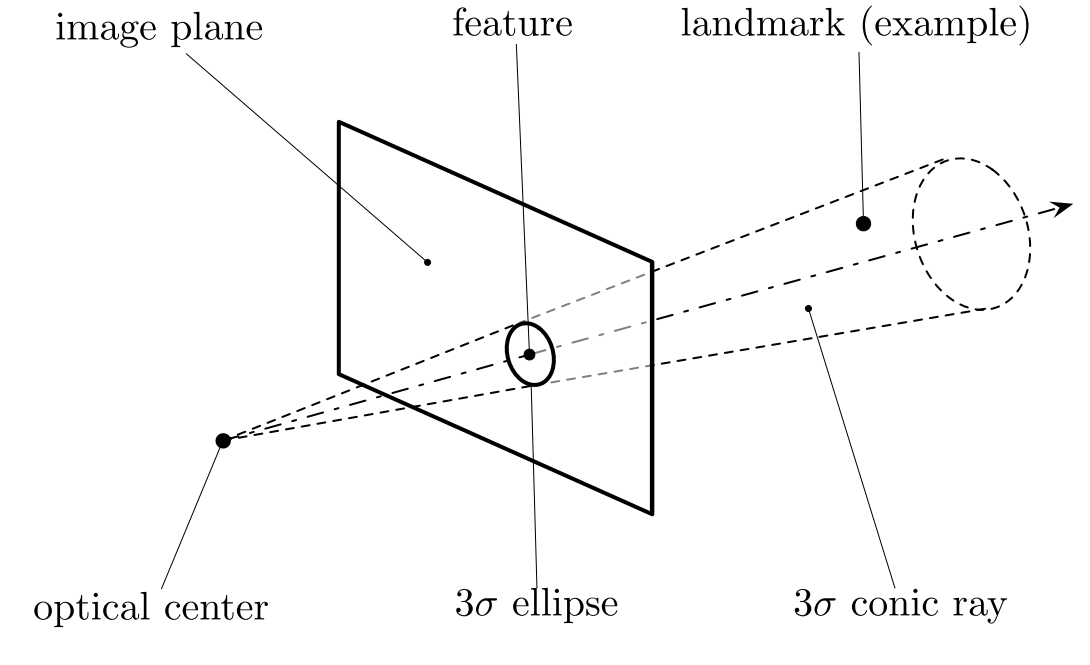
\includegraphics[width=0.7\linewidth,natwidth=640,natheight=640]
  {fig/ref_imgs/conic_ray_3d_model.png}
  \caption{Conic Ray 3D Error Model with $3\sigma$ Values}
	\label{fig:conic_ray_3d_error_model}
\end{figure}

Having all these in mind, let's model uncertainty related to features.
First of all, remember that 3D points in world are projected to 2D points on an image plane with 
Pinhole Model from section-\ref{sb_sc_pinhole}. When the aperture of a digital 
camera opens, it captures incoming light rays using its light detector sensor 
(typically CMOS image sensors) and turns them into electrical signals. That 
is an over-simplfied definition of a color camera. With the help of pinhole 
model, one can build a model for light ray coming from a 3D point. Since we 
have afromentioned errors, we can't measure the exact location of the point. 
However, it is likely that the point is within the dash line region 
(see figure \ref{fig:conic_ray_3d_error_model}) 
if the 
pinhole model is considered. In this way, we form an uncertainty region which 
we call \textit{conic ray}.
Within this conic ray, we can represent the uncertainy of a point with an 
\textit{confidence} ellipsoid if the depth uncertainty is included.
To formulate this uncertainty, we need to 
find parameters of the confidence ellipsoid
which can be represented with multi-dimensional Gaussian distributions 
in 3D space. Let's assume, it is in Camera coordinate system:

\begin{equation}
  \mathbf{g}_{xyz}(\mathbf{x}) =
  \frac{1}{\sqrt{(2\pi)^3|\mathbf{Q_{xyz}}|}} 
  \exp(-\frac{1}{2} (\mathbf{x}-\mathbf{m_x})^\intercal \mathbf{Q_{xyz}}^{-1} (\mathbf{x}-\mathbf{m_x}))
\end{equation} \label{eq:cov_ellipse}

where $\mathbf{x} = \begin{bmatrix} x \\ y \\ z\end{bmatrix}$ is the real position of the point, 
$\mathbf{m_x} = \begin{bmatrix} m_x \\ m_y \\ m_z \end{bmatrix}$ is the measured position, and
$\mathbf{Q_{xyz}} = \begin{bmatrix} \sigma_x^2 & \sigma_x\sigma_y & \sigma_x\sigma_z 
\\ \sigma_y\sigma_x & \sigma_y^2 & \sigma_y\sigma_z\\ 
\sigma_z\sigma_x & \sigma_z\sigma_y & \sigma_z^2\end{bmatrix}$ is the covariance of measurement error 
as the ellipsoid can be tilted with respect to the focal point of the camera.
With regards to measurement error in $x$ and $y$ direction, 
we only have indirect knowledge as we 
measure features on image plane in $u$ and $v$ direction.
As to measurment error in $z$ direction, we have direct knowledge 
(we assume that disparity data is already converted to depth information). 
To get errors in $x$ and $y$ directions, we need to propagate pixel uncertainties 
from image plane to Camera coordinate system. To do so, we remind ourselves 
with the back-projection function:

\begin{equation}
  \mathbf{x} = \mathbf{F_{bp}}(\mathbf{u})
\end{equation}

\begin{equation}
  \begin{bmatrix} x \\ y \\ z \end{bmatrix} =
  \begin{bmatrix} 
    \frac{z}{f_x} & 0 & -\frac{z c_x}{f_x} \\
    0 & \frac{z}{f_y} & -\frac{z c_y}{f_y} \\
    0 & 0 & z
  \end{bmatrix}
  \begin{bmatrix} u \\ v \\ 1 \end{bmatrix}
\end{equation}

\begin{figure}[H]
	\centering
  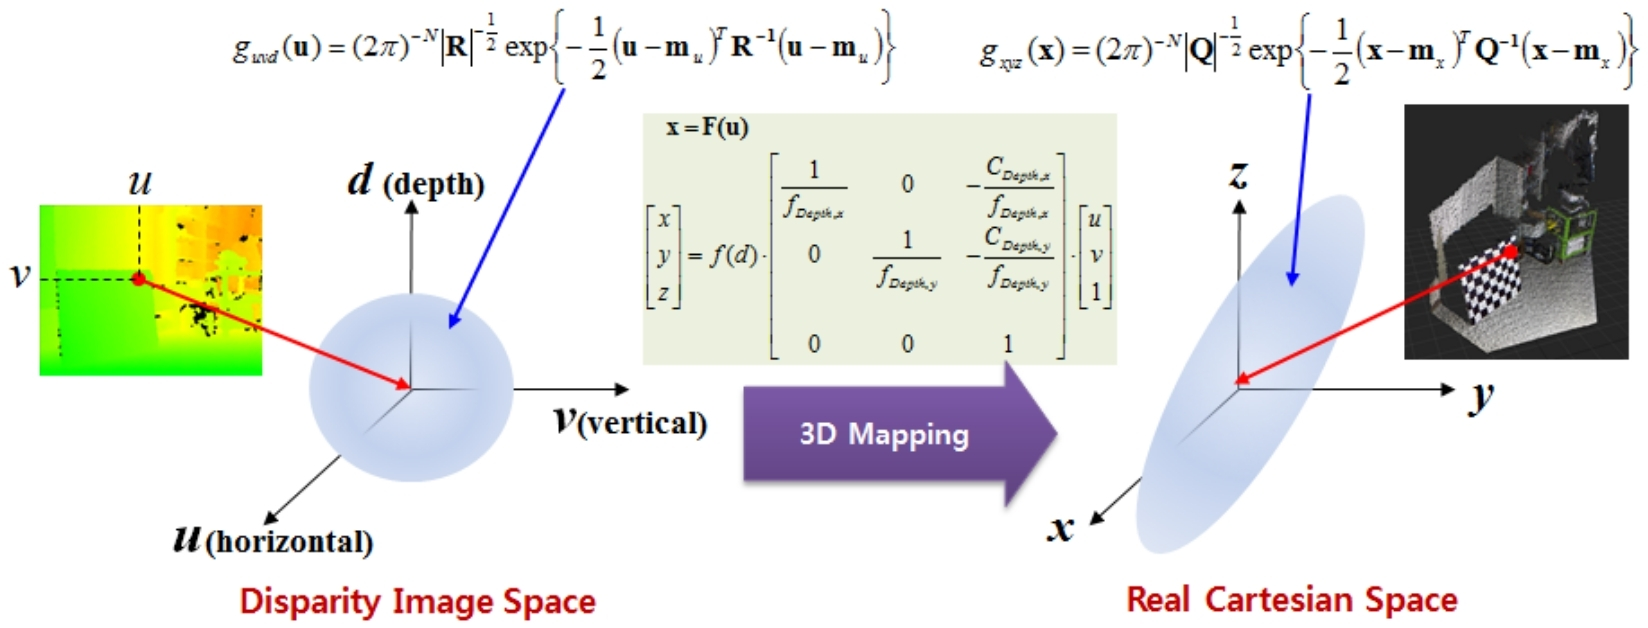
\includegraphics[width=\linewidth,natwidth=640,natheight=640]
{fig/ref_imgs/uncertainty_ellipsoid_mapping.jpg}
  \caption{Conic Ray 3D Error Model with $3\sigma$ Values}
	\label{fig:conic_ray_3d_error_model}
\end{figure}

One can represent the probability distribution of the pixel error with 
another multivarient Gaussian distribution formed by pixel uncertainties:

\begin{equation}
  \mathbf{g}_{uvz}(\mathbf{x}) =
  \frac{1}{\sqrt{(2\pi)^3|\mathbf{Q_{uvz}}|}} 
  \exp(-\frac{1}{2} (\mathbf{x}-\mathbf{m_u})^\intercal \mathbf{Q_{uvz}}^{-1} (\mathbf{x}-\mathbf{m_u}))
\end{equation} \label{eq:cov_ellipse}

where 
$\mathbf{x} = \begin{bmatrix} u \\ v \\ z\end{bmatrix}$ is the real pixel coordinate along with the real depth, 
$\mathbf{m_u} = \begin{bmatrix} m_u \\ m_v \\ m_z \end{bmatrix}$ is the noisy pixel measurements along with the noisy depth measurement, and
$\mathbf{Q_{uvz}} = \begin{bmatrix} \sigma_u^2 & 0 & 0\\ 0 & \sigma_v^2 & 0 \\ 0 & 0 & \sigma_z^2\end{bmatrix}$ is the covariance of these measument errors 
as pixel and depth measurements are considered independent.

To convert pixel error from image plane to Camera coordinate system, 
we utilize the error propagation low. In doing so, we need the partial derivative 
of the back-projection function:

\begin{equation}
  \mathbf{J_{bp}}(\mathbf{u}) = \frac{\partial \mathbf{F_{bp}}(\mathbf{u})}{\partial \mathbf{u}}  = 
  \begin{bmatrix}
    \frac{z}{f_x} & 0 & (\frac{u}{f_x} - \frac{c_x}{f_x}) \\
    0 & \frac{z}{f_y} & (\frac{v}{f_y} - \frac{c_y}{f_y}) \\
    0 & 0 & 1 
  \end{bmatrix}
\end{equation}

Then, we propogate the pixel covariances as follows:

\begin{equation}
  \mathbf{Q_{xyz}} = \mathbf{J_{bp}}(\mathbf{u})^T \mathbf{Q_{uvz}} \mathbf{J_{bp}}(\mathbf{u})
\end{equation}



%\begin{equation}
%  \mathbf{y} = \begin{bmatrix}u \\ v \end{bmatrix} \text{, } 
%  \mathbf{x} = \begin{bmatrix} f_x \frac{X_{cam}}{Z_{cam}} + c_x \\ f_y \frac{Y_{cam}}{Z_{cam}} + c_y \end{bmatrix} \text{,and }
%  \mathbf{Q} = \begin{bmatrix} \sigma_u^2 & 0 \\ 0 & \sigma_v^2 \end{bmatrix}
%\end{equation}


Apart from pixel uncertainties, 
what we haven't discussed is how we get the $\sigma_z$ depth uncertainty. 
This deserves its own explaination so we will discuss in the next section.

\subsection{Depth Related Uncertainty} \label{sb_sc_depth_uncertainty}


Modeling noise in depth measurements is more complicated than RGB camera. We 
explained how structured IR light speckles are projected onto an object 
so that IR camera can capture its disformed patterns in section \ref{sc_depth_model}. 
During this process, 
many things can go wrong. For example, (1) certain ambient background would make 
Kinect suffer from over-saturated disparity image, (2) having multiple Kinect 
in the same environment can lead to interference issue, (3) multi-path 
propagation of the light might change the expected illumination, or (4) measuring 
in dynamic scene might result in improper IR light patterns. All of these 
non-deterministic events makes it harder to model the uncertainty. However, 
we assume that operating conditions and evironment are chosen carefully 
in order to avoid these event as much as possible. What we aim to model in this 
section is mostly systematic errors in Kinect. For doing so, we rely on 
the experiments that is done by THIS GUY \cite{}. 

\subsubsection{Kinect's Systematic Depth Noise}

An experimental analysis is conducted to measure Kinect's depth noise by 
THIS GUY \cite{}. To do so, 
they calculated the difference between ground truth and Kinect measurements. 
They found out that there are two types of systematic noise occuring in Kinect's depth 
measurements: \textit{axial} noise and \textit{lateral} noise.


\begin{figure}[H]
	\centering
  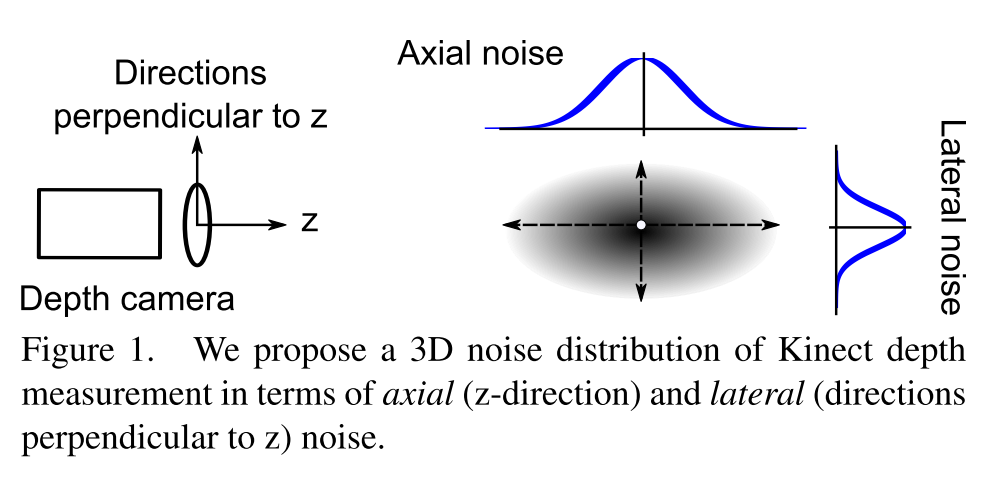
\includegraphics[width=0.7\linewidth,natwidth=640,natheight=640]
  {fig/ref_imgs/kinect_noise_model.png}
  \caption{Depth Noise}
	\label{fig:kinect_noise_model}
\end{figure}

To detect the lateral and axial noise, they built an experimental setup with a 
Kinect that projects its IR speckle patterns onto a planar surface 
(see figure \ref{fig:kinect_noise_model}). Then, they collect 
depth measurements at different distance to the planar surface 
positioning at different angles. 
For calculating the axial noise, they (1) remove the lateral noise cropping 
edges, (2) then remaining depth region is fitted a plane that has minimum 
error to the ground truth and (3) they finally calculated 
distance difference between measured depth and ground truth.
On the other hand, 
the lateral noise is simply calculated by taking pixel difference between 
fitted straight edge passing through center of distribution and 
measured (zigzag-like shape) pixels.


\begin{figure}[H]
	\centering
  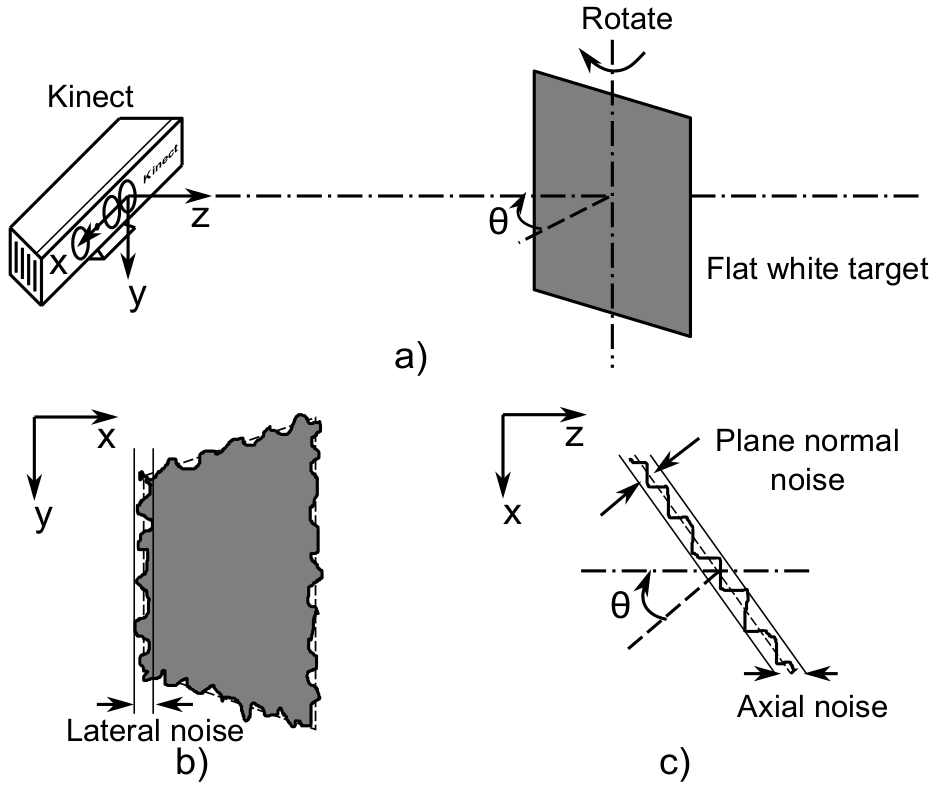
\includegraphics[width=0.7\linewidth,natwidth=640,natheight=640]
  {fig/ref_imgs/kinect_noise_experiment.png}
  \caption{Kinect Depth Noise Experiment}
	\label{fig:kinect_noise_experiment}
\end{figure}

After calculating errors between measurements and ground truth, 
they realized that the axial and lateral noise have different noise 
characteristics. The lateral noise error distribution stays constant with 
the distance as seen in figure \ref{fig:kinect_noise_hist}. Whereas, 
the axial noise distribution gets wider with the 
increased distance.


\begin{figure}[H]
	\centering
  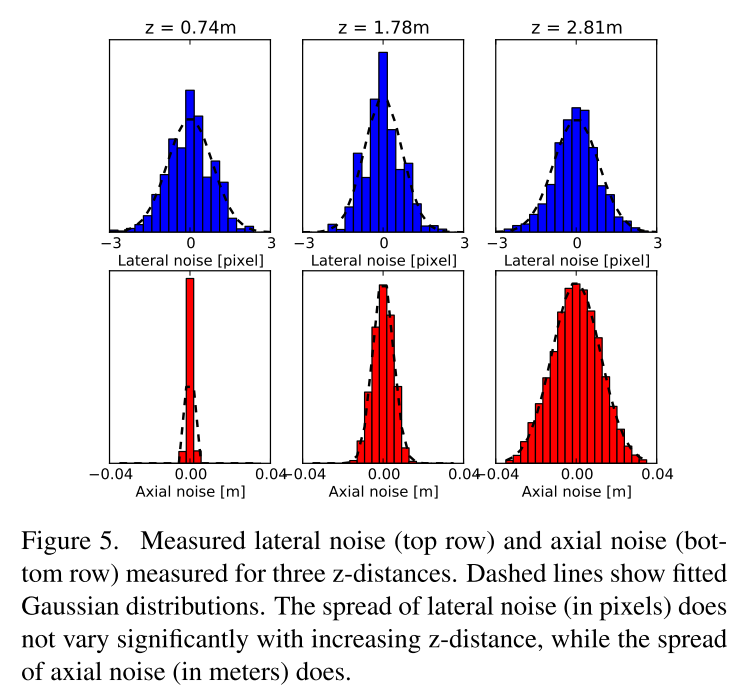
\includegraphics[width=0.7\linewidth,natwidth=640,natheight=640]
  {fig/ref_imgs/kinect_noise_hist.png}
  \caption{Kinect Depth Error Histogram at Different Distances}
	\label{fig:kinect_noise_hist}
\end{figure}

However, the axial noise has another property, which is the response to the 
different angles. Notice the following figure that shows this issue. The
standard deviation of the axial noise are increased drastically after 
60 degrees. 


\begin{figure}[H]
	\centering
  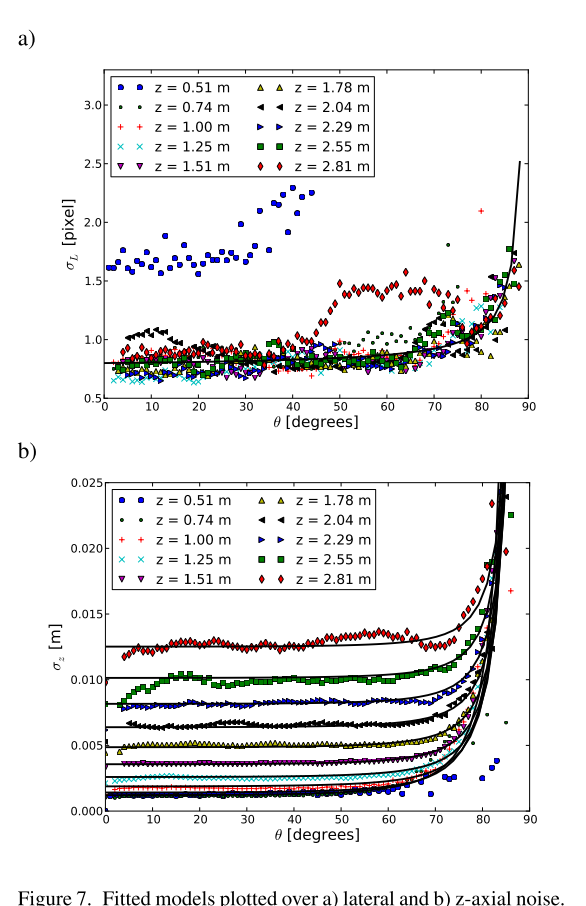
\includegraphics[width=0.7\linewidth,natwidth=640,natheight=640]
  {fig/ref_imgs/kinect_noise_fitted_model.png}
  \caption{Kinect Noise Fitted Model}
	\label{fig:kinect_noise_fitted_model}
\end{figure}

In the light of these experiments, they proposed two empirical 
models that fit corresponding measurements for the axial and lateral noise.
For axial noise, they define a 
quadratic relationship between standard deviation of the error and distance 
along z-axis. 

\begin{equation}
  \sigma_z (z,\theta) = 0.0012 + 0.0019 \cdot (z-0.4)^2 \text{, }
  \ang{10}\leq \theta \leq \ang{60}
\end{equation}

where $z$ is the measured depth metric. 
Plus, they added a hyperbolic parameter to represent the 
behavior measurement error beyond 60 degrees:

\begin{equation}
  \sigma_z (z,\theta) = 0.0012 + 0.0019 \cdot (z-0.4)^2 + 
  \frac{0.0001}{\sqrt{z}} + 
  \frac{\theta^2}{(\pi/2 - \theta)^2}
  \text{, }
  \theta \geq \ang{60}
\end{equation} \label{eq:axial_noise_w_hyperbolic}

For lateral noise, remember that its noise was almost constant with respect to 
distance along z-axis and had the similar hyperbolic effect after 60 degrees of 
angle. Hence, they defined lateral noise with the following equations:

\begin{equation}
  \sigma_L(\theta) = 0.8 + 0.035 \cdot \theta/(\pi/2-\theta) \text{ (in pixels)}
\end{equation}

This is how Kinect's depth noise is characterized experimentally by 
THIS GUY \cite{}. To validate these noise models' correctness, they implemented a 3D 
reconstruction and a camera pose tracking scenario and the noise models 
improved the overall accuracy of both application. It is important to 
note that they cooperated the iterative closest point (ICP) to estimate 
the camera poses. The ICP is one of many algorithms to solve VO problem. 
With the ICP, one utilizes all or most of the 3D point clouds instead of 
selecting distinct feature in each frame. Therefore, we need to find a way 
to integrate the depth noise model into our feature-based VO pipeline.

%\subsubsection{How To Update the Conic Ray Model with Depth Noise?}

%The missing component of our conic ray model is depth uncertainty since 
%we only defined confidence ellipses caused by feature related uncertainties so far.
%We mean the depth uncertainty that causes errors along z-axis direction. 
%This infact refers to the axial noise, which is one of Kinect's noise models 
%we discussed earlier in this section.
%Thus, we can now extend our conic ray model with the axial noise 
%(see notation \ref{eq:axial_noise_w_hyperbolic}).
%
%\begin{figure}[H]
%	\centering
%  \includegraphics[width=0.7\linewidth,natwidth=640,natheight=640]
%  {fig/ref_imgs/conic_ray_3d_model.png}
%  \caption{Conic Ray 3D Error Model with Depth Uncertainty}
%	\label{fig:conic_ray_3d_error_model}
%\end{figure}
%
%\begin{figure}[H]
%	\centering
%  \includegraphics[width=0.3\linewidth,natwidth=640,natheight=640]
%  {fig/ref_imgs/ellipsoid.png}
%  \caption{REPLACE CONFIDENCE ELLIPSE WITH ELLIPSOID}
%	\label{fig:conic_ray_3d_error_model}
%\end{figure}

Now, let's update our confidence ellipse (see \ref{eq:cov_ellipse}) formulation:

\begin{equation}
  \mathbf{Q_{uvz}} = 
  \begin{bmatrix} 
    \sigma_u^2 & 0 & 0 \\ 
    0 & \sigma_v^2 & 0 \\
    0 & 0 & (\sigma_z^{(i)}(z, \theta))^2
  \end{bmatrix}
\end{equation}

%\begin{equation}
%  \mathbf{y} = \begin{bmatrix} u_i \\ v_i \\ z_i \end{bmatrix} \text{, } 
%  \mathbf{x} = 
%  \begin{bmatrix} 
%    f_x \frac{X_{cam}}{Z_{cam}} + c_x \\ 
%    f_y \frac{Y_{cam}}{Z_{cam}} + c_y \\
%    \frac{1}{(\frac{m}{fb})d' + (Z_r^{-1} + \frac{n}{fb})}
%  \end{bmatrix} \text{,and }
%  \mathbf{Q} = 
%  \begin{bmatrix} 
%    \sigma_u^2 & 0 & 0 \\ 
%    0 & \sigma_v^2 & 0 \\
%    0 & 0 & \sigma_z(z, \theta)^2
%  \end{bmatrix}
%\end{equation}


While the axial noise can be embedded as the third dimension along the z-axis, 
the lateral noise, on the other hand, has an indirect relationship to overall 
uncertainty of a point cloud. This indirect relationship occurs when associating 
depth pixel coordinates with the color pixel coordinates, namely \textit{registration}.
Therefore, one can 
avoid this registration error by applying a smoothing filter on depth images. 
Remember that lateral noise of the Kinect was mostly around one pixel. 
Thus, a 3x3 smoothing filter can be used on extracted features or edges to compensate the error.

To summarize, we measure (1) pixel coordinates $(u^{(i)},v^{(i)})$ and 
(2) depth $z^{(i)}$ from disparity data, 
get regarding (3) intrinsic camera parameters after 
calibrating and (4) estimate pixels noise and depth axial noise by 
conducting experimental analysis before hand. If one also knows
$(X_{cam}^{(i)}, Y_{cam}^{(i)}, Z_{cam}^{(i)})$ exact coordinates of the 
3D point cloud in Camera Coordinate system
, one can simply calculate the 
probability of a measured point cloud being the real position.
On the other hand, the exact location of the point clouds are infact unknown in reality.
However, the probabilistic model, we built with the conic ray and confidence ellipsoids, 
based normally distributed noise characteristic 
can allows us to 
estimate relative camera poses by building a least squares problem.
To construct a cost function for the least squares problem, 
we need to gather (1) measured pixels, (2) measured depth, 
(3) calibrated intrinsic camera parameter and 
most importantly (4) covariance matrices of the measurements.
Having covarince matrices for the measurements not only improves the convergences 
of the optimization algorithm but also enables us to estimate a covariance matrix 
for the estimated relative pose. In the following sections, we will describe 
how to estimate relative pose of a camera and calculate a covariance 
of the estimated relative pose parameters.


\section{Pose Estimation with Uncertainties} \label{sc_rel_pose_est_w_uncertainty}

Before diving into the formulation, 
it is good idea to refresh our knowledge about how to estimate relative pose of 
a camera using 3D-to-3D correspondences in section 
\ref{sb_sc_relative_camera_pose_estimation_techniques}. 
Remember that after preprocessing extracted features, 
we would have $m$ number of measured feature matches for $k^{th}$ and $k+1^{th}$
consecutive camera frames stored as $(\mathbf{X}_{1:m}^{k}, \mathbf{X}_{1:m}^{k+1})$.
The relationship between the $k^{th}$ frame and the $k+1^{th}$ frame was 
defined with the translation $\mathbf{t}_{k,k+1}$ and 
rotation $\mathbf{q}_{k,k+1}$ information, which we also wish to calculate 
since they refer to the relative pose of the cameras as well. 
As discussed earlier, after back-projecting feaures, 
the main idea was to back-transform
the $\mathbf{X}_{1:m}^{k+1}$ features onto $\mathbf{X}_{1:m}^{k}$ feautures 
to minize the error while optimizing the translation and rotation. 
Here we define the back-transform function as follows:

\begin{equation}
  f_b(\mathbf{x}_{k,k+1}, \mathbf{X}_i^{k+1}) = 
\mathbf{q}_{k,k+1} \otimes \mathbf{X}_i^{k+1} \otimes \mathbf{q}_{k,k+1}^* + 
\mathbf{t}_{k,k+1}
\end{equation}

In traditional VO problem, the residuals function of the optimization problem 
is defined by the difference only between back-transformed point clouds from $k+1^{th}$ and 
point clouds from $k^{th}$. 

\begin{equation}
  \mathbf{t}_{k,k+1}^*, \mathbf{q}_{k,k+1}^* = 
  \argmin_{\mathbf{t}_{k,k+1}, \mathbf{q}_{k,k+1}}
  \sum_i|| \mathbf{X}_i^k - 
  f_b(\mathbf{t}_{k,k+1}, \mathbf{q}_{k,k+1}, \mathbf{X}_i^{k+1})||^2
\end{equation}

The important part of the error-aware VO that we propose in this thesis 
lies on having estimated uncertainty of the features and then to propogate it 
through uncertainty of estimated relative pose. 
If we utilized our 
conic ray model for the measured feature, we would have different 
covariance matrices for each feature.
Let's include covarince matrices into the optimization problem:

\begin{equation}
  \underbrace{\mathbf{t}_{k,k+1}^*, \mathbf{q}_{k,k+1}^*}_{\mathbf{x^*_{k,k+1}}} = 
  \argmin_{\underbrace{\mathbf{t}_{k,k+1}, \mathbf{q}_{k,k+1}}_{\mathbf{x}_{k,k+1}}}
  \sum_i|| \underbrace{\mathbf{X}_i^k - 
  f_b(\mathbf{t}_{k,k+1}, \mathbf{q}_{k,k+1}, \mathbf{X}_i^{k+1})}
  _{\mathbf{r}^{(i)}_{b}(\mathbf{x}_{k,k+1})}
||^2_{\mathbf{Q}_i^{k+1}} 
\end{equation}


However, this residuals function builds on an assumption that 
features from the $k^{th}$ frame are noise-free and 
features from the $k+1^{th}$ frame are noisy. 
Thus, we cloud only weight with $\mathbf{Q}_{1:m}^{k+1}$ as seen in the above equation.
In reality, we know that features from both frames are noisy. We can consider 
including forward-transform function such that we also take all covariance 
matrices $(\mathbf{Q}_{1:m}^{k}, \mathbf{Q}_{1:m}^{k+1})$ for all features 
into account during optimization.


\begin{figure}[H]
	\centering
  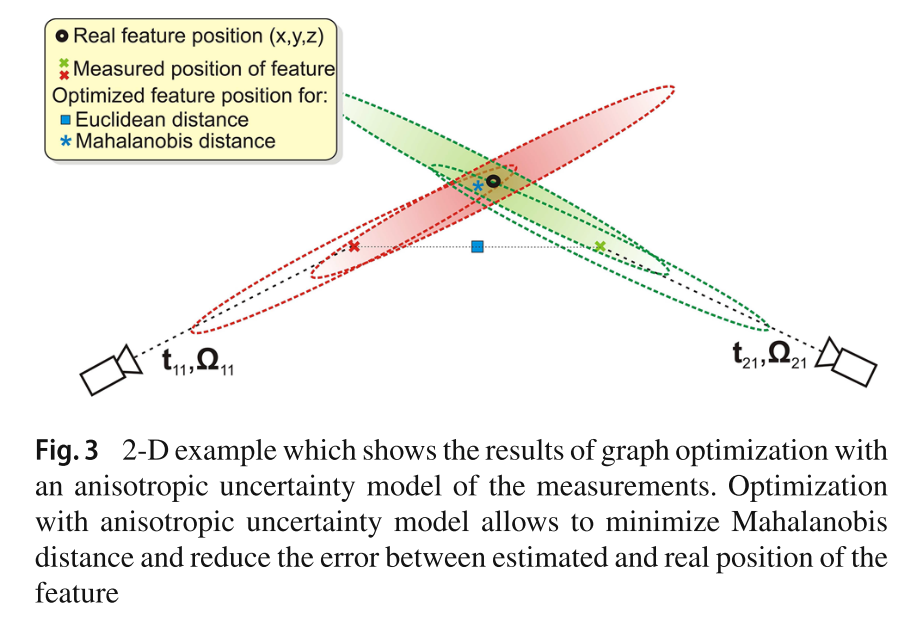
\includegraphics[width=0.7\linewidth,natwidth=640,natheight=640]
  {fig/ref_imgs/feature_related_uncertainty_one.png}
  \caption{}
	\label{fig:min_euclidean_error}
\end{figure}

With being said, we can now extend the 
residuals function of our optimization problem by adding forward-transform.
Let's define the auxilary function in the following form:

\begin{equation}
  \mathbf{r_{f}}^{(i)}(\mathbf{x}_{k,k+1}) = 
 \mathbf{X}_i^{k+1} - 
 f_f(\mathbf{x}_{k,k+1}, \mathbf{X}_i^{k})
\end{equation}

where the forward-transform function is defined as:

\begin{equation}
  f_f(\mathbf{x}_{k,k+1}, \mathbf{X}_i^{k}) = 
  \mathbf{q}_{k,k+1}^* \otimes (\mathbf{X}_i^{k} - \mathbf{t}_{k,k+1}) \otimes \mathbf{q}_{k,k+1} 
\end{equation}

Now we can reformulate our optimization problem by adding forward and back-tranformation
to each other along with corresponding covariance matrices:

\begin{equation}
  \mathbf{x^*}_{k,k+1} = 
  \argmin_{\mathbf{x}_{k,k+1}}
  \sum_i
  ||\mathbf{r_b}^{(i)}(\mathbf{x}_{k,k+1})||^2_{\mathbf{Q}_i^{k+1}}+
  ||\mathbf{r_f}^{(i)}(\mathbf{x}_{k,k+1}) ||^2_{\mathbf{Q}_i^{k}}
\end{equation}\label{eq:residuals_w_back_and_forward}

With the new auxilary function, we are able to 
minimize the error on both forward- and back-tranformation.
To take advantage of the sparsity of the matrix manipulation, we further 
modify the residuals function. Let's define, a single back-transformation operation for a single 
feature match is a $\mathbf{r_b}^{(i)}$ single residual block function. 
The same definition applies for the forward-transformation with $\mathbf{r_f}^{(i)}$.
Note that we only use $\frac{1}{2}$ in front of the residuals function for cosmetics 
reasons as it does not effect convergence of the optimization process.
%\begin{equation}
%  \begin{aligned}
%  \mathbf{x}^*_{k,k+1} = \argmin_{\mathbf{x}_{k,k+1}} &
%  %\mathbf{F(x)} & = 
%    \frac{1}{2} (||\mathbf{r_b}(\mathbf{x}_{k,k+1})||^2_{\mathbf{Q}^{k+1}} + ||\mathbf{r_f}(\mathbf{x}_{k,k+1})||^2_{\mathbf{Q}^{k}}) \\
%\end{aligned}
%\end{equation}
Then, let's reorginize the residual blocks by stacking residual blocks by columns:

\begin{equation}
\begin{aligned}
  \mathbf{x}^*_{k,k+1} := \argmin_{\mathbf{x}_{k,k+1}}
  \frac{1}{2} \begin{Vmatrix} \mathbf{r_b}^{(1)}(\mathbf{x}_{k,k+1}) \\ \mathbf{r_f}^{(1)}(\mathbf{x}_{k,k+1}) \\ 
\vdots \\ \mathbf{r_b}^{(m)}(\mathbf{x}_{k,k+1}) \\ \mathbf{r_f}^{(m)}(\mathbf{x}_{k,k+1}) 
\end{Vmatrix}^2_{\mathbf{Q}^{k},\mathbf{Q}^{k+1}} \\
\end{aligned}
\end{equation}

Above equation is the final residuals function that we are going to minize. 
The LM algorithm can be used for the optimization. I refer readers for 
further details of the LM algorithm to appendices \ref{sc_least_squares}.
However, we also need to extend regular least squares problem to 
weighted least squares problem since we multiply residual blocks with 
inverse covariance matrices. 
Let's omit $(k,k+1)$ part and generalize the problem for convenience:

\begin{equation}
  \begin{aligned}
    \mathbf{x}^* = \argmin_{\mathbf{x}} F(\mathbf{x}) = & = \argmin_{\mathbf{x}} 
  \frac{1}{2} ||\mathbf{r}(\mathbf{x})||^2_{\mathbf{Q}} \\
  & = \frac{1}{2} \mathbf{r}(\mathbf{x})^T \mathbf{Q_{uvz}}^{-1} \mathbf{r}(\mathbf{x}) \\
  & = \frac{1}{2} \mathbf{r}(\mathbf{x})^T \mathbf{\Omega}_{\mathbf{uvz}} \mathbf{r}(\mathbf{x})
\end{aligned}
\end{equation}\label{eq:residuals_objective}

where $\mathbf{\Omega_{uvz} = Q^{-1}_{uvz}}$ is the \textit{information matrix}, 
repsesent a relationship between covariance matrices and weighting process. 
That is, the smaller covariance (smaller the uncertainty in other words) for 
features, the greater weight will have in the optimization.

That being said, remember the main principle of the LM algorithm 
that is to build quadratic models 
around the initial guess and to descent to the nearest local minimum iteratively.
Thus, the new quadratic model for the weighted least squares can be written 
as follows:

\begin{equation}
  F(\mathbf{x}+\Delta \mathbf{x}) \approx q_{LM}(\Delta \mathbf{x}) = \frac{1}{2}
\mathbf{r_s}(\mathbf{x})^T\mathbf{r_s}(\mathbf{x}) + 
\mathbf{r_s}(\mathbf{x})^T\mathbf{J_s}(\mathbf{x})\Delta \mathbf{x} + 
\frac{1}{2} \Delta \mathbf{x}^T\mathbf{B_{LM,s}}(\mathbf{x})\Delta \mathbf{x}
\end{equation}

where $\mathbf{r_s}(\mathbf{x}) = \mathbf{L}^T\mathbf{r}(\mathbf{x})$ is the residuals blocks, 
$\mathbf{J_s}(\mathbf{x}) = \mathbf{L}^T \mathbf{J}(\mathbf{x})$ is the Jacobion matrix and 
$\mathbf{B_{LM,s}}(\mathbf{x}) = \mathbf{J_s}(\mathbf{x})^T \mathbf{J_s}(\mathbf{x}) + 
\lambda \mathbf{I}$ is the approximated Hessian 
matrix.
We can get the $\mathbf{L}$ matrix by the Cholesky factorization of
$\mathbf{\Omega = LL}^T$. Aftewards, we can proceed with the same calculation 
of the regular LM algorithm that we defined in the appendices.
In the end, we expect to converge to a local minimum where the translation 
and the rotation results are sufficient.

\begin{equation}
  \mathbf{x}^{n+1} = \mathbf{x}^{n} + \Delta \mathbf{x}
\end{equation}

\subsubsection{Least Squares on a Manifold}

Our ultimate goal in VO is to find the relative pose of a camera from 
$k^{th}$ frame to $k+1^{th}$ frame. 
We define a relative pose as a state vector $\mathbf{x}_{k,k+1}$. 
Through LM algorithm, we hope to 
find a optimal solution $\mathbf{x^*}_{k,k+1}$ where the residuals are minimum.
Remember that we iterately descent to the minimum by performing an 
addition operator $\Delta \mathbf{x}$ to each parameters in the state vector. 
However, one important point to note that our state vector is comprised of 
translation $\mathbf{t}_{k,k+1}$ and rotation $\mathbf{q}_{k,k+1}$. 

\begin{equation}
  \mathbf{x}^n_{k,k+1} = \begin{bmatrix} \mathbf{t}^n_{k,k+1} \\ \mathbf{q}^n_{k,k+1} \end{bmatrix} \in \R^7
  \text{ ,   } 
  \Delta \mathbf{x} = \begin{bmatrix} \Delta \mathbf{t} \\ \Delta \mathbf{q} \end{bmatrix} \in \R^6
\end{equation}

One can perform a regular $+$ addition operation with translation 
to travel on the objective function $F(\mathbf{x}_{k,k+1})$ since 
it is in Euclidean space $\R^3$ where one can add vectors to each other. 
Conversely, this does not apply for rotation 
since it is $SO(3)$ lie group in which the elements $\phi \in \R^3$ of rotation 
are in the tangent space $\mathcal{R} \in SO(3)$.
A solution to this issue would be optimizing on a manifold.
To do so, we introduce \textit{box-plus} operator
$\boxplus : \mathcal{S} x \R^n \rightarrow \mathcal{S}$ where $\mathcal{S}$ 
is an arbitrary manifold and $\R^n$ is a N-dimensional real value vector space. 
The goal is to perform small changes that are mapped to a local neighborhood in 
its own state space:

\begin{equation}
  \mathbf{x}^{n+1} = \mathbf{x}^{n} \boxplus \Delta \mathbf{x}
\end{equation}

\begin{figure}[H]
	\centering
  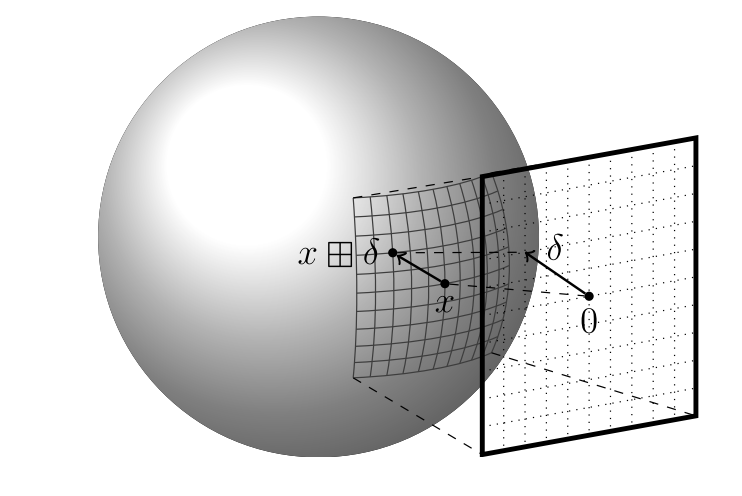
\includegraphics[width=0.5\linewidth,natwidth=640,natheight=640]
  {fig/ref_imgs/sphere_manifold.png}
  \caption{Mapping a local neighborhood in the state space}
	\label{fig:conic_ray_3d_error_model}
\end{figure}


For translating the camera with a small euclidean vector, 
one can perform regular addition since $\R^3 x \R^3 \rightarrow \R^3$:

\begin{equation}
  \mathbf{t}^n \boxplus \Delta \mathbf{t} = 
  \mathbf{t}^n + \Delta \mathbf{t} =
  \begin{bmatrix} x^{n} \\ y^{n} \\ z^{n} \end{bmatrix} + 
  \begin{bmatrix} \Delta x \\ \Delta y \\ \Delta z \end{bmatrix}
\end{equation}

NOTE:CHANGE $\R x \R$ to $\R\times \R$

For rotating, however; the box-plus operation refers to 
$SO(3) \times \R^3 \rightarrow SO(3)$ and one can rotate in its local space 
with a small unit quaternion as follows:

\begin{equation}
  \mathbf{q}^n \boxplus \Delta \mathbf{q} = 
  \mathbf{q}^n \otimes \Delta \mathbf{q} = 
  \mathbf{q}^n \otimes 
  \begin{bmatrix} \sqrt{1-||\Delta \phi||^2} \\ \Delta \phi \end{bmatrix}
\end{equation}

%\begin{equation}
%  \begin{aligned}
%  \mathbf{t}^{n+1} &= \mathbf{t}^n + \Delta \mathbf{t} \\
%  \mathbf{q}^{n+1} & = \mathbf{q}^n \otimes 
%  \begin{bmatrix} \sqrt{1-||\Delta \phi||^2} \\ \Delta \phi \end{bmatrix}
%  \end{aligned}
%\end{equation}

How does our new state vector with a manifold effect the LM algoritm? Remember 
that we form $q_{LM}(\Delta \mathbf{x})$ 
quadratic functions for each iteration around $\mathbf{x}^n$ and 
$\mathbf{J_s}$ Jacobian and $\mathbf{B_{LM,s}}$ approximated Hessian matrix 
are calculated by taking derivative of residuals function with respect to 
state vector $\mathbf{x}_{k,k+1}$. Since we modify our state vector representation 
and its corresponding updating operation, we need to modify the way we calculate 
derivatives. Here is the quadratic function with modified elements:

\begin{equation}
  F(\mathbf{x}^n \boxplus \Delta \mathbf{x}) \approx 
  q_{LM} (\Delta \mathbf{x}) = 
  \frac{1}{2}
\mathbf{r_s}(\mathbf{x}^n)^T\mathbf{r_s}(\mathbf{x}^n) + 
\mathbf{r_s}(\mathbf{x}^n)^T\mathbf{J'_s}(\mathbf{x}^n)\Delta \mathbf{x} + 
\frac{1}{2} \Delta \mathbf{x}^T\mathbf{B'_{LM,s}}(\mathbf{x}^n)\Delta \mathbf{x}
\end{equation}

One can apply chain rule to form the new Jacobian matrix:

\begin{equation}
  \begin{aligned}
  \mathbf{J'_s}(\mathbf{x}^n) = 
  \mathbf{L} \frac{\partial \mathbf{r_s}(\mathbf{x}^n)}
  {\partial \Delta \mathbf{x}} \bigg|_{\mathbf{x}^n} & = 
  \mathbf{L} \frac{\partial \mathbf{r_s}(\mathbf{x}^n)}
{\partial (\mathbf{x}^n \boxplus \Delta \mathbf{x})} \bigg|_{\mathbf{x}^n}
  \frac{\partial (\mathbf{x}^n \boxplus \Delta \mathbf{x})}
  {\partial \Delta \mathbf{x}} \bigg|_{\mathbf{x}^n,\Delta \mathbf{x}=0} \\
  & = 
  \mathbf{L}\mathbf{J}(\mathbf{x}^n) 
  \mathbf{M}(\mathbf{\mathbf{x}^n \boxplus \Delta \mathbf{x}})
  = 
  \mathbf{L}\mathbf{J'}(\mathbf{x}^n)
  = 
  \mathbf{J'_s}(\mathbf{x}^n)
\end{aligned}
\end{equation}\label{eq:new_jacobian_chain_rule}

where $\mathbf{L}$ is the matrix from the Cholesky factorization of information matrix, 
$\mathbf{J}(\mathbf{x}^n)$ is the older Jacobian matrix with the respect to 
older state vector where we assumed that all elements are in Euclidean space, 
$\mathbf{M}(\mathbf{\mathbf{x}^n \boxplus \Delta \mathbf{x}})$ is the 
matrix that we form by taking partial derivative with respect to new state vector.
Let's investigate further by breaking the new Jacobian matrix into smaller matrices 
to understand better. For weighting the optimization process, 
we assign weights with the corresponding cofindence ellipsoid of matched features 
from both consecutive frames by means of back- and forward-projection.

\begin{equation}
  \mathbf{L} 
  =
  \begin{bmatrix}
    \mathbf{L}^{(k,1)} \\
    \mathbf{L}^{(k+1,1)} \\
    \vdots \\
    \mathbf{L}^{(k,m)} \\
    \mathbf{L}^{(k+1,m)}
  \end{bmatrix}
\end{equation}

where $\mathbf{L}^{(k,i)} \text{, } \mathbf{L}^{(k+1,i)} \in \R^{3x3}$ are 
calculated from 
$\mathbf{\Omega_{uvz}}^{(k,i)} =  {\mathbf{Q_{uvz}}^{(k,i)}}^{-1}$ 
by factorization $\mathbf{\Omega = LL^T}$.
For each matched feature, 
the calculation of older Jacobian with back- and forward-projection is the following:

\begin{equation}
  \mathbf{J}(\mathbf{x}^n) = \frac{\partial 
  \mathbf{r}(\mathbf{x}^n)}{\partial \mathbf{x}^n } \bigg|_{\mathbf{x}^n}
  = 
  \begin{bmatrix}
    \horzbar & \nabla \mathbf{r}^{(1)}(\mathbf{x}^n)^T & \horzbar \\
     & \vdots & \\
     \horzbar & \nabla \mathbf{r}^{(m)}(\mathbf{x}^n)^T & \horzbar 
  \end{bmatrix}
  =
  \begin{bmatrix}
    \mathbf{J_b}^{(1)}(\mathbf{x}^n) \\
    \mathbf{J_f}^{(1)}(\mathbf{x}^n) \\
    \vdots \\
    \mathbf{J_b}^{(m)}(\mathbf{x}^n) \\
    \mathbf{J_f}^{(m)}(\mathbf{x}^n)
  \end{bmatrix}^T
\end{equation}

where $\mathbf{J_b}^{(i)}(\mathbf{x}^n) \text{, } 
\mathbf{J_f}^{(i)}(\mathbf{x}^n) \in \R^{3x7}$. Notice that in older state 
vector, we have 3 elements from translation and 4 elements from rotation of the 
quaternion. Also, here is the second partial derivative of the chain rule:

\begin{equation}
  \mathbf{M} (\mathbf{x}^n\boxplus \Delta \mathbf{x})
  =
  \begin{bmatrix}
    \mathbf{M_b}^{(1)}(\mathbf{x}^n\boxplus \Delta \mathbf{x}) \\
    \mathbf{M_f}^{(1)}(\mathbf{x}^n\boxplus \Delta \mathbf{x}) \\
    \vdots \\
    \mathbf{M_b}^{(m)}(\mathbf{x}^n\boxplus \Delta \mathbf{x}) \\
    \mathbf{M_f}^{(m)}(\mathbf{x}^n\boxplus \Delta \mathbf{x})
  \end{bmatrix}
\end{equation}

where $\mathbf{M_b}^{(i)}(\mathbf{x}^n\boxplus \Delta \mathbf{x}) \text{, } 
\mathbf{M_f}^{(i)}(\mathbf{x}^n\boxplus \Delta \mathbf{x}) \in \R^{7x6}$.
Whereas, when taking partial derivative with the respect to 
new state vector that has same 3 elements from translation and 3 elements from 
rotation as we choose the quaternion to be a unit (so-called \textit{local parameterization}).
To take the derivative with respect to new state vector, we need to consider 
Euclidean space for translation and tangent space for rotation. For translation part, 
we don't have any further effect on the new Jacobian since we stay in the same space:

\begin{equation}
  \begin{aligned}
  \mathbf{M}^{(i)}_{\mathbf{b}}(\mathbf{t}^n \boxplus \Delta \mathbf{t}) = 
    \frac{\partial (\mathbf{t}^{n} \boxplus \Delta \mathbf{t})}{\partial \Delta \mathbf{t}} 
    \bigg|_{\Delta \mathbf{t} = 0} & =
  \frac{\partial (\mathbf{t}^{n} + \Delta \mathbf{t})}{\partial \Delta \mathbf{t}}
    \bigg|_{\Delta \mathbf{t} = 0} \\
    & =
      \begin{bmatrix} 
        1 & 0 & 0 \\  
        0 & 1 & 0 \\  
        0 & 0 & 1
      \end{bmatrix} = \mathbf{I}_3
  \end{aligned}
\end{equation}

For rotation part, however; we apply chain rule one more time to take its derivative:

\begin{equation}
  \begin{aligned}
  \mathbf{M}^{(i)}_{\mathbf{b}}(\mathbf{q}^n \boxplus \Delta \mathbf{q}) = 
    \frac{\partial (\mathbf{q}^{n} \boxplus \Delta \phi)}{\partial \Delta \phi} 
    \bigg|_{\Delta \phi = 0} & =
\frac{\partial (\mathbf{q}^{n} \otimes \Delta \mathbf{q})}{\partial \Delta \mathbf{q}}
    \bigg|_{\Delta \phi = 0} 
    \frac{\partial \Delta \mathbf{q}}{\partial \Delta \phi} \\
    & =
    \frac{\partial (\mathbf{Q}^{+}(\mathbf{q}^{n}) \Delta \mathbf{q})}{\partial \Delta \mathbf{q}}
    \bigg|_{\Delta \phi = 0}
    \frac{\partial \begin{bmatrix} \sqrt{1-||\Delta \phi||^2} \\ \Delta \phi \end{bmatrix}}{\partial \Delta \phi}
    \bigg|_{\Delta \phi = 0} \\
    & =
\mathbf{Q}^{+}(\mathbf{q}^{n})
      \begin{bmatrix} 
        0 & 0 & 0 \\  
        1 & 0 & 0 \\  
        0 & 1 & 0 \\  
        0 & 0 & 1
      \end{bmatrix} \\
    & =
      \begin{bmatrix} 
        q_w^{n} & -q_x^{n} & -q_y^{n} & -q_z^{n}\\  
        q_x^{n} & q_w^{n} & -q_z^{n} & q_y^{n}\\  
        q_y^{n} & q_z^{n} & q_w^{n} & -q_x^{n}\\
        q_z^{n} & -q_y^{n} & q_x^{n} & q_w^{n}
      \end{bmatrix}
      \begin{bmatrix} 
        0 & 0 & 0 \\  
        1 & 0 & 0 \\  
        0 & 1 & 0 \\  
        0 & 0 & 1
      \end{bmatrix} \\ 
      & = 
      \begin{bmatrix} 
        -q_x^{n} & -q_y^{n} & -q_z^{n}\\  
        q_w^{n} & -q_z^{n} & q_y^{n}\\  
        q_z^{n} & q_w^{n} & -q_x^{n}\\
        -q_y^{n} & q_x^{n} & q_w^{n}
      \end{bmatrix} \in \R^{4x3}
  \end{aligned}
\end{equation}

Note that while rotating $\mathbf{q}^n$ with $\mathbf{\Delta \mathbf{q}}$, 
we utilize $\mathbf{Q}^{+}$ matrix multiplication of a quaternion rather Hamilton product 
for convenience.
If we combine both parts into a single matrix, it will be formed as follows:

\begin{equation}
\mathbf{M}_{\mathbf{b}}^{(i)}(\mathbf{x}^n \boxplus \Delta \mathbf{x}) = 
    \frac{\partial (\mathbf{x}^n \boxplus \Delta \mathbf{x})}
  {\partial \Delta \mathbf{x}} \bigg|_{\mathbf{x}^n,\Delta \mathbf{x}=0} = 
  \begin{bmatrix} 
  \mathbf{I}_3 & \mathbf{0}_{3x3} \\ 
  \mathbf{0}_{4x4} & \mathbf{M}_{\Delta \phi}   
  \end{bmatrix}
  \in \R^{7x6}
\end{equation}

As explained, we now have the new Jacobian matrix based on a manifold fashion.
Thus, we can solve the following linear system of equation as for the LM algorithm
to calculate step length:

\begin{equation}
  (\mathbf{J'_s}(\mathbf{x}_{k,k+1}^n)^T\mathbf{J'_s}(\mathbf{x}_{k,k+1}^n) 
  + \lambda^n \mathbf{I})
  \Delta \mathbf{x} =  
  -\mathbf{J'_s}(\mathbf{x}_{k,k+1}^n)\mathbf{r_s}(\mathbf{x}_{k,k+1}^n)
\end{equation}

Then, we can add corresponding small changes to the new state vector:

\begin{equation}
  \mathbf{x}^{n+1} = \mathbf{x}^{n} \boxplus \Delta \mathbf{x}
\end{equation}

After this point, we iterate through an optimal solution with the LM algorithm 
as discussed in appendices \ref{sc_least_squares}.

\section{Covariance of the Estimated Pose} \label{sc_covariance_estim}

Another important question one can ask in any kind of odometry applications is that 
what is the uncertainty, namely covariance, of the odometry measurements?
Generally, traditional VO does not provide an answer to this question 
since it does not take uncertainty of the features into account. 
However, we are now able to estimate a covariance matrix of the estimated 
translation and rotation parameter since we use the conic ray model to 
estimate feature uncertainties. 

\begin{figure}[H]
	\centering
  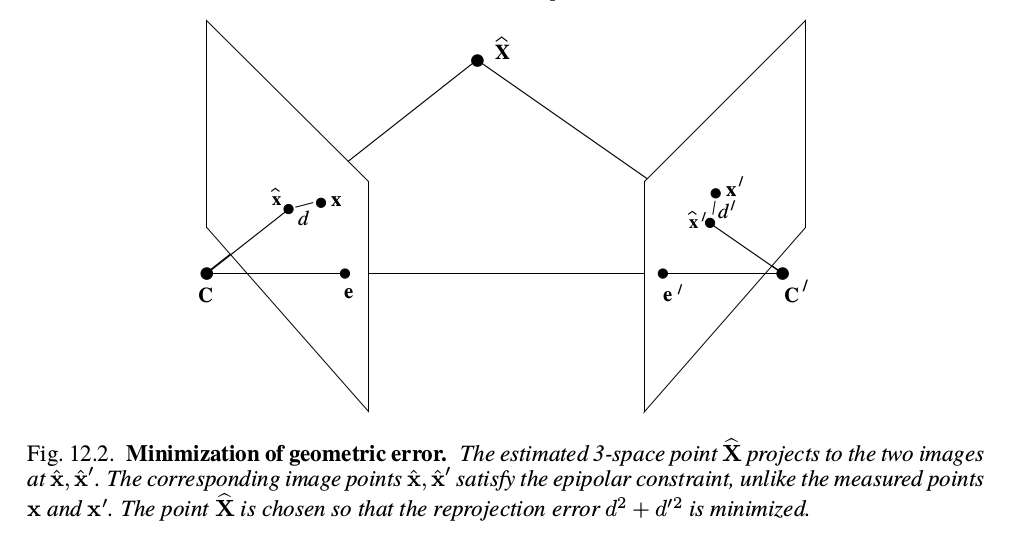
\includegraphics[width=0.7\linewidth,natwidth=640,natheight=640]
  {fig/ref_imgs/min_euclidean_error.png}
  \caption{DRAW A CONFIDENCE ELLIPSOID FOR THE ESTIMATED RELATIVE POSE}
	\label{fig:min_euclidean_error}
\end{figure}

Calculating covarinace matrix for the estimated state vector parameters is fairly 
straightforward if the optimization for the relative camera pose is performed 
as described in previous section. We can simply utilize the 
\textit{error propagation law} 
(I refer readers for to appendices \ref{sc_error_prop_law} for further details 
of it). 
For doing so, we require the Jacobian matrix 
at the optimal solution and corresponding covariance  
matrices for each matched feature. Then, we can propagate them to get the 
covariance for the estimated parameters by applying the following equation:

\begin{equation}
\mathbf{Q_{\mathbf{t},\mathbf{q}}}^{k,k+1} = (\frac{1}{2})^2 \cdot \mathbf{J'}(\mathbf{x^*}_{k,k+1})^T \mathbf{Q_{xyz}}^k \mathbf{J'}(\mathbf{x^*}_{k,k+1})
\end{equation}\label{eq:error_prop_cam_pose}

where 
$\mathbf{J'}(\mathbf{x^*}_{k,k+1}) \in \R^{6mx6}$ 
is the Jacobian of extended residuals function with back-,forward-transformation and 
manifold in \ref{eq:new_jacobian_chain_rule},

\begin{equation}
\begin{aligned}
  & \mathbf{Q_{xyz}}^{k,k+1} = \begin{bmatrix} 
  \mathbf{Q_{xyz}}^{(k,1)} & \dots & & &\mathbf{0} \\
  \mathbf{0} & \mathbf{Q_{xyz}}^{(k+1,1)} & &\dots & \vdots  \\
   \vdots & & \vdots &  &\\
   &  & & \mathbf{Q_{xyz}}^{(k,m)} & \mathbf{0} \\
   \mathbf{0} &  & & & \mathbf{Q_{xyz}}^{(k+1,m)}
  \end{bmatrix} \in \R^{6mx6m}
\end{aligned}
\end{equation}

is the covariance matrix that comprised of all covarince matrices for all 
matched features from $k^{th}$ and $k+1^{th}$ consecutive frames,

\begin{equation}
\begin{aligned}
  & \mathbf{Q_{xyz}}^{(k,i)} = 
  \mathbf{J_{bp}}^T(\mathbf{u})
  \begin{bmatrix} 
    \sigma_u^2 & 0 & 0 \\ 
    0 & \sigma_v^2 & 0 \\
    0 & 0 & (\sigma_z^{(i)}(z, \theta))^2
  \end{bmatrix} \mathbf{J_{bp}}(\mathbf{u}) \in \R^{3x3}
\end{aligned}
\end{equation}

is the covarince matrix for the $i^{th}$ matched feature from $k^{th}$ frame,

\begin{equation}
\begin{aligned}
  & \mathbf{Q_{\mathbf{t},\mathbf{q}}}^{k,k+1}  = \begin{bmatrix} 
  \sigma_{t_x}^2 & 0 & 0 & 0 & 0 & 0 \\ 
  0 & \sigma_{t_y}^2 & 0 & 0 & 0 & 0 \\
  0 & 0 & \sigma_{t_z}^2 & 0 & 0 & 0 \\
  0 & 0 & 0 & \sigma_{q_x}^2 & 0 & 0 \\
  0 & 0 & 0 & 0 & \sigma_{q_y}^2 & 0 \\
  0 & 0 & 0 & 0 & 0 & \sigma_{q_z}^2
  \end{bmatrix} \in \R^{6x6}
\end{aligned}
\end{equation}

is the resulting covariance matrix for the estimated state vector paramaters 
(in other other words, it is the uncertainty of the estiamted pose of the camera)
for $k^{th}$ and $k+1^{th}$ consecutive frames, 
$m$ is the the number of measured feature matches.
Notice $(\frac{1}{2})^2$ in front of \ref{eq:error_prop_cam_pose}. This multiplication 
corresponds to the back- and forward-transformation of residuals function. 
To be more clear, remember that 
we represented a relative camera motion with both back and forward 
transformation in order to take errors on both $k^{th}$ and $k+1^{th}$ 
consecutive images into account. This resulted in having two residuals 
$\mathbf{r_b}^{(i)}$ and $\mathbf{r_f}^{(i)}$ 
for one feature match (see notation \ref{eq:residuals_w_back_and_forward}). 
Therefore, we divide by 2. The reason we square it is beacuse of the covariance.

\chapter{Evaluation} \label{cp_evaluation}
% ***************************CP5-EVALUATION***************************

Computer vision applicatons like VO require many approximations and linearization 
techniques in order to cope with its dynamic nature for the sake of efficiency.
In practice, many corner cases might occur, no matter how 
good such estimation algorithms are modeled. It is therefore critical 
to verify such systems. Considering that 
the proposed error-aware VO algorithm outputs two information: 
relative pose estimation and its covariance estimation, 
this chapter will be mainly built around two following questions 
that I am going ask:

\begin{enumerate}
  \item What is the \textit{accuracy} of relative pose estimations?
  \item How \textit{consistent} do the algorithm estimate 
    covariance of its pose?
\end{enumerate}

In order to tackle with these questions, simulation environment will 
used to validate the model at first. Then, RGB-D datasets will be used 
to test the algorithm in real-worl environment.

\section{Error Metrics}

There are already 
well-established error evaluation methods in literature so I 
am going to follow them in order to better 
understand characteristics of the proposed algorithm.
If we want to apply these methods on our algorithm, we need to have 
the ground truth pose sequences $\mathbf{x}_{1:n} \in SE(3)$ for 
comparing with the estimated pose sequences $\mathbf{x^*}_{1:n} \in SE(3)$. 
In our calculations, we asumme that both pose sequences are
time-synchronized, equally sampled and have the same length $n$.
However, it is important to note that none of these assumptions are hold 
so we need to be aware of the error caused by these issues. 

\subsubsection{Relative Pose Error}

For evaluating the accuracy of a VO algorithm, it is better 
calculate the relative pose error rather than comparing with the 
absolute (whole) estimated trajectory. This is also refered as Relative 
Pose Error (RPE). 
On the other hand, some VO estimate a relative pose by frame-to-frame and 
some VO by keyframes. 
To able to compare all kinds of VO with each other, a fixed time interval 
$\Delta$ is chosen to calculate the local accuracy of the pose estimation. 
In this way, we take local drifts into account to compare both types of VO algorithms.
Thus, we defined RPE at time instance $i$ as follows:

\begin{equation}
  \mathbf{E}_i := 
  (\mathbf{x}_i^{-1} \mathbf{x}_{i+\Delta})^{-1} 
  (\mathbf{x^*}_i^{-1}\mathbf{x^*}_{i+\Delta})
\end{equation}

One can take a mean of all $E_{1:n}$ RPE, but this hides 
the effect of outliers when $n$ is large.
Instead , we calculate Root Mean Error Squared (RMSE) which compresses the 
error with much more information since it takes mean deviation of the error.
%\subsubsection{Root Mean Squared Error of RPE}
RMSE will show how the mean deviation of the error. For doing so,
$m = n - \Delta$ number of RPE are required to be calculated 
among $n$ pose sequences,:

\begin{equation}
  RMSE(\mathbf{E}_{1:n},\Delta) := \sqrt{\frac{1}{m} \sum_{i=1}^{m}||\mathbf{E}_i||^2}
\end{equation}

Then, we take a mean of all RMSE over whole trajectory:

\begin{equation}
  RMSE(\mathbf{E}_{1:n}) :=  \frac{1}{n} \sum_{\Delta=1}^{n}RMSE(\mathbf{E}_{1:n},\Delta)
\end{equation}

It is important to note that we take $\Delta=1$ when we want to know 
a drift per frame. This is useful when comparing simulation results with 
real world experiments for the same algorithm. 
Conversely, we take $\Delta=30$ when comparing 
the proposed algorithm other VO. This corresponds to a drift per approximately 
1 second.

\subsubsection{Normalized Estimation Error Squared}

The main focus of this thesis is to provide metric uncertainty of the relative 
pose. We do this by propogating the uncertainty of the 3D features points 
through the error model. In this case, it is critical to assess 
consistency of estimated convariance values to gain trust for  
filter-based or graph-based sensor fusion applications. 
One of the good metrics to evaluate consistency is 
to calculate Normalized Estimation Error Squared (NEES). This method measures 
the credibility of the provided covariance and it helps us to decide whether 
the predicted uncertainty values are optimisic or pessimistic.
One can calculate NEES if $\mathbf{x}_i$ real pose, $\hat{\mathbf{x}_i}$ predicted 
pose and $\Omega_i = \mathbf{Q}_i^{-1}$ information matrix are known at time 
instance $i$:

\begin{equation}
  \epsilon_i = (\mathbf{x}_i - \mathbf{x^*}_i)^T \mathbf{\Omega}_i (\mathbf{x}_i - \mathbf{x^*}_i) 
  = ||\mathbf{e}_i||^2_{\Omega_i}
\end{equation}

%\subsubsection{Average Normalized Estimation Error Squared (ANEES)}

We also take an average of NEES (ANEES) over whole trajectory:

\begin{equation}
  d \hat{\epsilon} =  \frac{1}{n} \sum_{i=1}^{n} \epsilon_i = 
  \frac{1}{n} \sum_{i=1}^{n} ||\mathbf{e}_i||^2_{\Omega_i}
\end{equation}

NOTE: find a synonym for it is important to note phrase!

If the system is linear, has degree of freedom $d=1$ and gaussian noise, 
then the expected value 
$\hat{\epsilon}$ is 1. However, in practice, this does not hold. Therefore, 
another metric when deciding on whether the estimator is consistent or not
is to look at the distribution of NEES over trajectory, which is 
distributed as a chi-square $\chi_d^2$ with $d$ degrees of freedom. 
For an estimator with 3 degree of freedom, acceptance region is
$\hat{\epsilon} \in [2.5,3.5]$ 
when significance level $\alpha$ of $\chi_d^2$ 
is chosen 2.5\% and 50 Monte Carlo runs according to [\cite{Shalom2001}, pp.234-235].
It is important to note that 
we did not implement Manto Carlo simulation for our simulation environment. 
We only treat each estimation as an independent event by adding 
random gaussian noise to the measurements. Thus, when evaluating 
consistency of the estimator in simulation, we aim to get 
$\hat{\epsilon_t}=3$ for translation and $\hat{\epsilon_q}=3$
since both have 3 degree of freedom. On the other hand, when testing 
the estimator with real-world data, we only take upper boundary of 
acceptance region $\hat{\epsilon_t} \in [0, 3.5]$ and 
$\hat{\epsilon_q} \in [0, 3.5]$ since it is 
acceptable to have a conservative estimator rather than overconfident one.


\section{Simulation Environment}

Before testing the proposed algorithm, we will validate the relative 
pose estimation and its covariance with the simulated data. To do so, 
we create a 3D simulation environment that consists of a camera pose, 
3D feature points and their confidence ellipsoids. Our test scenario 
will be comprised of the following steps:

\begin{itemize}
  \item 500 3D feature points are created within camera's observable space.
  \item By utilizing the pinhole model, 
    all 3D feature points are projected onto the camera whose initial pose $p_0$ is known.
  \item Projected feature points are stored in the form of 
    $(u_{1:500}^{0}, v_{1:500}^{0},z_{1:500}^{0})$ sensor measurements as you would usually get it from 
      a regular RGB-D camera. 
    \item The camera is transformed (translated and rotated) with a known distance 
      and rotation $\mathbf{x}_{0,1} = [0.6, 0.6, 0.05, -0.183, -0.183, 0, 0.966]$ 
      to its next pose $p_1$. 
    \item The same 3D feature points are projected with respect to the new pose $p_1$ 
      and stored as $(u_{1:500}^{1}, v_{1:500}^{1},z_{1:500}^{1})$.
    \item In order to introduce uncertainty into the system, the gaussian 
      noises are added on both sensor measurements independently
      $(\hat{u}_{i}=u_{i}+\phi_u, 
      \hat{v}_{i}=u_{i}+\phi_v,
    \hat{z}_{i}=z_i+\phi_z)$ where $\phi\sim\mathcal{N}(\mu,\sigma)$:
      \begin{itemize}
          \item The pixel noises are
            assigned to $(\mu_u=0,\sigma_u=8)$ and $(\mu_v=0,\sigma_v=8)$. 
          \item Whereas, 
            mean of depth noise is $\mu_z=0$ and standard deviation is chosen 
            with respect to feature points' distance to the camera.
            $\sigma_z^i (z,\theta)$. 
            The lateral noise and the surface angle $\theta$ is assumed to be 0.
            The depth's noise model is discussed in \ref{sb_sc_depth_uncertainty}.
        \end{itemize}
    \item For every measurements, convariance matrices 
      $(\mathbf{Q}_{xyz}^{0,1:500}, \mathbf{Q}_{xyz}^{1,1:500})$ are formed with 
      the same standard deviations of the added noises, where  
      $\mathbf{Q_{xyz}}^{(i)} = \mathbf{J_{bp}}(\mathbf{u})^T
  \begin{bmatrix} 
    \sigma_u^2(=8^2) & 0 & 0 \\ 
    0 & \sigma_v^2(=8^2) & 0 \\
    0 & 0 & (\sigma_z^{(i)}(z, \theta))^2
  \end{bmatrix} \mathbf{J_{bp}}(\mathbf{u})$.

    \item Perfectly matched noisy 3D feature point pairs along with their covariances 
      are given to the optimizer that is discussed in \ref{sc_rel_pose_est_w_uncertainty} 
      to estimate $\mathbf{x^*}_{0,1}$ and $\mathbf{Q}_{\mathbf{t,q}}^{0,1}$.
    \item This whole process is repeated 1000 times.
\end{itemize}

In the following simulation figures, we implement discussed scenario into 
a 3D space. In this environment, we have  
noisy 3D feature points, confidence ellipsoids whose center is around the 
noisy feature points and real position of the 3D feature points that are somewhere 
inside the ellipsoids.

% Distribution of Point Clouds in 3D at p0
\begin{figure}[H]
  \centering
  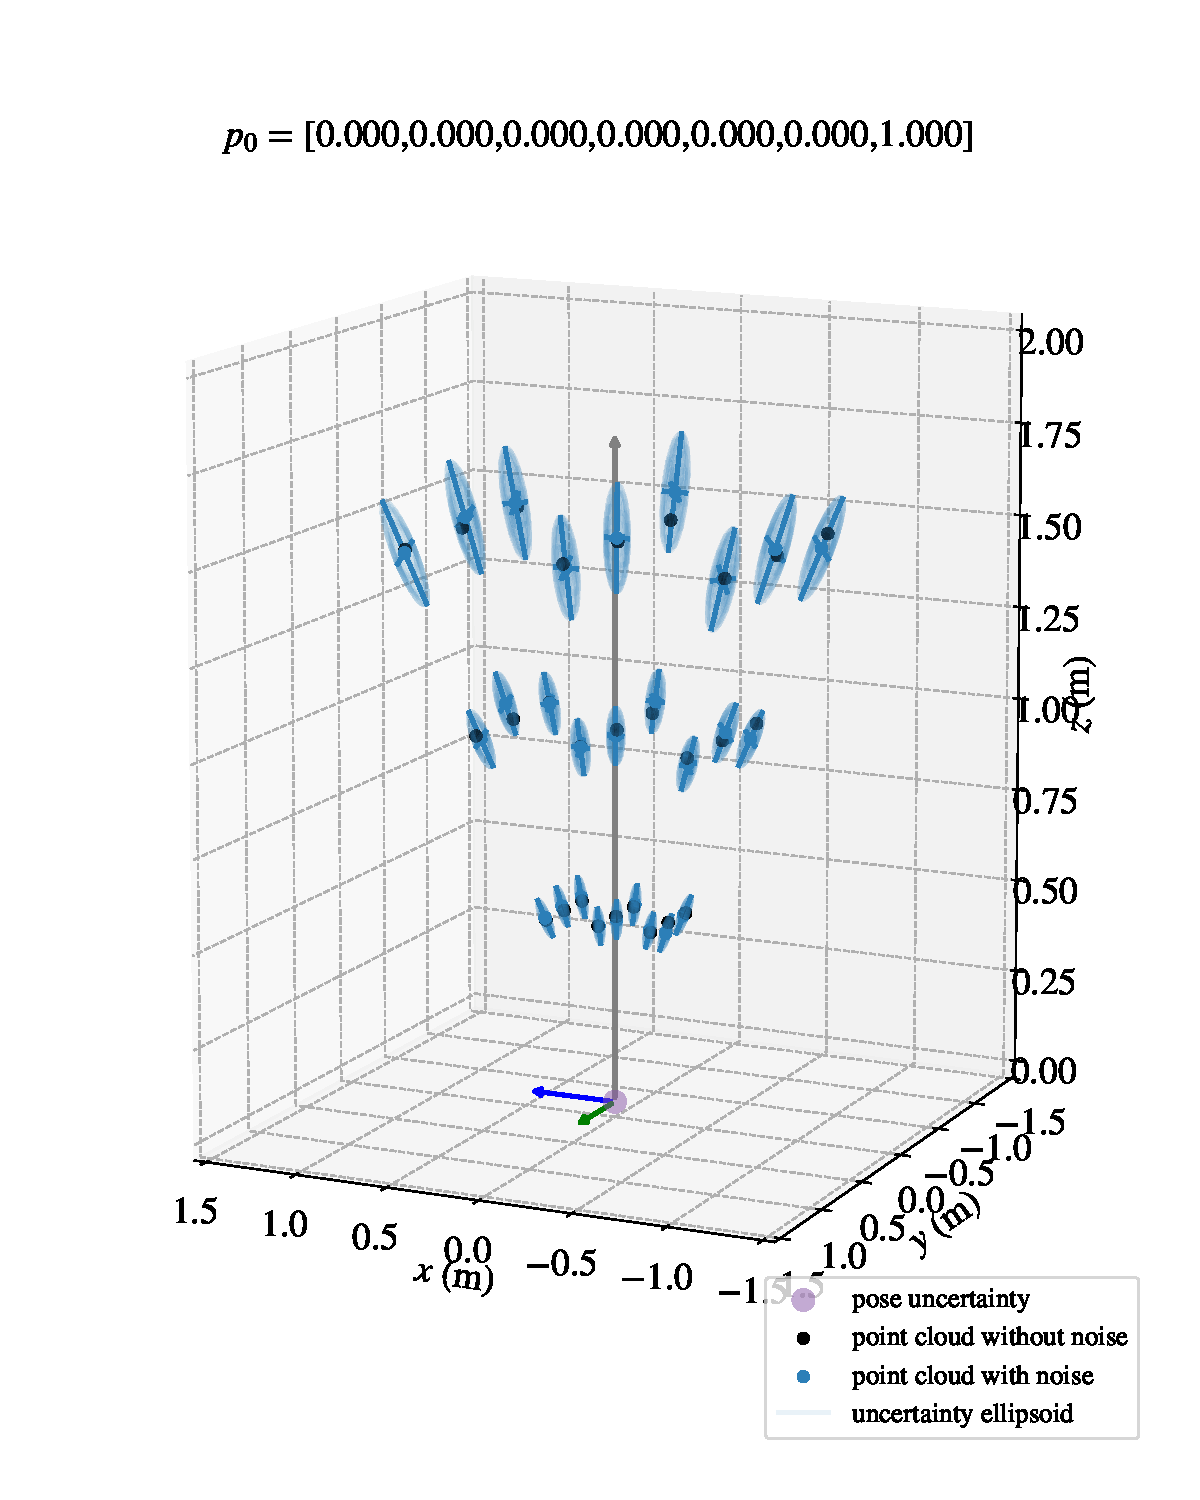
\includegraphics[width=\linewidth,natwidth=640,natheight=640]
  {fig/eva_graphs/sim_at_p0.pdf}
  \caption{asda}
	\label{fig:sim_at_p0}
\end{figure}

The figure \ref{fig:sim_at_p0} depicts the environment at its initial pose $p_0$. 
Note that we only draw small subset of 3D feature points and scaled the 
confidence ellipses by 10 to gain visibility. Notice how 
size and orientation of the confidence ellipsoids are situated according to 
the conic ray model.


% Distribution of Point Clouds in 3D at p1
\begin{figure}[H]
  \centering
  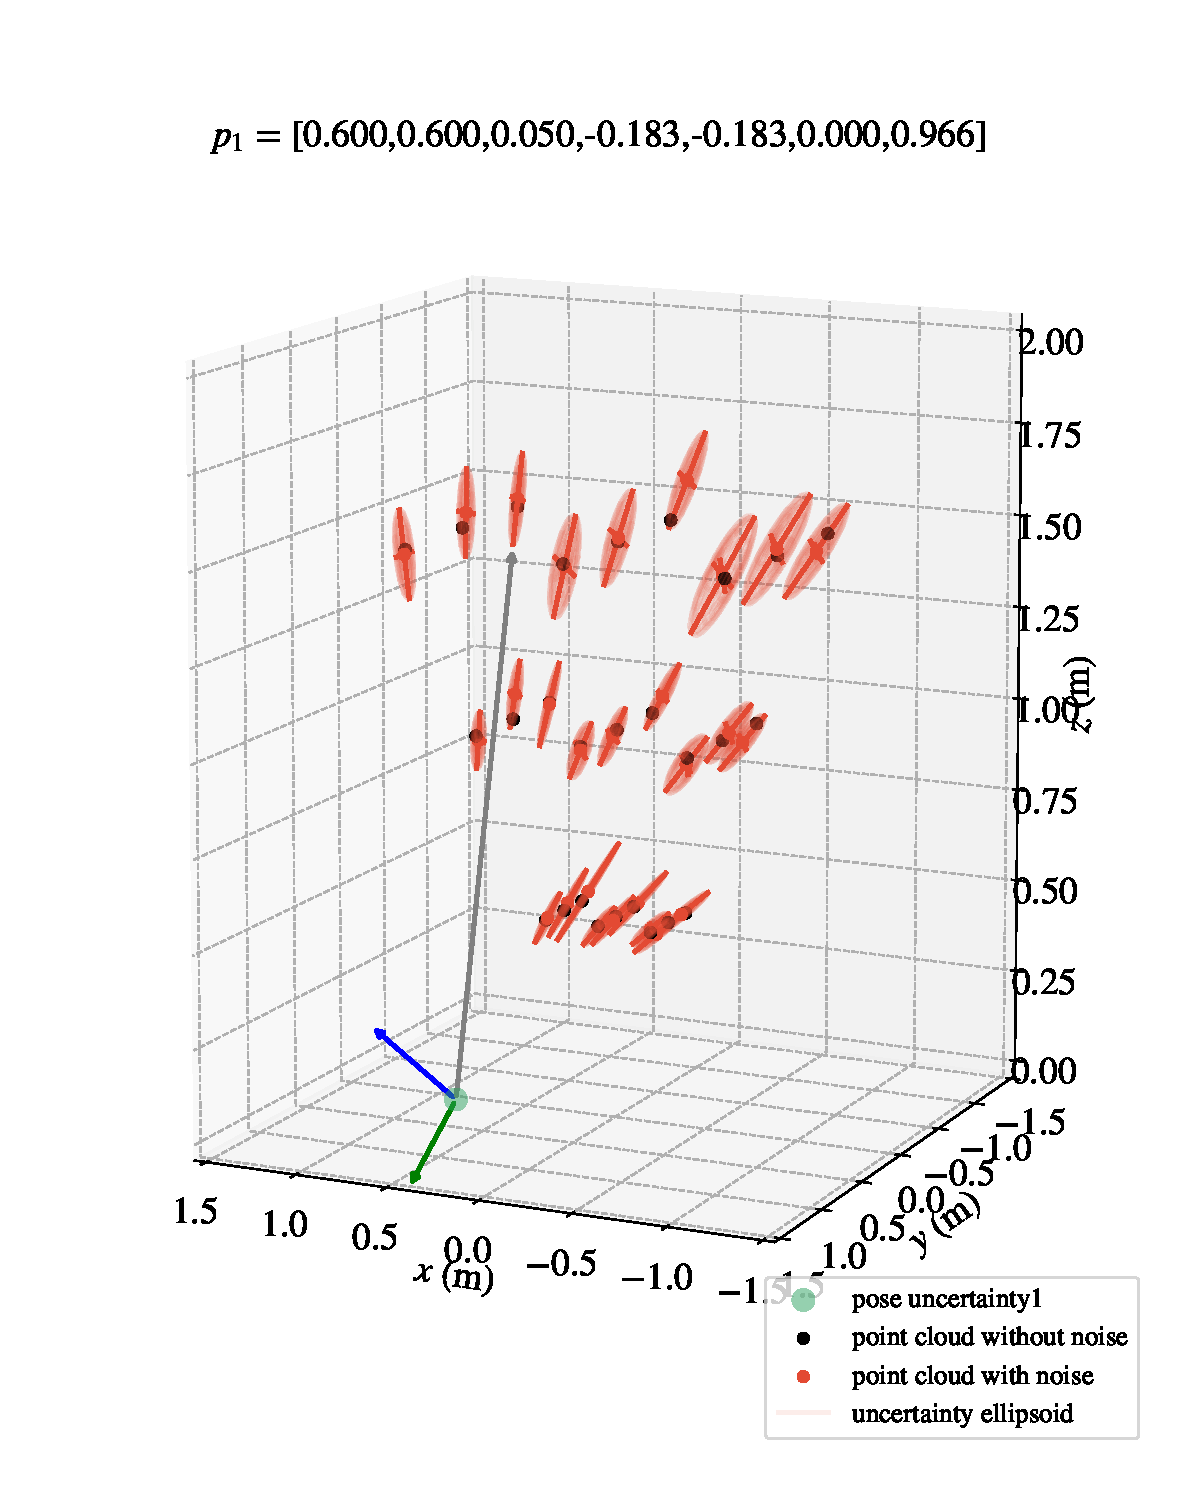
\includegraphics[width=\linewidth,natwidth=640,natheight=640]
  {fig/eva_graphs/sim_at_p1.pdf}
  \caption{asda}
	\label{fig:sim_at_p1}
\end{figure}

Then, we move and rotate the camera to its next pose $p_1$ in the figure 
\ref{fig:sim_at_p1}. Notice how confidence ellipsoids are changed with 
the new camera pose accordingly.


\begin{figure}[H]
  \centering
  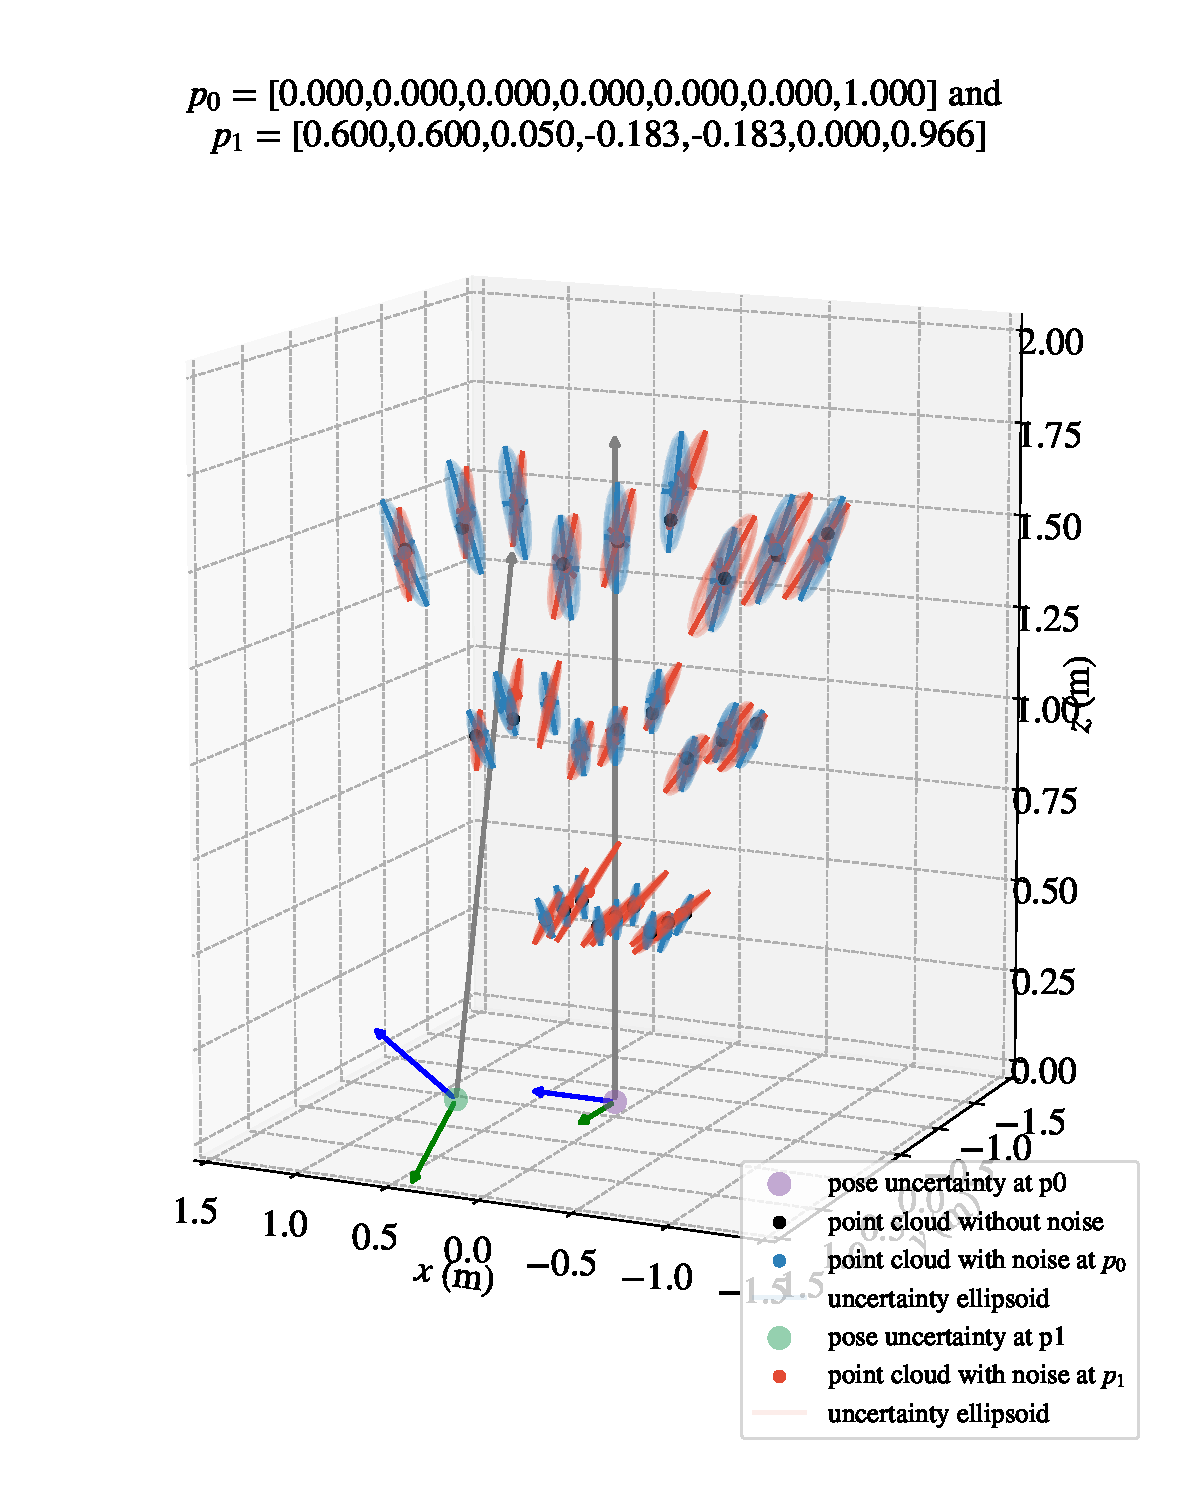
\includegraphics[width=\linewidth,natwidth=640,natheight=640]
  {fig/eva_graphs/sim_at_p0p1.pdf}
  \caption{asda}
	\label{fig:sim_at_p0p1}
\end{figure}

Finally, the figure \ref{fig:sim_at_p0p1} shows how confidence ellipsoids 
from both views intersect each other and include the real feature points within 
the intersected space.

% 4
\subsection{RPE and The Estimated Covariances}

With the simulated data, we estimate relative poses $\mathbf{x^*}_{1:1000}$
and its convariances $\mathbf{x^*}_{1:1000}$. Then, we calculate RPE with 
$\Delta=1$ so that we validate whether the error lies within the 3 sigma bounds
for each parameters of the state vector. 3 sigma bounds corresponds to a rule of 
thumb that expresses 99.7\% probability as near certainty.


% Translation RPE with 3 sigma 
\begin{figure}[H]
  \centering
  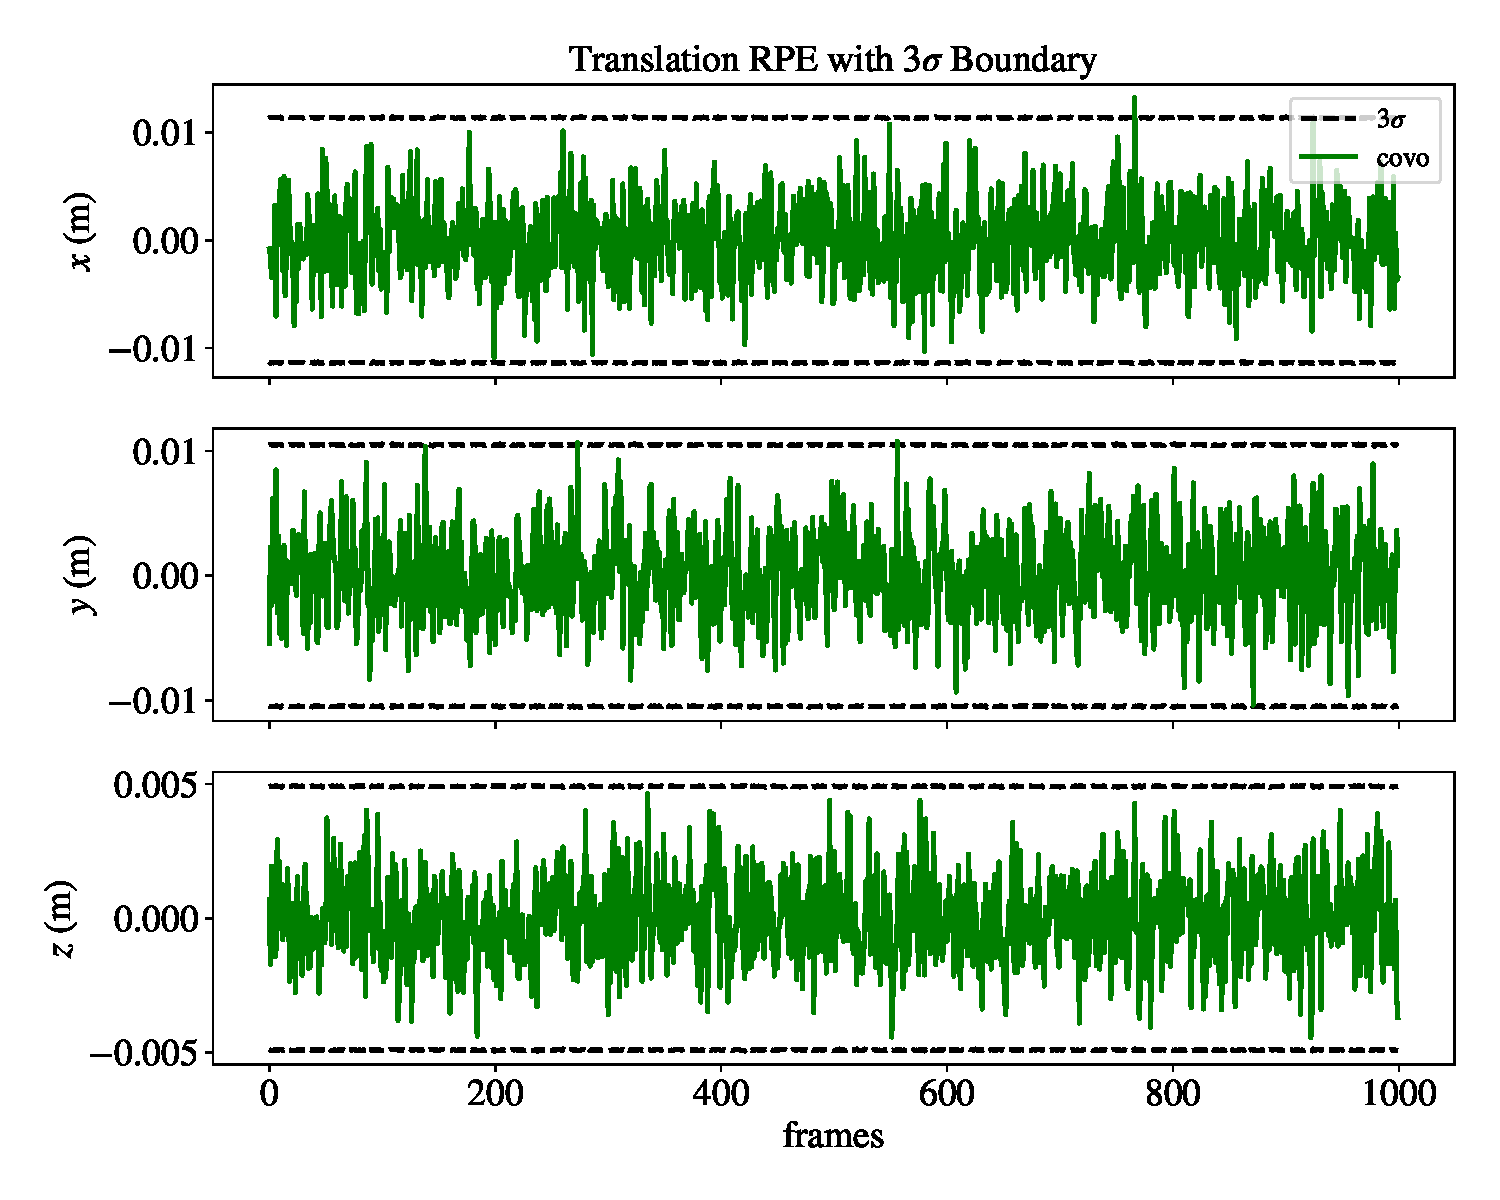
\includegraphics[width=0.8\linewidth,natwidth=640,natheight=640]
  {fig/eva_graphs/synt_trans_rpe_3sigma.pdf}
  \caption{asda}
  \label{fig:synt_trans_rpe_3sigma}
\end{figure}

As seen in figure \ref{fig:synt_trans_rpe_3sigma}, parameters of the translation 
are bounded with 3 sigma with maximum 2 or 3 predictions which is statistically 
acceptable. 

% Rotation RPE with 3 sigma 
\begin{figure}[H]
  \centering
  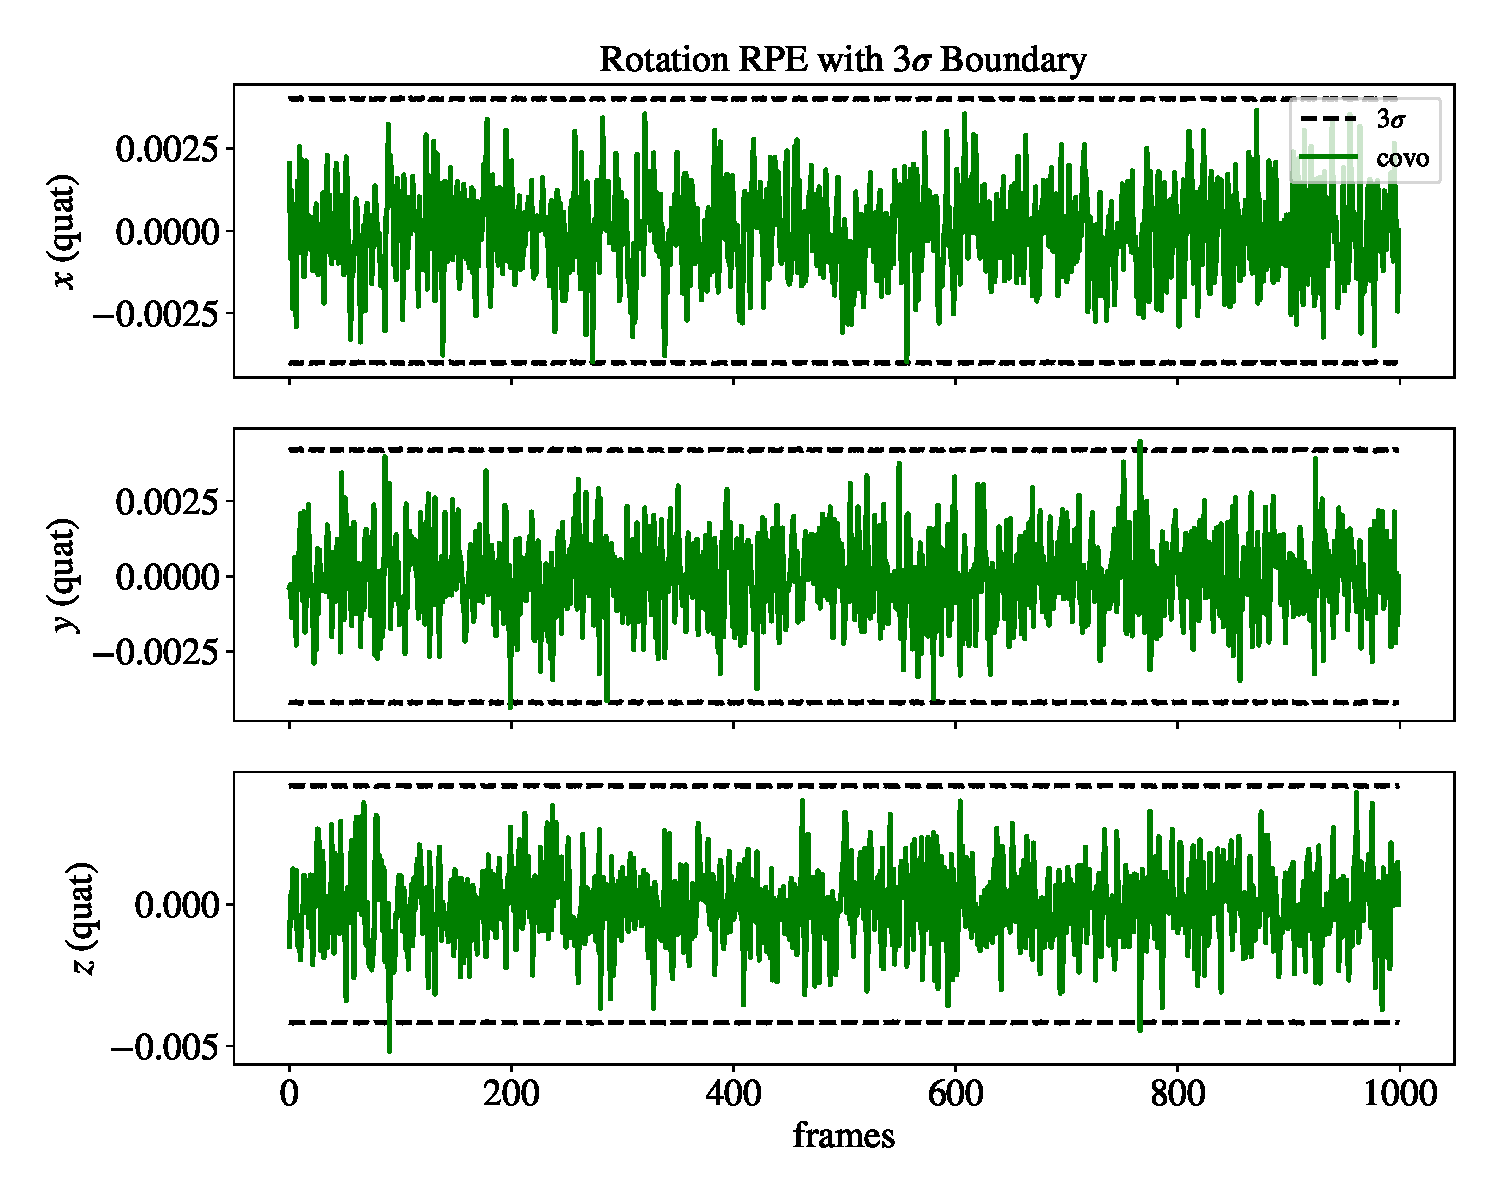
\includegraphics[width=0.8\linewidth,natwidth=640,natheight=640]
  {fig/eva_graphs/synt_rot_rpe_3sigma.pdf}
  \caption{asda}
	\label{fig:2d_local_coords_in_world_coords}
\end{figure}

The same behavior is observed for the rotation as well. This indicates that 
the propagated covariances of the estimated poses based on the 
proposed model produce statistically meaningful uncertainty with simulated data 
if $3\sigma$ bounds are considered. However, $3\sigma$ bounds evaluations itself 
is not enough to prove estimator's credibility. Thus, further evaluations are 
done with NEES.

% 3
\subsection{Evaluation of Estimated Covariances}

Even though $3\sigma$ bounds confirm that our algorithm provides consistent 
pose estimation given RPE is bounded, we need to check whether the 
covariance of the estimated pose are being too optimistic or not.
Hence, we run our simulation as described at the beginning of this section. 
We get ANEES; i.e, 15.64 for translation and 15.72 for rotation. 
We also illustrate the results in figure \ref{fig:test_hist_nees_1}.


\begin{figure}[H]
\begin{tabular}{ccc}
\centering
\subcaptionbox{NEES}{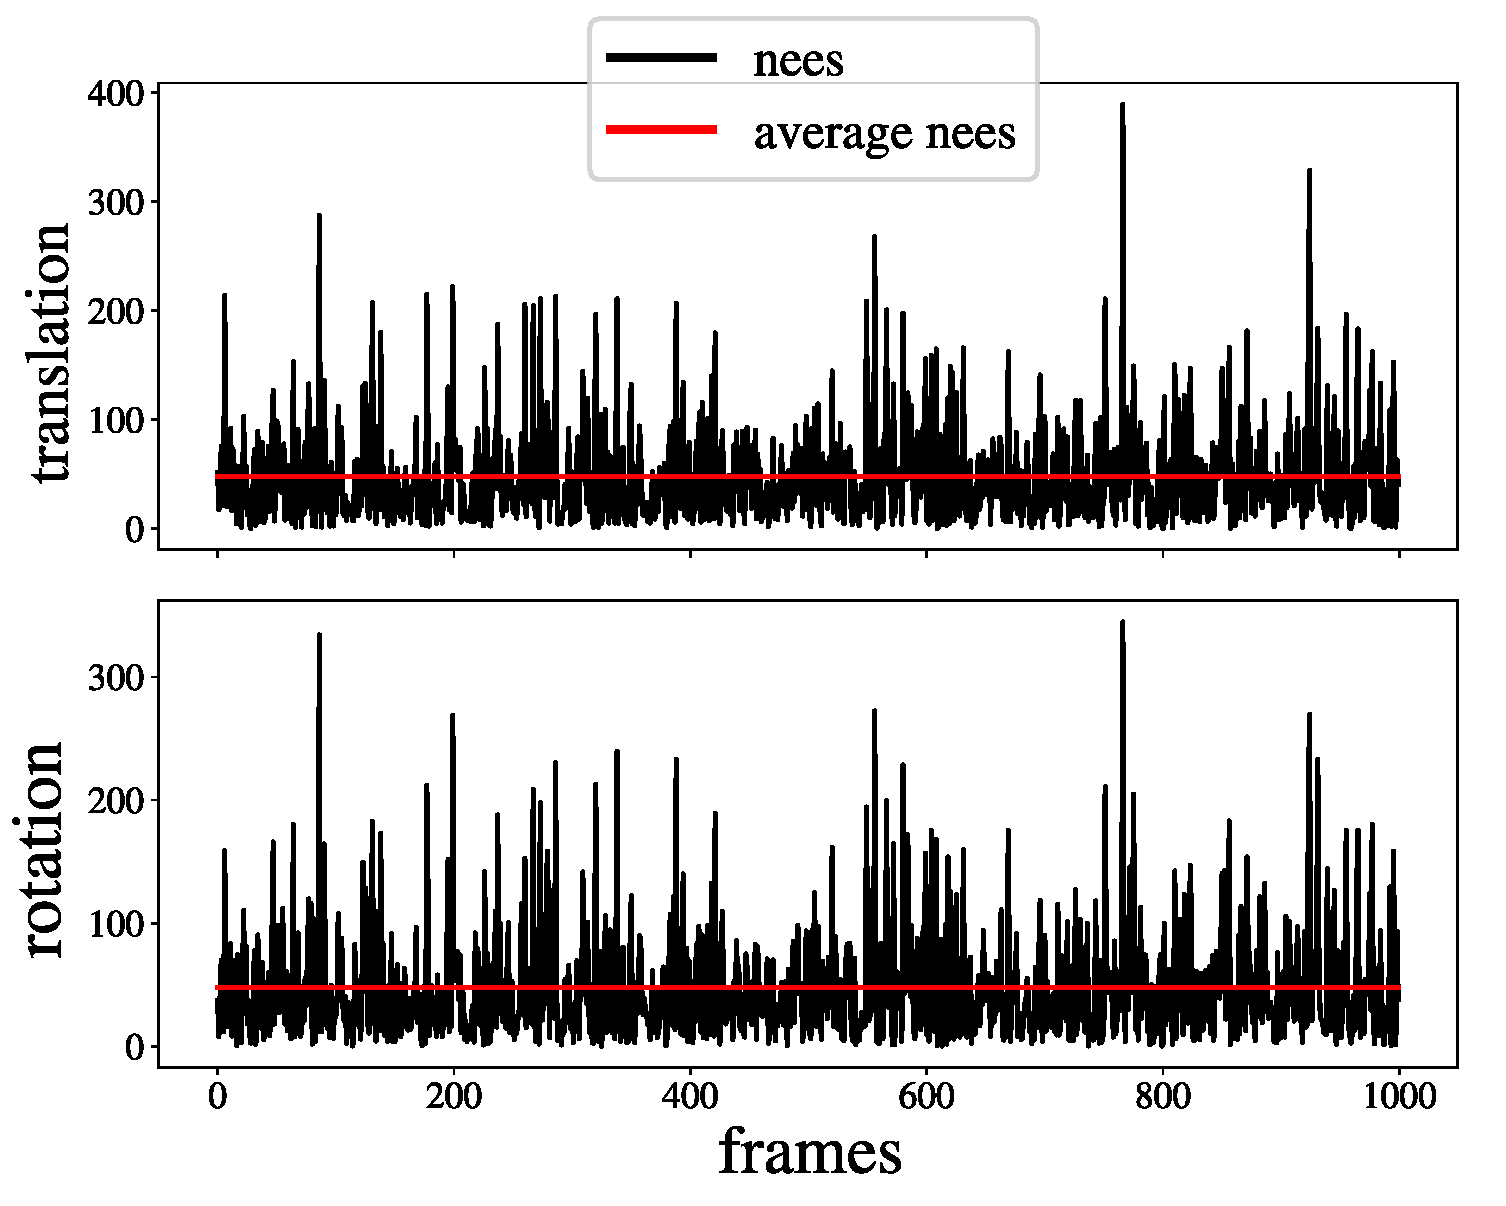
\includegraphics[width = 0.55\linewidth]{fig/eva_graphs/synt_nees.pdf}} &
\subcaptionbox{Histogram of NEES}{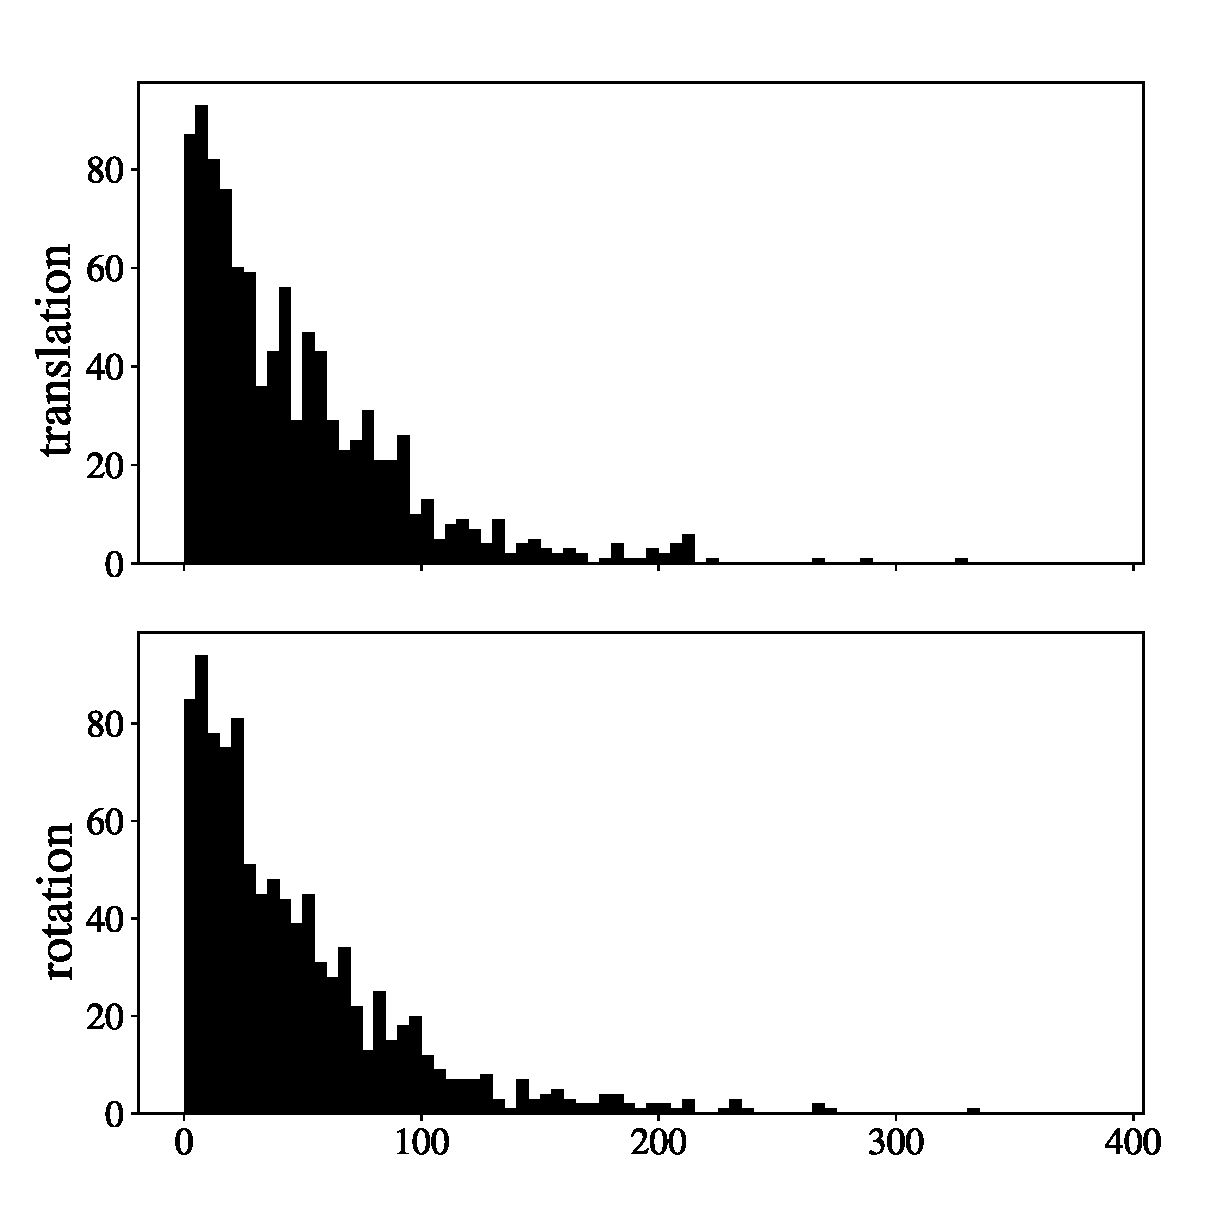
\includegraphics[width = 0.40\linewidth]{fig/eva_graphs/synt_hist_nees.pdf}}
\end{tabular}
\caption{Remove Y axes title and Y axes thick from graphs!!!}
\end{figure}\label{fig:test_hist_nees_1}

%Translation Average NEES: 15.64
%Rotation Average NEES: 15.72

These results show that the estimator is not consistent. This is because 
the projection operation introduces non-linearity to the system and 
we only approximate covariance of 3D feature points with first-order 
taylor expansion. This linearization process does not work well with 
large noises. In this case, [\cite{Shalom2001}, pp.395-397] 
suggests couple of heuristic methods to make the estimator consistent.
Among them, we apply multiplication of estimated covariance $\mathbf{Q_{t,q}}^{(k,k+1)}$
by scaling factor $\phi$ after optimiziton.

\begin{figure}[H]
\begin{tabular}{ccc}
\centering
\subcaptionbox{NEES}{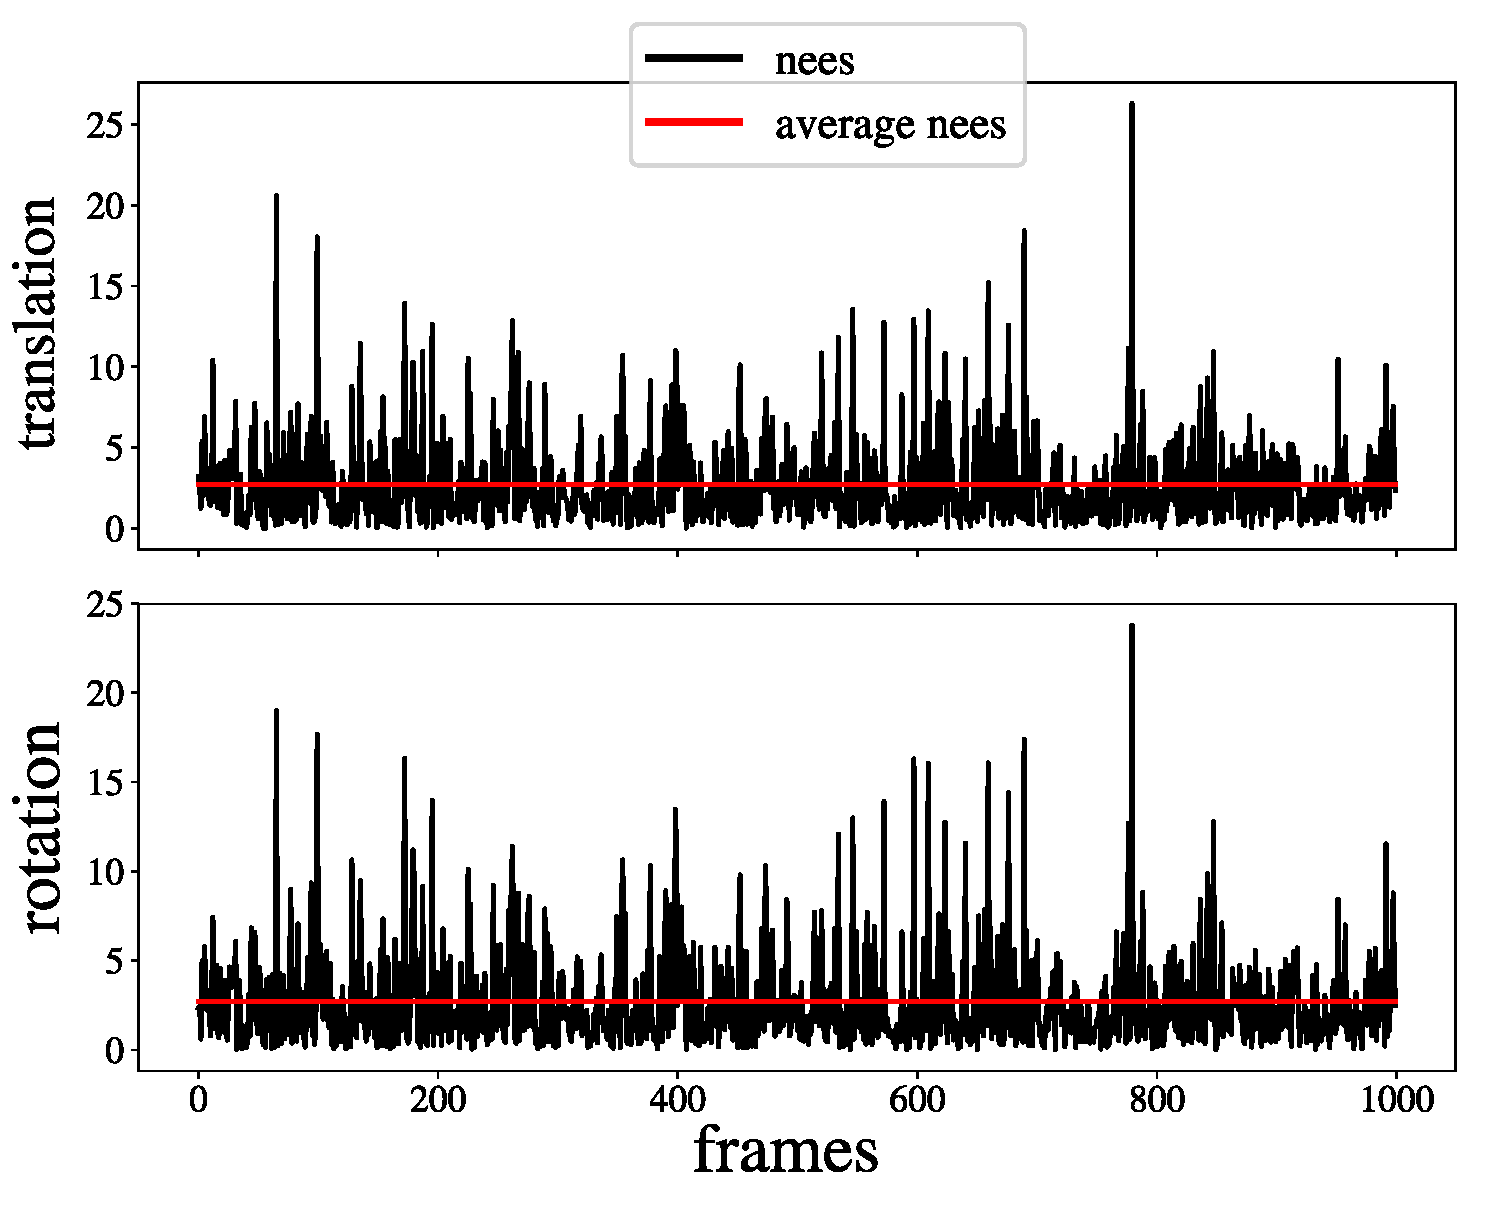
\includegraphics[width = 0.55\linewidth]{fig/eva_graphs/synt_nees_2.pdf}} &
\subcaptionbox{Histogram of NEES}{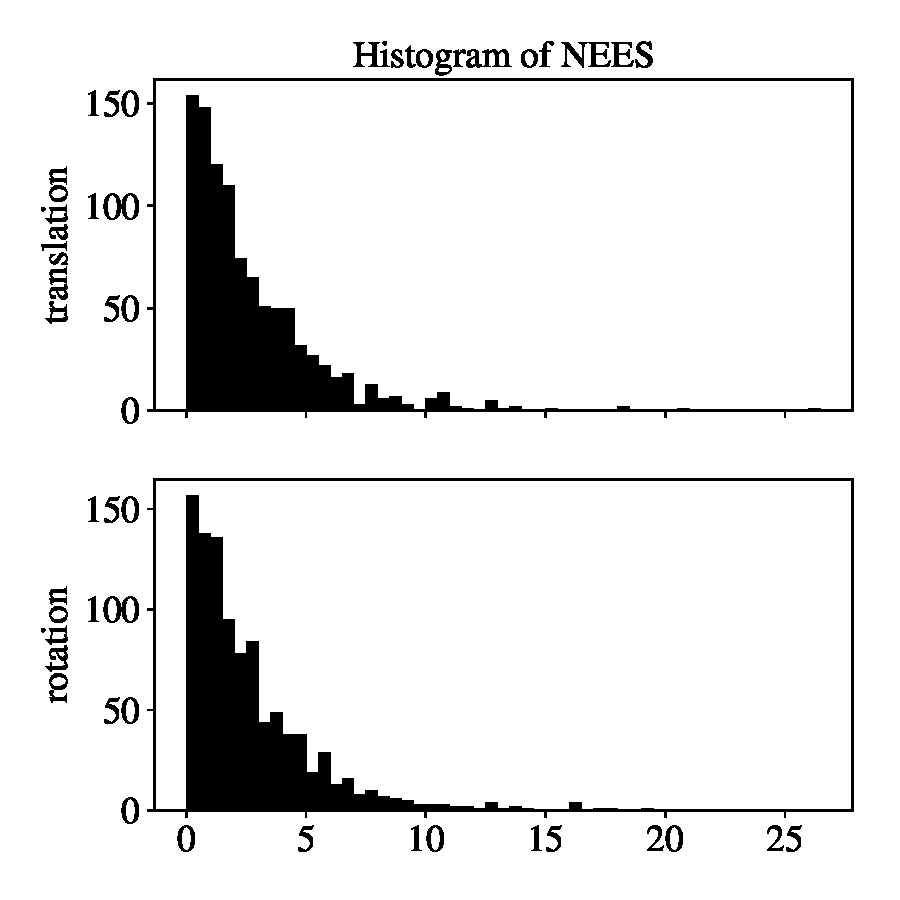
\includegraphics[width = 0.40\linewidth]{fig/eva_graphs/synt_hist_nees_2.pdf}}
\end{tabular}
\caption{Remove Y axes title and Y axes thick from graphs!!!}
\end{figure}\label{fig:test_hist_nees_2}

We find out that ANEES for translation and rotation becomes 2.7 and 2.69, 
respectively when taking $\phi=4^2$ and the results are shown in figure 
\ref{fig:test_hist_nees_2}. These values can be accepted as we consider 
the estimator to be consistent for this setup.

%Translation Average NEES: 2.70
%Rotation Average NEES: 2.69

\section{TUM RGB-D Dataset}

TUM dataset \cite{Sturm2012a} provides an extensive bechmark capability for 
RGB-D based Visual SLAM or VO systems. It consists of datasets that are 
collected in two different indoor environment; i.e, fr1 refers to 
datasets collected in an office $(6\times 6 m^2)$ and fr2 is colleced in an open spaced 
garage $(10\times 12m^2)$. In our experiments, we choose a subset of datasets that are mainly 
suitable for VO and has sufficient texture on the images. 
The selected datasets are given in table \ref{tb:tum_dataset}.
In addition, calibration parameters of RGB and depth images are validated 
by the time-synchronized ground truth measurements recorded by a motion capture system.

\begin{center}
  \begin{tabular}{lccc}
    \hline
    Dataset & Duration & Avg. Trans. & Avg. Rot.\\
     Name & [s] & Vel. [m/s] & Vel. [deg/s]\\
    \hline
    fr1 xyz   & 30 & 0.24 & 8.92\\
    fr1 rpy   & 28 & 0.06 & 50.15\\
    fr1 room  & 49 & 0.33 & 29.88\\
    fr1 360   & 29 & 0.21 & 41.60\\
    fr1 desk  & 23 & 0.41 & 23.33\\
    fr1 desk2 & 25 & 0.43 & 29.31\\
    fr2 desk  & 99 & 0.19 & 6.34\\
    \hline
    \end{tabular}
  \end{center}\label{tb:tum_dataset}

  In the following sections, we will use these datasets to validate 
  our relative pose estimation and its covariance 
  with regards to accuracy and consistency.

\subsection{Discovering Effect of Pseudo Inliers on Pixel Uncertainty}

As discussed earlier in section \ref{sb_sc_pixel_uncertainty}, pixel 
uncertainty caused by quantization operation is treated as half pixel. 
Nevertheless, this error is itself not sufficient when choosing 
standard deviation of pixel noise for covariance of 3D features 
to be propagated through the \ref{} equation. Remember that 
we still had outliers in feature matching even after applying RANSAC, 
which we call them as pseudo inliers. We proposed to treat them as 
inliers, but they will increase the pixel uncertainty. We also assume that 
RANSAC will bound these pseudo inliers. Thus, we are interested in 
determining the boundaries which we will set them as pixel uncertainties 
We determine them using TUM RGB-D and the ground truth measurements.

% Time-based error histogram with 20 frame discrete window
% - Show that pixel errors are gaussian and stds are different along the path

\begin{figure}[H]
  \makebox[\textwidth][c]{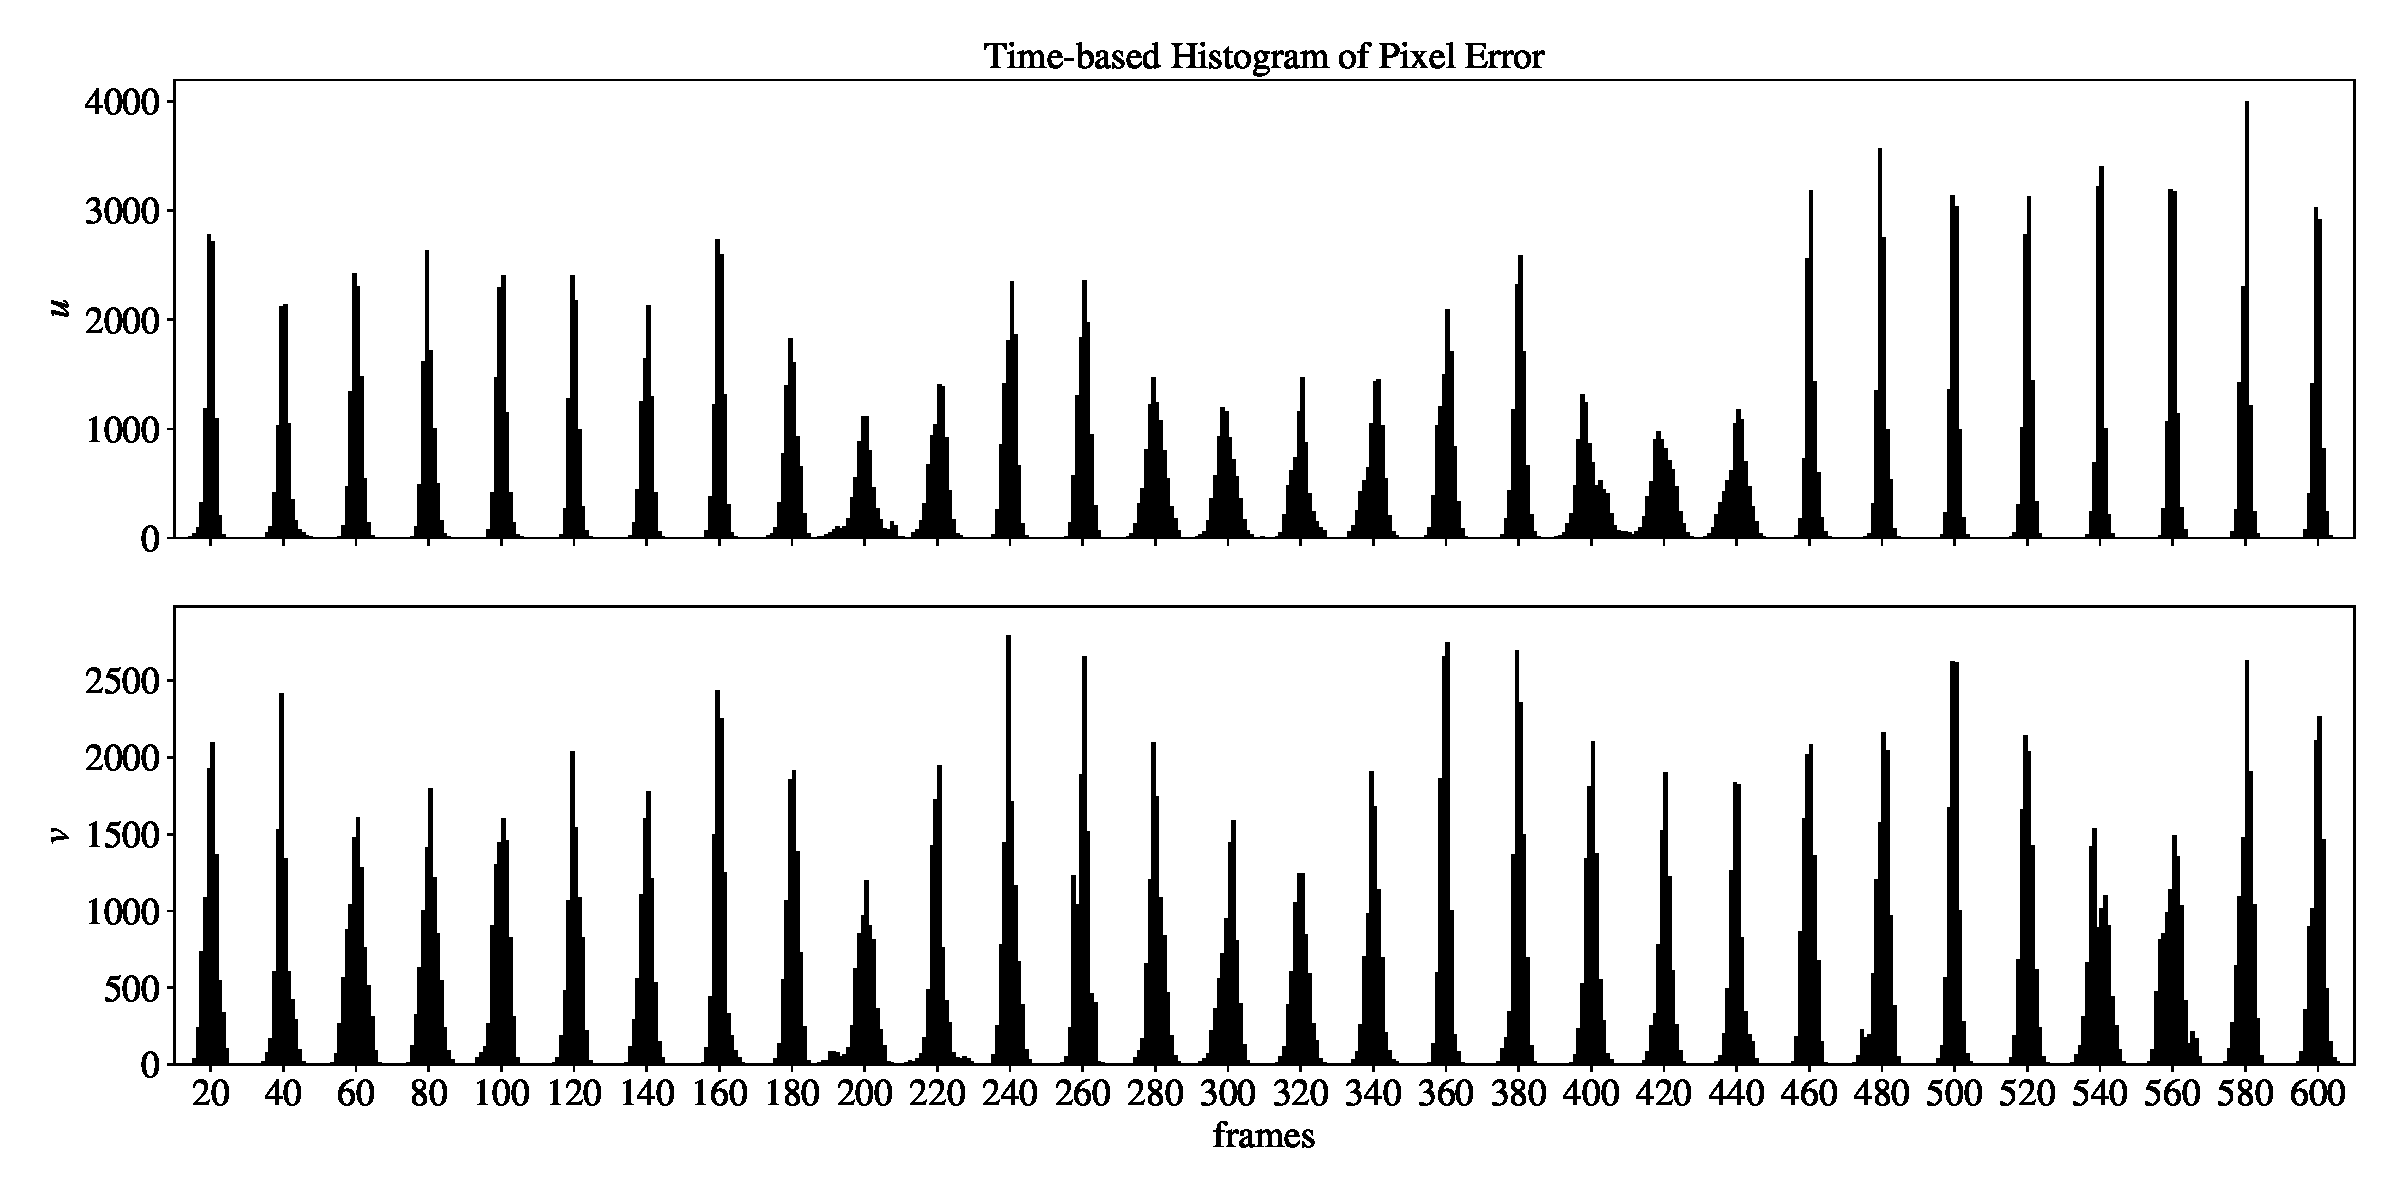
\includegraphics[width=1.4\linewidth,natwidth=640,natheight=640]
  {fig/eva_graphs/tum_fr1_xyz_tbased_hist_uv_err.pdf}}
  \caption{explain the window}
\end{figure}\label{fig:time_based_hist_pix_err}

Let's remind ourselves with the procedures of the pipeline.
To find the pixel error caused by pseudo inliers, we run our VO pipeline 
up until the optimization part estimating the pose. 
To do so, we first extracted features, then matched them and finally filtered outliers with RANSAC. 
At this point, we have feature matches that includes pseudo inliers. 
Now, instead of estimating the relative pose,
we can identify boundaries of the pseudo inliers caused by RANSAC 
by using ground truth data. With using translation and rotation information 
from ground truth, we project features matches one on another. 
Then, for some matches, we expect to get pixel errors to be greater than 1 as 
they are the pseudo inliers.
This test case is applied on every consecutive frame of the whole trajectory.
Next, we illustrate the results in a time-based scheme to observe 
how the pixel error changes throughout the trajectory. The illustration 
gathered by 'fr1 xyz' dataset is given in figure \ref{fig:time_based_hist_pix_err}.
As observed, pixels error mainly caused by pseudo inliers are distibuted as 
gaussian and its standard deviation changes over the trajectory. To 
see how it changes we draw the time-based standard deviation of the pixel errors 
in figure \ref{fig:time_based_std_pix_err}.

NOTE: THERE IS SOMETHING WRONG WITH THE NUMBERING OF FIGS.
% Time-based std with 5 frame sliding window with fr1_xyz

\begin{figure}[H]
  \centering
  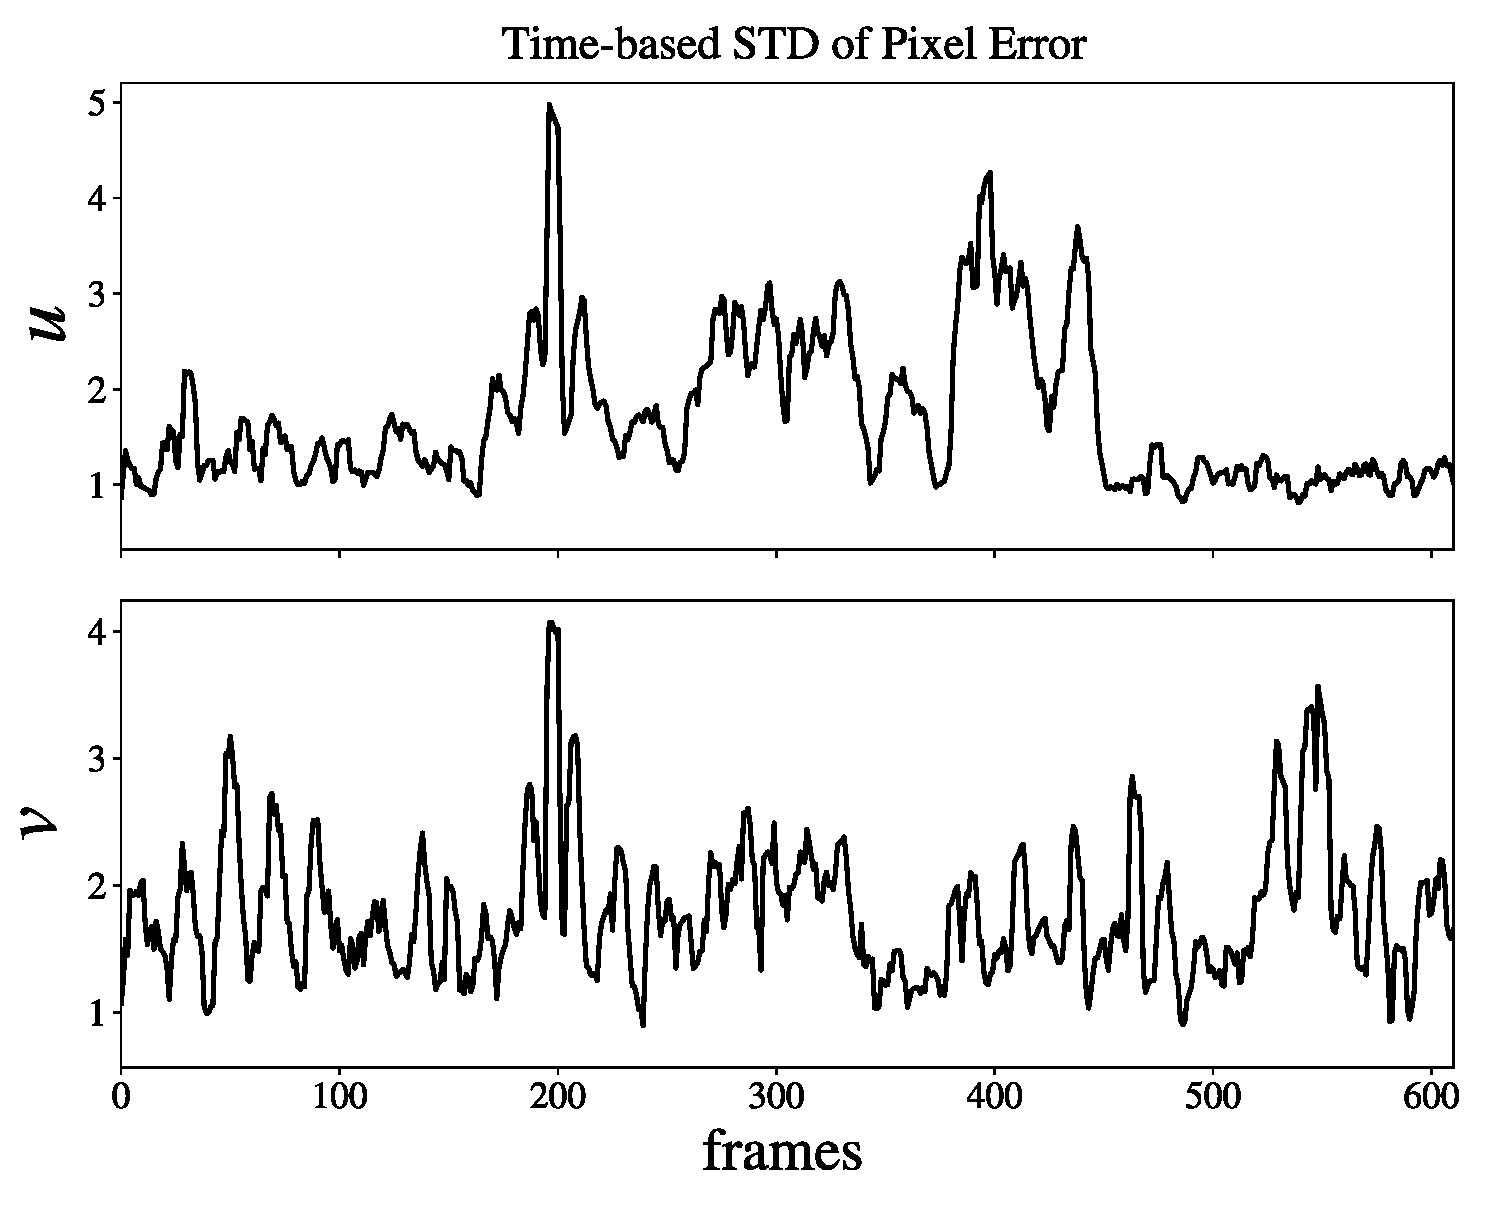
\includegraphics[width=\linewidth,natwidth=640,natheight=640]
  {fig/eva_graphs/tum_fr1_xyz_tbased_uv_err_std.pdf}
  \caption{asda}
\end{figure}\label{fig:time_based_std_pix_err}

The goal is to run this test over many datasets so that we can find the largest 
standard deviation. The result of these test are represented with 
the boxplots in figure \ref{fig:boxplot_time_based_std_all_datasets}.

% Boxplot of Time-based std with 5 frame sliding window for all datasets

\begin{figure}[H]
\begin{tabular}{ccc}
\centering
\subcaptionbox{fr1 xyz}{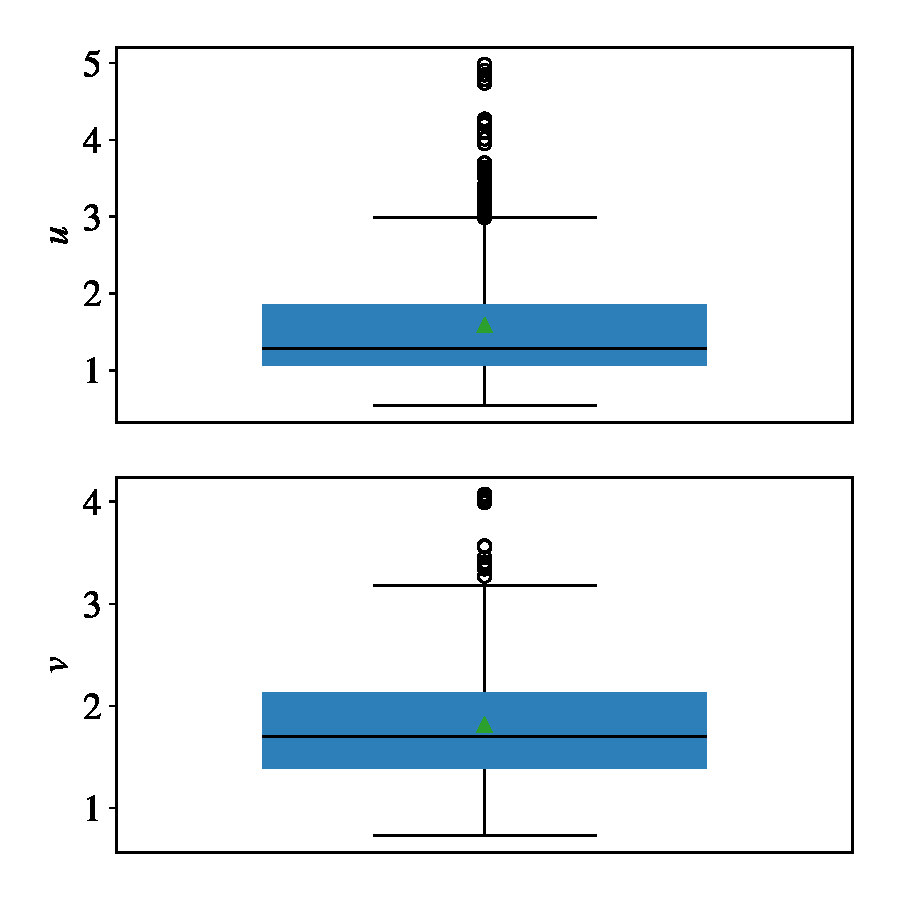
\includegraphics[width = 0.3\linewidth]{fig/eva_graphs/boxplot_tbased_uv_err_std_fr1_xyz.pdf}} &
\subcaptionbox{fr1 rpy}{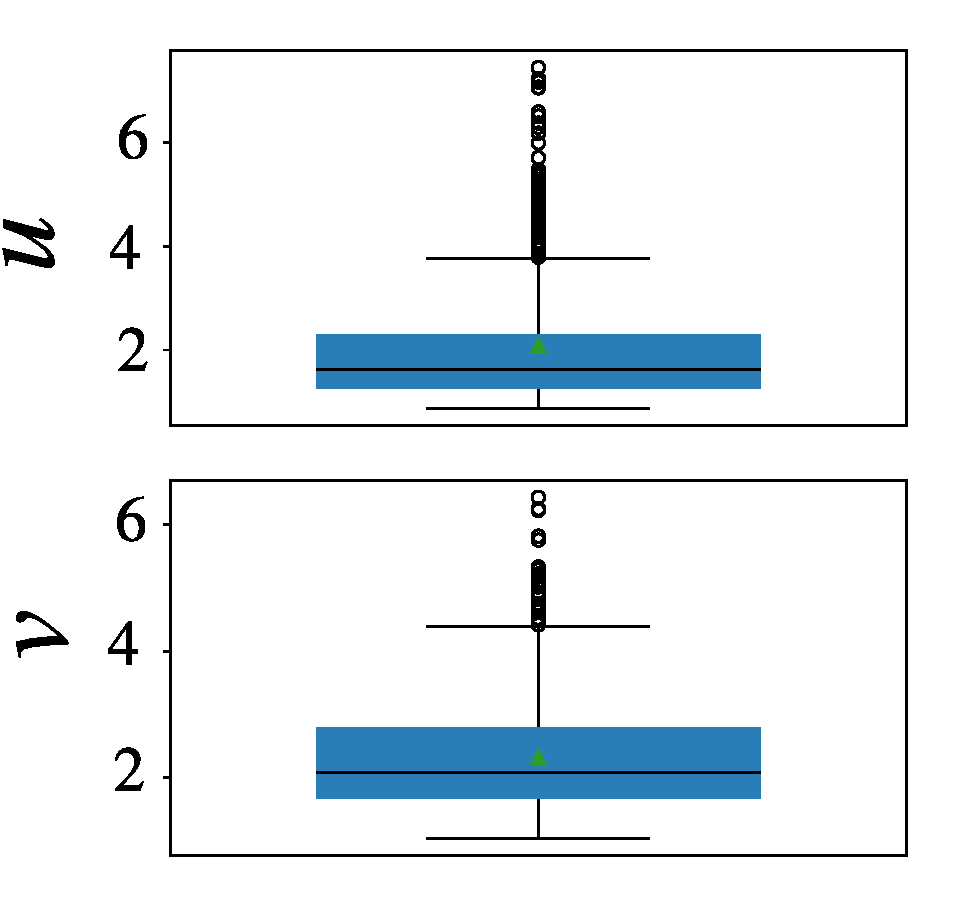
\includegraphics[width = 0.3\linewidth]{fig/eva_graphs/boxplot_tbased_uv_err_std_fr1_rpy.pdf}} &
\subcaptionbox{fr1 room}{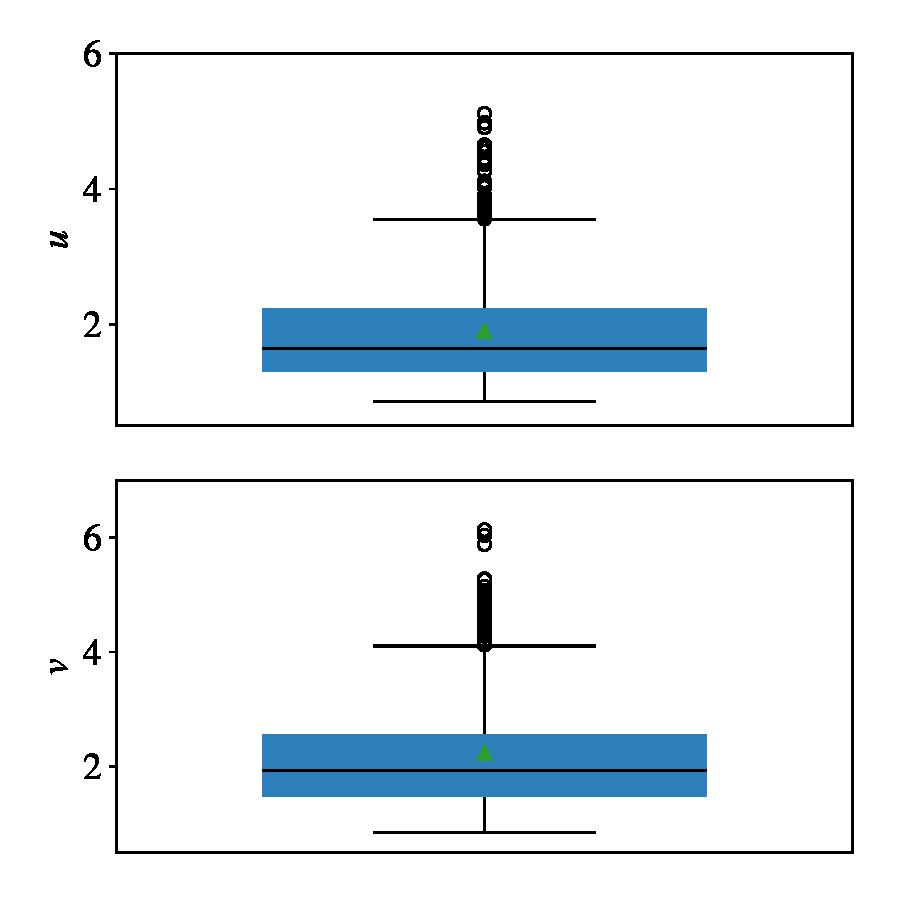
\includegraphics[width = 0.3\linewidth]{fig/eva_graphs/boxplot_tbased_uv_err_std_fr1_room.pdf}} \\
\subcaptionbox{fr1 360}{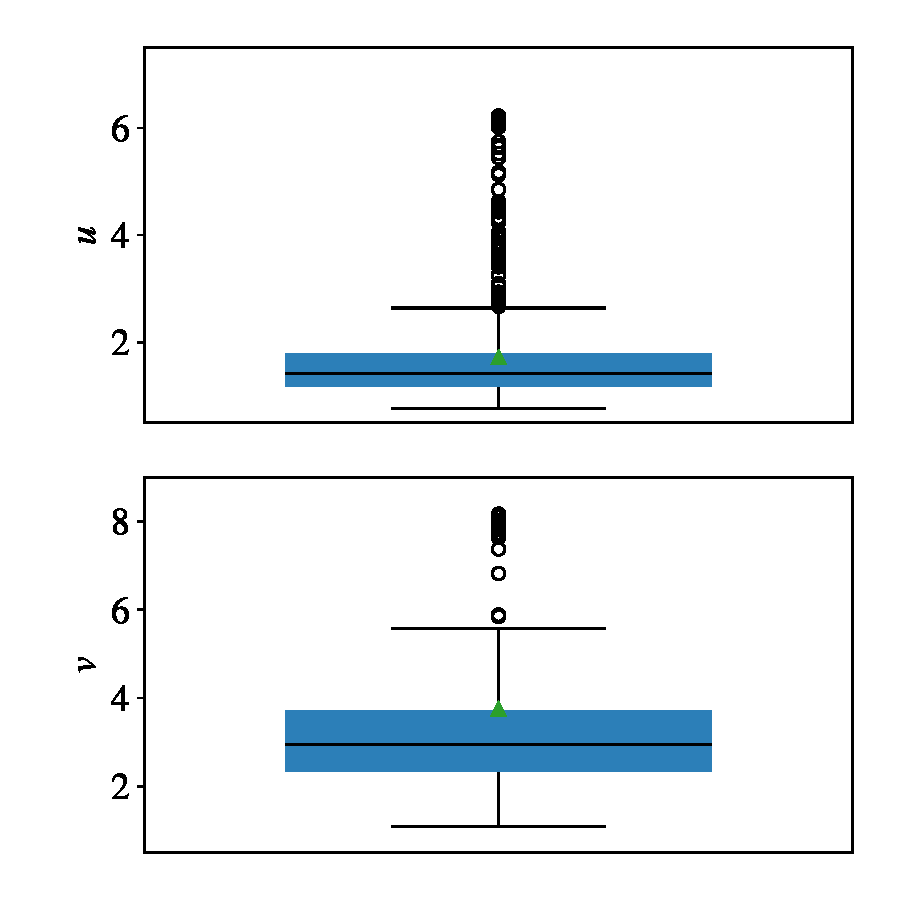
\includegraphics[width = 0.3\linewidth]{fig/eva_graphs/boxplot_tbased_uv_err_std_fr1_360.pdf}} &
\subcaptionbox{fr1 desk}{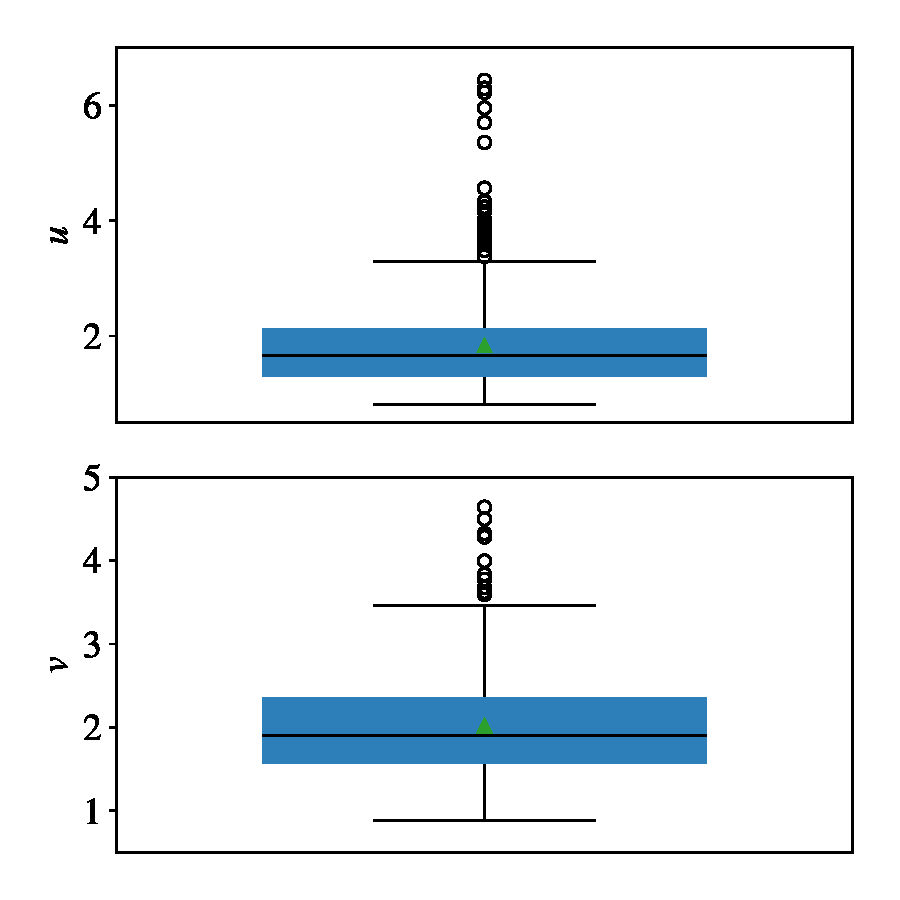
\includegraphics[width = 0.3\linewidth]{fig/eva_graphs/boxplot_tbased_uv_err_std_fr1_desk.pdf}} &
\subcaptionbox{fr1 desk2}{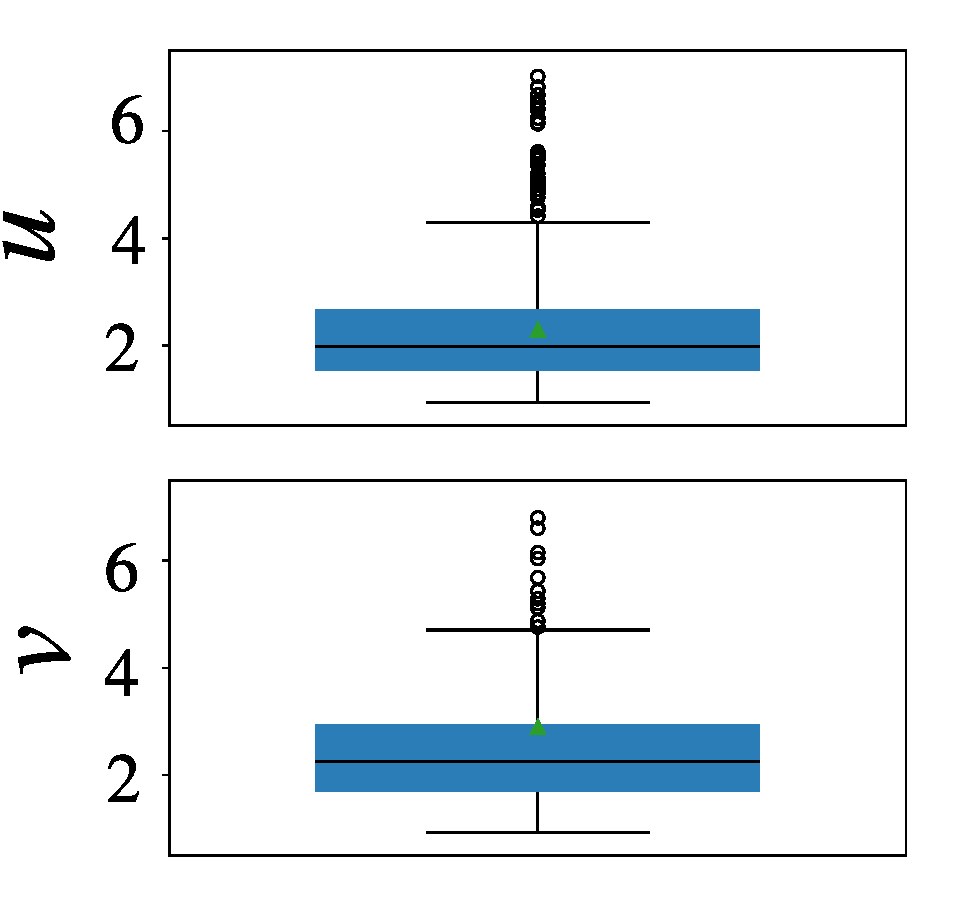
\includegraphics[width = 0.3\linewidth]{fig/eva_graphs/boxplot_tbased_uv_err_std_fr1_desk2.pdf}}
\end{tabular}
\caption{Remove Y axes title and Y axes thick from graphs!!!}
\end{figure}\label{fig:boxplot_time_based_std_all_datasets}

To cover the worst case scenario, 
we take these values as largest value of standard deviations of the pixel noise 
when forming covariance matrix $\mathbf{Q_{uvz}}^{(i,k)}$.

% 2

%\subsection{Estimation of Relative Pose and its Covariance}
%
%% 2.1
%% - Decide which one to use for scaling: RANSAC Threshold or max std?
%% -> DONE! Decided on max std besides the outliers due to wrong ground truth!
%% - Show estimated covariances that is scaled with RANSAC Threshold or Max std?
%
%% Translation RPE frame-to-frame with 3 sigma with fr1_xyz
%\begin{figure}[H]
%  \centering
%  \includegraphics[width=\linewidth,natwidth=640,natheight=640]
%  {fig/eva_graphs/tum_fr1_xyz_trans_rpe_3sigma.pdf}
%  \caption{asda}
%	\label{fig:2d_local_coords_in_world_coords}
%\end{figure}
%
%
%% Rotation RPE frame-to-frame with 3 sigma with fr1_xyz
%\begin{figure}[H]
%  \centering
%  \includegraphics[width=\linewidth,natwidth=640,natheight=640]
%  {fig/eva_graphs/tum_fr1_xyz_rot_rpe_3sigma.pdf}
%  \caption{asda}
%	\label{fig:2d_local_coords_in_world_coords}
%\end{figure}
%

% 1
\subsection{Evaluation of Estimated Covariance}

Similar to simulation data, we calculate NEES for covariance of the estimated 
poses after running the VO algorithm 6 different datasets in TUM. 
Note that we set standard deviation of pixel uncertainty according to 
the largest value $\sigma_u=7$ and $\sigma_v=8$ 
determined in the experimental analysis done in previous section.
After each optimization, we scale resulting covariance $\mathbf{Q_{t,q}}^{(k,k+1)}$
with the $\phi=4^2$ to compensate the errors due to the linearization.
Under these parameterizations, we run the algorithm and calculate 
histogram of NEES and ANEES for the selected datasets. 
The resulting histograms are illustrated in \ref{fig:hist_nees_all_datasets} and 
their ANEES are given in table \ref{tb:anees_all_datasets}.


%% NEES and ANEES with fr1_xyz
%\begin{figure}[H]
%  \centering
%  \includegraphics[width=\linewidth,natwidth=640,natheight=640]
%  {fig/eva_graphs/tum_fr1_xyz_nees.pdf}
%  \caption{asda}
%	\label{fig:2d_local_coords_in_world_coords}
%\end{figure}

% Without average by 3 (degree of freedom)
%fr1 xyz
%Translation Average NEES: 24.102167961194326
%Rotation Average NEES: 52.094722966630314
%fr1 360 
%Translation Average NEES: 23.056611560549662
%Rotation Average NEES: 75.33737874564399
%fr1 rpy 
%Translation Average NEES: 21.70951280913415
%Rotation Average NEES: 64.33137984284465
%fr1 desk
%Translation Average NEES: 60.40113749011506
%Rotation Average NEES: 105.36408125491856
%fr1 desk2
%Translation Average NEES: 56.536957402794926
%Rotation Average NEES: 110.9844039603292
%fr1 room 
%Translation Average NEES: 19.81107198582873
%Rotation Average NEES: 55.49945876186048

% Histogram of NEES with all datasets!
% BUG: Caption does not located under figures!
\begin{figure}[H]
\begin{tabular}{ccc}
\centering
\subcaptionbox{fr1 xyz}{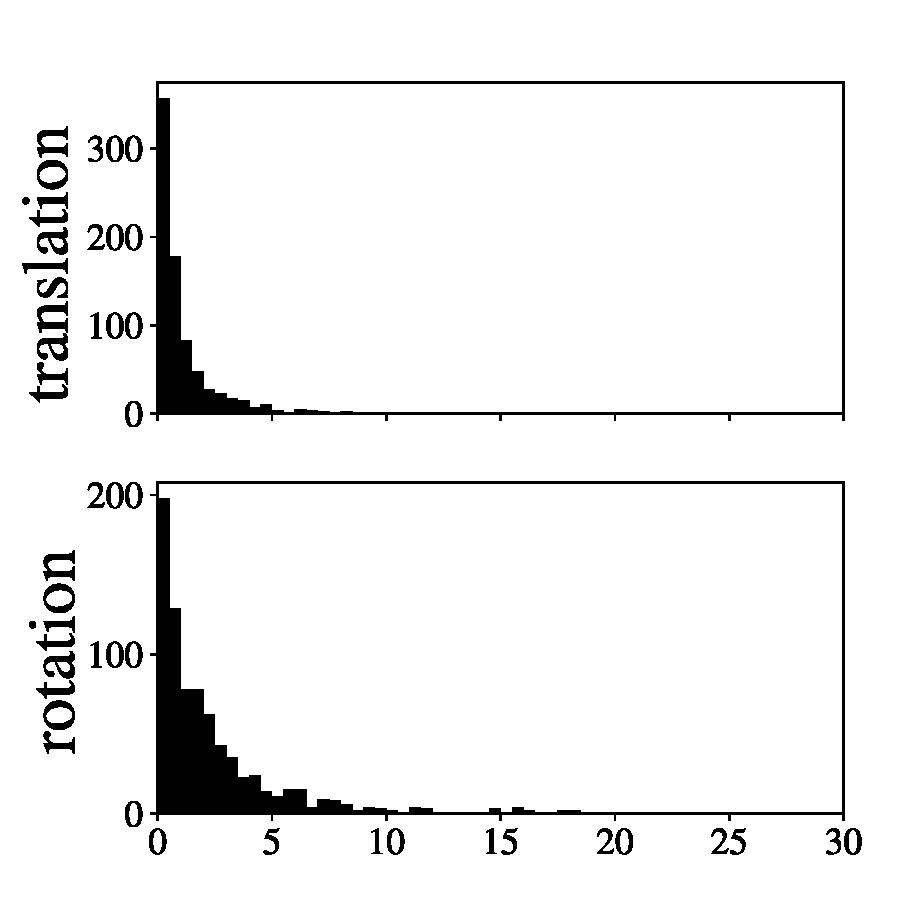
\includegraphics[width = 0.3\linewidth]{fig/eva_graphs/tum_fr1_xyz_hist_nees.pdf}} &
\subcaptionbox{fr1 rpy}{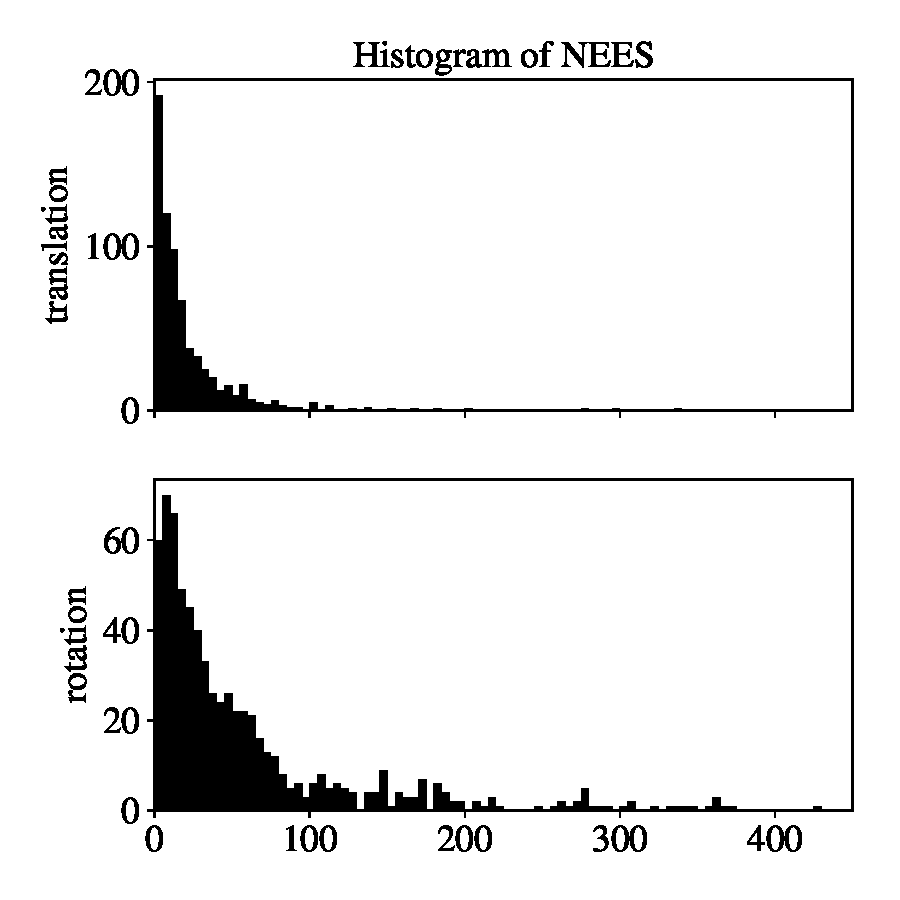
\includegraphics[width = 0.3\linewidth]{fig/eva_graphs/tum_fr1_rpy_hist_nees.pdf}} &
\subcaptionbox{fr1 room}{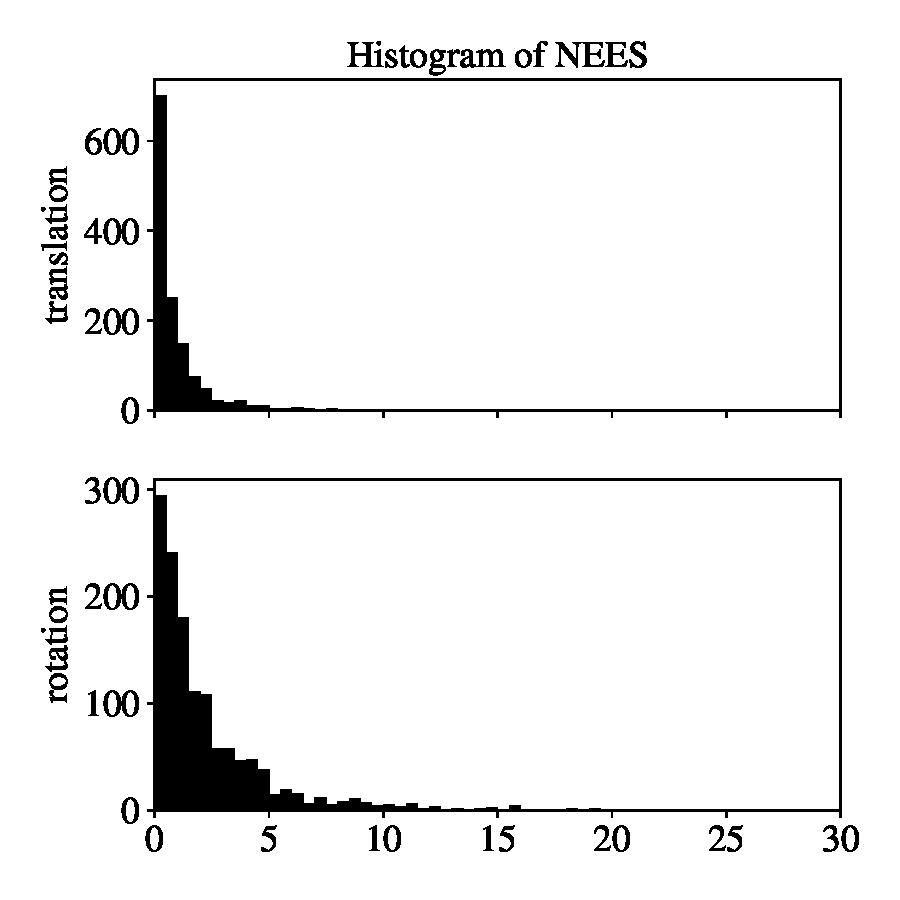
\includegraphics[width = 0.3\linewidth]{fig/eva_graphs/tum_fr1_room_hist_nees.pdf}} \\
\subcaptionbox{fr1 360}{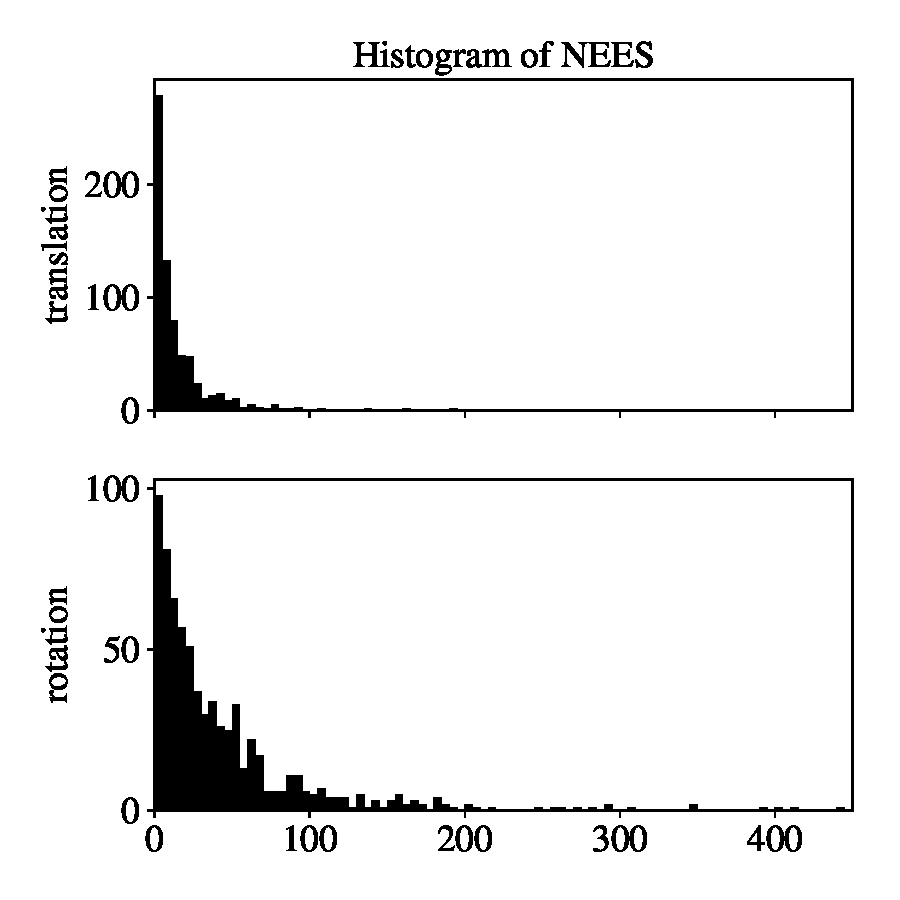
\includegraphics[width = 0.3\linewidth]{fig/eva_graphs/tum_fr1_360_hist_nees.pdf}} &
\subcaptionbox{fr1 desk}{\includegraphics[width = 0.3\linewidth]{fig/eva_graphs/tum_fr1_desk_hist_nees.pdf}} &
\subcaptionbox{fr1 desk2}{\includegraphics[width = 0.3\linewidth]{fig/eva_graphs/tum_fr1_desk2_hist_nees.pdf}}
\end{tabular}
\caption{4 x 4}
\end{figure}\label{fig:hist_nees_all_datasets}

We observe that covariance of the translation estimations are conversative, 
which is acceptable in VO systems. However, covariance of the rotation estimation 
result in being overconfident for 3 datasets; i.e., 'fr1 360', 'fr1 desk' and 'fr1 room'.
Thus, we can say the estimator is \textit{inconsistent} for the rotation, 
as opposed to the translation providing consistent covariance estimations.

\begin{center}
  \begin{tabular}{l|cc|cc}
    \hline
  & Translation ANEES & Status & Rotation ANEES & Status \\
  \hline
  fr1 xyz   & 1.55 & conservative & 2.48 & conservative \\
  \hline
  fr1 rpy   & 1.08 & conservative & 3.10 & conservative \\
  \hline
  fr1 360   & 1.21 & conservative & 3.69 & overconfident \\
  \hline
  fr1 desk  & 2.88 & conservative & 4.99 & overconfident \\
  \hline
  fr1 desk2 & 2.72 & conservative & 5.30 & overconfident \\
  \hline
  fr1 room  & 0.96 & conservative & 2.65 & conservative \\
  \hline
  \end{tabular}
\end{center}\label{tb:anees_all_datasets}


% 5
\section{Comparison to FOVIS}

%subsection{Trajectory Estimation}
As for the accuracy of the estimated poses, we compare the proposed algorithm 
with FOVIS, which is a defacto VO application since it produces very accurate 
pose estimation with fast computations.
To provide an illustration as to building trajectory from relative pose estimations, 
we draw estimations results of 'fr2 desk' which is suitable to present drift effects 
and it is given in \ref{fig:comp_fr2_desk} along with the boxplot representation
of RPEs. 

% Traj XYZ with fr2_desk Boxplot with fr2_desk
\begin{figure}[H]
\begin{tabular}{ccc}
\centering
\subcaptionbox{asd}{\includegraphics[width = 0.5\linewidth]{fig/eva_graphs/fovis_comp_3d_tum_fr2_desk.pdf}} &
\subcaptionbox{asd}{\includegraphics[width = 0.45\linewidth]{fig/eva_graphs/fovis_comp_boxplot_tum_fr2_desk.pdf}}
\end{tabular}
\caption{Remove Y axes title and Y axes thick from graphs!!!}
\end{figure}\label{fig:comp_fr2_desk}

We run both algorithm for the 7 datasets and the resulting RMSEs of RPEs 
are given in table \ref{tb:comp_all_dataset}. Note that we take $\Delta=30$ 
frames while calculating RPEs.

\begin{figure}[H]
\begin{tabular}{ccc}
\centering
\subcaptionbox{fr1 xyz}{\includegraphics[width = 0.3\linewidth]{fig/eva_graphs/fovis_comp_boxplot_tum_fr1_xyz.pdf}} &
\subcaptionbox{fr1 rpy}{\includegraphics[width = 0.3\linewidth]{fig/eva_graphs/fovis_comp_boxplot_tum_fr1_rpy.pdf}} &
\subcaptionbox{fr1 room}{\includegraphics[width = 0.3\linewidth]{fig/eva_graphs/fovis_comp_boxplot_tum_fr1_room.pdf}} \\
\subcaptionbox{fr1 360}{\includegraphics[width = 0.3\linewidth]{fig/eva_graphs/fovis_comp_boxplot_tum_fr1_360.pdf}} &
\subcaptionbox{fr1 desk}{\includegraphics[width = 0.3\linewidth]{fig/eva_graphs/fovis_comp_boxplot_tum_fr1_desk.pdf}} &
\subcaptionbox{fr1 desk2}{\includegraphics[width = 0.3\linewidth]{fig/eva_graphs/fovis_comp_boxplot_tum_fr1_desk2.pdf}}
\end{tabular}
\caption{4 x 4}
\end{figure}


\begin{center}
  \begin{tabular}{lcc}
    \hline
    & FOVIS & COVO\\
     & RMSE & RMSE\\
    \hline
    fr1 xyz   & 0.0240  & 0.0512\\ 
    \hline
    fr1 rpy   & 0.0533  & 0.0368\\
    \hline
    fr1 360   & 0.0867  & 0.1239\\ 
    \hline
    fr1 desk  & 0.0406  & 0.0665\\
    \hline
    fr1 desk2 & 0.0533  & 0.0941\\
    \hline
    fr1 room  & 0.0587  & 0.0791\\
    \hline
    fr2 desk2 & 0.0156  & 0.0428 \\
    \hline
  \end{tabular}\label{tb:comp_all_dataset}
\end{center}

We can say that FOVIS is more accurate than the proposed algorithm and 
name number of reasons. FOVIS utilizes the keyframe scheme and different 
outlier rejection algorithm than RANSAC and 
provides a better initial guess to its optimizer after several refinement processes 
throughout the pipeline.





\chapter{Conclusion} \label{cp_conc}

% what&how I did in 2-3 sent

This thesis was undertaken to design
an error-aware RGB-D Visual Odometry system and evaluate its credibility. 
This achieved by identifying the errors occuring in both sensor 
and algorithm level and integrating them into the optimization 
problem.

% outline thesis
After an introduction chapter, the first step was to lay out 
the foundational elements of Visual Odometry.
% camera model
Then, the geometrical models of a RGB-D camera sensor was given 
in order to be acquainted with the working principles of such sensors 
in Chapter 2. 
The pinhole and triangulation models 
served as essential tools when modeling error characteristics of the sensors.
% typical vo pipeline
In Chapter 3, the typical pipeline of a feature based VO 
was studied. The pipeline comprised of 4 fundamental processes; that is, 
extracting features, matching features, rejecting outliers and 
pose estimation. To model uncertainy of the complete system, 
not only the systematic errors of the sensors, but also 
the errors introduced by the image processing processes are 
needed to be investigated.

% modeling uncertainties of RGB-D
After stating the motivation behind the thesis in Chapter 4, two main source of errors 
are discussed in Chapter 5; i.e., feature related errors caused by outliers and 
depth related errors caused by the IR sensor.  
All of these errors were combined in the conic ray model to 
represent the uncertainty of 3D feature points with covariances.
% optimization 
Afterwards, how these uncertainties were incorporated 
into the optimization process and 
the covariance of the estimated pose was propagated through 
feature uncertainty were described in detail.

% evaluation 
Chapter 6 started with presenting the simulation environment whose purpose 
is to validate the corectness of the algorithm.
% sim 
Experiments in simulation showed that linearization
of projection function led to inconsistency for the covariance 
of the estimated poses in the case of large noise. 
This issue was compensated with a heuristic method that 
scales resulting covariance accordingly.
% tum dataset
Next, TUM RGB-D dataset was used 
not only for testing 
consistency of the estimations with the real-world data, 
but also for identifying the effect of pseudo inliers 
on pixel uncertainty. 
% fovis comp
At the end of the chapther, 
accuracy of the proposed algorithm was compared with FOVIS.

% limitations
Finally, several limitations to this work need to be acknowledged. 
The simulation environment was built under the assumption that the 
pixel and depth uncertainties are gaussian and there are no outliers in 
feature matches. The fact that RANSAC is non-deterministic 
causes to remain outliers that are greater than its acceptance 
threshold. Once remaining outliers are treated as pseudo inliers, 
pixel uncertainty grows, which then brings out issues in the linearizations.
It is also obvious that setting the pixel uncertainty 
by the largest standard deviation value
after running exhaustive tests 
to determine how pseudo inliers' error are distributed throughout all trajectories 
will not cover every corner cases. Thus, this problem requires more 
sophisticated approaches.
In contrast to our simulation environment, 
the analysis being done for estimator's consistency with NEES 
is usually performed in Monte Carlo simulation to introduce greater uncertainty 
to the system.

TODO: open questions and future work

\chapter{Bibliography} \label{cp_bib}

%deleting auto-generated reference title

% throws error
%\renewcommand\refname{\vskip -1cm} 

\nocite{*}

\bibliographystyle{alpha}
\bibliography{/home/bolatu/Documents/mendeley_bib/Master_Thesis_Bib}



% ***************************CP7-EVALUATION***************************
\chapter{Appendices} \label{cp_appendices}

\section{Rigid-Body Transformations} \label{sc_rigid_body_transformations}

\subsubsection{Translation}

\begin{figure}[H]
\begin{tabular}{ccc}
\centering
\subcaptionbox{p0}{\includegraphics[width = 0.45\linewidth]{fig/eva_graphs/append_p0.pdf}} &
\subcaptionbox{p1}{\includegraphics[width = 0.45\linewidth]{fig/eva_graphs/append_p1_trans.pdf}}
\end{tabular}
\caption{}
\end{figure}\label{fig:}


\subsubsection{Rotation with Quaternions}

\begin{figure}[H]
\begin{tabular}{ccc}
\centering
\subcaptionbox{p0}{\includegraphics[width = 0.45\linewidth]{fig/eva_graphs/append_p0.pdf}} &
\subcaptionbox{p1}{\includegraphics[width = 0.45\linewidth]{fig/eva_graphs/append_p2_rot.pdf}}
\end{tabular}
\caption{}
\end{figure}\label{fig:}


\subsubsection{Transformation}

\begin{figure}[H]
\begin{tabular}{ccc}
\centering
\subcaptionbox{p0}{\includegraphics[width = 0.45\linewidth]{fig/eva_graphs/append_p0.pdf}} &
\subcaptionbox{p1}{\includegraphics[width = 0.45\linewidth]{fig/eva_graphs/append_p3_trans_rot.pdf}}
\end{tabular}
\caption{}
\end{figure}\label{fig:}




\section{Least Squares}\label{sc_least_squares}

Throughout this thesis, least squares method empowered many different components 
of out VO system, 
such as camera calibration, RANSAC and most importantly motion estimation, 
Therefore, we will discuss underlying principles of least squares method in this section.

Ultimately, error minimization is an 
operation which wish to get the maximum likelihood of the function. To do so,
we search the most
likely state configuration as close as possible to its exact and ideal solution. 
In the case of any optimization problems,
the goal is to find interesting points, such as local/global
maximum or local/global minimum, on the \textit{objective}
\textit{function}. However, the exact model $F(\mathbf{x})$ of a system 
mostly unknown due to the high-degree for non-linearty or lack of knowledge.
Additionally, one needs to model the noise characteristics of measurements 
in real-world. This noise modeling also requires an approximation. 
Thus, one can only (hopefully) find a good enough solution by iteratively searching.
One way to solve effectively such problems is to generate a quadratic model of 
the objective function around initial guess $\mathbf{x}^0$ and iterate
through the function using the \textit{Newton's methods} or its variations.
For example,
an optimal solution (or an interest point)
Figure-\ref{fig:lsq_multivariable_function_example} is at the local
minimum of the function that is highlighted as a red point cloud.

\begin{figure}[H]
	\centering
	\includegraphics[width=\linewidth,natwidth=640,natheight=640]
	{fig/lsq_multivariable_function_example.jpg}
	\caption{Local Minimum at a Quadratic Function}
	\label{fig:lsq_multivariable_function_example}
\end{figure}


%In optimization literature,
%there are many versions of Newton's method 
%and they all try to find the
%local maximum/minimum in the most efficient and accurate way.

%However, in the end, they all solve the problem
%with the \textit{gradient descent} manner.
%the approximated Hessian function, is one of them and we will be using
%it in our slam algorithm.

To elaborate the problem, we provide a regression example 
which can be infact solved with linear least squares techniques but it can serve 
as a simple toy example throughout our explainations.

Suppose that we have a model function $g(\mathbf{x};a)$. However,
we don't know what the $\mathbf{x}=(x_1,x_2)$ coefficients (so-called
\textit{optimization} \textit{parameters}) are and we can only
plug $a$, which is the \textit{independent} variable, into the
\textit{model} $S$ to see
how the output of the model changes given the independent variable. 

\begin{figure}[H]
	\includegraphics[width=0.8\linewidth,natwidth=640,natheight=640]
	{fig/lsq_model.jpg}
	\centering
	\caption{Least Square Model}
	\label{fig:lsq_model}
\end{figure}



\begin{gather}
\xi = a \text{ (independent variable)} \in \R \\
\eta = S \text{ (dependent variable)} \in \R
\label{eq:lsq_model_variables}
\end{gather}

\begin{equation}
  S = g(\mathbf{x};a) := x_1 + x_2a \quad 
\text{where} \quad 
\mathbf{x} \in \R^2
\label{eq}
\end{equation}


To see this effect, 
we draw a graph that is shown in
Figure-\ref{fig:lsq_curve_fit_measurements}.

\begin{figure}[H]
	\centering
	\includegraphics[width=\linewidth,natwidth=640,natheight=640]
{fig/lsq_curve_fit_measurements_v2.jpg}
	\caption{Least Squares Measurements}
	\label{fig:lsq_curve_fit_measurements}
\end{figure}


Our goal is now to find a function, which will fit this
dataset. This is a typical least squares curve fitting problem.
In this problem, we construct a \textit{residuals function} $r_i(\mathbf{x})$ by providing
error values between model estimation $g(x;a_i)$ and dependent
variable $S_i$. In this case, the dependent variable 
represent the real world
measurements and the residuals function represents the error between the estimated value and measurement value. 

\begin{equation}
  r_i(\mathbf{x}) := g(\mathbf{x};a_i) - S_i \qquad \text{ for }  i = 1,\dots,m.
\label{eq:}
\end{equation}

The residuals function is usually squared to magnify larger error effect:

\begin{equation}
\begin{aligned}
  F(\mathbf{x}) & = \sum_{i=1}^{m} \vert r_i(\mathbf{x}) \vert^2 = 
  \sum_{i=1}^{m} \vert g(\mathbf{x};a_i) - S_i \vert^2 =
  \sum_{i=1}^{m} (g(\mathbf{x};a_i) - S_i)^2 \\
& = \begin{Vmatrix}
  \begin{pmatrix} g(\mathbf{x};a_1) - S_1 \\ \vdots \\ g(\mathbf{x};a_m) - S_m \end{pmatrix} 
\end{Vmatrix}_2^2
\label{eq}
\end{aligned}
\end{equation}

Now, one can use the sum of squared error function to calculate the most likely
configuration that can minimize the errors. 

\begin{equation}
  \mathbf{X}^* = \argmin_x F(\mathbf{x}) = 
  \sum_{i=1}^{m} (g(\mathbf{x};a_i) - S_i)^2, 
  \quad \mathbf{x} \in \R^2
\label{eq}
\end{equation}

At this point, the objective function is ready to be handed over to 
to any gradient decent based least squares solver. The method will try to find the
\textit{optimal} solution $\mathbf{X}^*$ by minimizing the objective function.

\begin{equation}
  \text{Minimize} \quad \sum_{i=1}^{m} (g(\mathbf{x};a_i) - S_i)^2, 
\quad \mathbf{x} \in \R^2
\label{eq}
\end{equation}

To help our understanding, the objective function is drawn in
Figure-\ref{fig:lsq_sum_of_squared_error_function}.
As we can see, the based on the given $\mathbf{x}$ values, 
the objective
function $F(\mathbf{x})$ behave as follows:

\begin{figure}[H]
	\centering
	\includegraphics[width=\linewidth,natwidth=640,natheight=640]
	{fig/lsq_sum_of_squared_error_function_v2.jpg}
	\caption{Local Minimum at Sum of Squared Error Function}
	\label{fig:lsq_sum_of_squared_error_function}
\end{figure}

The initial guess for the optimization parameters at $x=(4,4)$, which
is highlighted as a blue color point cloud and 
the local minimum point, which is the interest point of ours, 
is highlighted with the red cloud. What the gradient descent method essentially 
does is to travel from the initial guess point to the nearest local minimum 
on the objective function. As we can see
that the descent is successfully performed and the optimization
operation results at $\mathbf{x}=(1.9,2.1)$. 


If we now place the optimization variables into our model function, we
get the $g(\mathbf{x};a)=1.9+2.1a$ and a fitted line based on the given
dataset in
Figure-\ref{fig:lsq_curve_fit_operation}.

\begin{figure}[H]
	\centering
	\includegraphics[width=\linewidth,natwidth=640,natheight=640]
	{fig/lsq_curve_fit_operation_v2.jpg}
	\caption{Least Squares Curve Fitting Operation}
	\label{fig:lsq_curve_fit_operation}
\end{figure}

Now that we have an intiution how least squares problems are solved 
by gradient descent methods, let's further discuss one of them.

\subsection{The Newton's Method}

In order to understand non-linear least square algorithms, 
we first need to look at how the Newton's method works. 
It provides a guideline for finding roots of a function by 
taking differentiations of the function. The interesting phenomena is that the roots of 
function corresponds to the interest points of the function such as maximum, mimimum or 
saddle points. In least squares problem, we are only interested in minimum 
points since we want to minimize the error. Keeping this in mind, let's 
consider a non-linear objective function 
$F(\mathbf{x}) = \frac{1}{2}\mathbf{f(x)^Tf(x)} = \frac{1}{2}\sum_i f_i(\mathbf{x})^2$ 
where 
it has $\mathbf{x} = [x_1, \dots, x_n] \in R^n$ multiple unknown variables.
We also assume that the function $F(\mathbf{x})$ is differentiable with 
respect to each $x_i$ unknown variable and its 
first-order derivatives has the following form:

\begin{equation}
  \nabla F(\mathbf{x}) = \mathbf{J}_F = \mathbf{J_f^Tf}
\end{equation}

where $\mathbf{J}_F$ is the \textit{Jacobian} matrix that has a special matrix:

\begin{equation}
  \mathbf{J}_F = \begin{bmatrix} \frac{\partial}{\partial x_j }f_i(\mathbf{x}) \end{bmatrix}_{ij} 
  = 
  \begin{bmatrix} 
    \frac{\partial}{\partial x_1}f_1(\mathbf{x}) & \frac{\partial}{\partial x_2}f_1(\mathbf{x}) & \dots & \frac{\partial}{\partial x_n}f_1(\mathbf{x}) \\
    \frac{\partial}{\partial x_1}f_2(\mathbf{x}) & \frac{\partial}{\partial x_2}f_2(\mathbf{x}) & \dots & \frac{\partial}{\partial x_n}f_2(\mathbf{x}) \\
    \vdots & \vdots & \vdots & \vdots \\
    \frac{\partial}{\partial x_1}f_m(\mathbf{x}) & \frac{\partial}{\partial x_2}f_m(\mathbf{x}) & \dots & \frac{\partial}{\partial x_n}f_m(\mathbf{x}) \\
  \end{bmatrix}
  \in \R^{ixj}
\end{equation}


%\begin{figure}[H]
%	\centering
%	\includegraphics[width=\linewidth,natwidth=640,natheight=640]
%	{fig/ref_imgs/taylor_1st_derivative.png}
%	\caption{First-order Derivative of Taylor Expansion}
%  \label{fig:taylor_1st_derivative}
%\end{figure}

And the second-order derivatives has another special matrix for called 
\textit{Hessian}

\begin{equation}
\nabla^2 F(x) = \mathbf{H}_F
  = 
  \begin{bmatrix} 
    \frac{\partial^2}{\partial x_1^2}f_1(\mathbf{x}) & \frac{\partial^2}{\partial x_1x_2}f_1(\mathbf{x}) & \dots & \frac{\partial^2}{\partial x_1x_n}f_1(\mathbf{x}) \\
    \frac{\partial^2}{\partial x_2x_1}f_2(\mathbf{x}) & \frac{\partial^2}{\partial x_2^2}f_2(\mathbf{x}) & \dots & \frac{\partial^2}{\partial x_2x_n}f_2(\mathbf{x}) \\
    \vdots & \vdots & \vdots & \vdots \\
    \frac{\partial^2}{\partial x_nx_1}f_m(\mathbf{x}) & \frac{\partial^2}{\partial x_nx_2}f_m(\mathbf{x}) & \dots & \frac{\partial^2}{\partial x_n^2}f_m(\mathbf{x}) \\
  \end{bmatrix}
  \in \R^{mxn}
\end{equation}

Having first- and second-order derivatives helps us to 
form a so-called \textit{Newton} step:

\begin{equation}
  \Delta \mathbf{x}^n = - 
\frac{\nabla F(\mathbf{x}^n)}{\nabla^2 F(\mathbf{x}^n)} = - \mathbf{H}_F^{-1}\mathbf{J}_F
\end{equation}\label{eq:delta_x_descent_direction}

If we calculate the Netwon step, we know that $F(\mathbf{x})$ will decrease 
in the direction of its negative derivative if the step is added:
Then, one can 
claim that if we iteratively travel through the function in the direction of its negative 
derivative, we would eventually reach to a nearest local minima with respect to the starting 
point. 
%This is the fundamental idea behind any kind of gradient descent algorithm.
%While descenting, one might want to control the length of the Newton step, 
%For doing so, a tuning factor, called
%\textit{step length} $\alpha$, is used to adjust the size of length:
%
%\begin{equation}
%  \Delta \mathbf{x} = 
%  - \alpha \frac{F'(\mathbf{x^n})}{F''(\mathbf{x^n})} = - \alpha \mathbf{H}_F^{-1}\mathbf{J}_F
%\end{equation}\label{eq:delta_x_step_length}

%% WRONG THE NEWTONS METHOD DOES NOT CREATE QUAD FUNCTIONS!
%The analitical intuition behind how we calculate the Newton step is 
%to build a $q$ quadratic model of the objective function around the $\mathbf{x}^n$ 
%using Taylor expansion:
%
%\begin{equation}
%  q^n(\Delta \mathbf{x}) = F(\mathbf{x}^n) + 
%  \nabla F(\mathbf{x}^n)^T \Delta \mathbf{x} + \frac{1}{2} \Delta \mathbf{x}^T \nabla^2 F(\mathbf{x}^n)\Delta \mathbf{x}
%\end{equation}
%
%After $n$ number of iteration of $\mathbf{x}^n$, the $q(\mathbf{x}^n)$ 
%quadratic function will hugs (or fits to) the original function $F(\mathbf{x}^n)$ 
%at the $\mathbf{x}^{k+n} (= \mathbf{x^*})$.
%
%\begin{figure}[H]
%	\centering
%	\includegraphics[width=\linewidth,natwidth=640,natheight=640]
%	{fig/ref_imgs/taylor_2nd_derivative.png}
%\caption{REMOVE APPROX B - Second-order Derivative of Taylor Expansion}
%  \label{fig:taylor_2nd_derivative}
%\end{figure}
%

We can briefly describe the algorithm if 
assuming that we have an educated initial guess $\mathbf{x}^0$ from which 
we start to search 
for a local minimum, we can describe the Newton algorithm as follows:

\begin{enumerate}
  \item take the first- and second-order derivatives of $F(\mathbf{x})$ 
    at the current $\mathbf{x}^n$
  \item iterate $\mathbf{x}^{n+1} := \mathbf{x}^n -\Delta \mathbf{x}^n $ until it converges
\end{enumerate}

As we see, the Newton's method is a simple but an effective algorithm if 
we can calculate the first- and second-order derivatives accurately.
However, it is either computationally expensive to calculate Hessian or 
is unknown beforehand. Therefore, there are several variations of Newton's 
method, one of which will be discussed in next section.
%However, the problem can get very complicated 
%if convergence speed and convergence success is considered. For this reason, 
%there are many version of the algoritm that aims to solve the problem 
%in the most efficient manner.

\subsection{Levenberg-Marquardt}
Levenberg-Marquardt (LM) is one of most well-known algoritm 
to solve least squares problem. It is the modified version of the Netwon's 
method. In this section, we describe the idea behind 
the LM algorithm. Assume that we have a $\mathbf{r}(\mathbf{x}^n)$ residuals function which we 
wish to model:

\begin{equation}
  \mathbf{r}(\mathbf{x}^n) = \begin{pmatrix} r_1(\mathbf{x}^n) \\ \vdots \\ r_m(\mathbf{x}^n) \end{pmatrix} \in \R^m
\end{equation}

To find a local maximum/minimum of the residuals function, we need to 
determine the first derivative and it 
$\mathbf{r}'(\mathbf{x}^n)$ appears again in Jacobian form:

\begin{equation}
  \mathbf{J} = \frac{\partial \mathbf{r}(\mathbf{x}^n)}{\partial \mathbf{x}^n } \bigg|_{\mathbf{x}^n}
  = 
  \begin{bmatrix} 
    \vertbar & & \vertbar \\
    \frac{\partial}{\partial x_1}\mathbf{r}(\mathbf{x}^n) & \dots & \frac{\partial}{\partial x_n}\mathbf{r}(\mathbf{x}^n) \\
    \vertbar & & \vertbar
  \end{bmatrix}
  = 
  \begin{bmatrix}
    \horzbar & \nabla r_1(\mathbf{x}^n)^T & \horzbar \\
     & \vdots & \\
     \horzbar & \nabla r_m(\mathbf{x}^n)^T & \horzbar 
  \end{bmatrix}
  \in \R^{mxn}
\end{equation}

Least squares problem has special forms which can be exploitted. 
Here, the residuals function function and its derivatives is given:
%(Keep in mind that multiplication with $\frac{1}{2}$ in front of objective function
%is for cosmetic reason since it does not effect local mimimum's position in the function)

\begin{equation}
  F(\mathbf{x}) = \frac{1}{2} ||\mathbf{r}(\mathbf{x}^n)||^2 = \frac{1}{2} \mathbf{r}(\mathbf{x}^n)^T \mathbf{r}(\mathbf{x}^n) \text{  (Objective function)}
\end{equation}\label{eq:residuals_objective}
\begin{equation}
\nabla F(\mathbf{x}^n) = \mathbf{J}(\mathbf{x}^n)^T \mathbf{r}(\mathbf{x}^n) = \sum_{i=1}^{m} r_i(\mathbf{x}^n) \nabla r_i(\mathbf{x}^n) \text{  (First-order derivative)}
\end{equation}\label{eq:residuals_objective_first_der}
\begin{equation}
  \nabla^2 F(\mathbf{x}^n) = \mathbf{J}(\mathbf{x}^n)^T\mathbf{J}(\mathbf{x}^n) + \sum_{i=1}^m r_i(\mathbf{x}^n) \nabla^2 r_i(\mathbf{x}^n) \text{ (Second-order derivative)}
\end{equation}\label{eq:residuals_objective_second_der}


Given \ref{eq:residuals_objective} and \ref{eq:residuals_objective_first_der}, we elaborate the quadratic model:

\begin{equation}
  F(\mathbf{x}^n + \Delta \mathbf{x}) \approx
  q^n(\Delta \mathbf{x}) = 
  \frac{1}{2}\mathbf{r}(\mathbf{x}^n)^T\mathbf{r}(\mathbf{x}^n) + 
  \mathbf{r}(\mathbf{x}^n)^TJ(\mathbf{x}^n)\Delta \mathbf{x} + 
\frac{1}{2}\Delta \mathbf{x}^T(\mathbf{J}^T\mathbf{J}+\mathbf{r}(\mathbf{x}^n)^T\mathbf{H})^n\Delta \mathbf{x}
\end{equation}


\begin{equation}
  q_{LM}^n(\Delta \mathbf{x}) = \frac{1}{2}\mathbf{r}(\mathbf{x}^n)^T\mathbf{r}(\mathbf{x}^n) + \mathbf{r}(\mathbf{x}^n)^TJ(\mathbf{x}^n)\Delta \mathbf{x} + \frac{1}{2}\Delta \mathbf{x}^T\mathbf{B_{LM}}^n\Delta \mathbf{x}
\end{equation}


\begin{equation}
  0 = 
  \nabla q^{n}(\Delta \mathbf{x}^*) = 
  \mathbf{r}(\mathbf{x}^n)^TJ(\mathbf{x}^n) + 
(\mathbf{J}^T\mathbf{J}+\mathbf{r}(\mathbf{x}^n)^T\mathbf{H})^n\Delta \mathbf{x}^*
\end{equation}


\begin{figure}[H]
	\centering
	\includegraphics[width=\linewidth,natwidth=640,natheight=640]
	{fig/ref_imgs/taylor_2nd_derivative.png}
	\caption{Second-order Derivative of Taylor Expansion}
  \label{fig:taylor_2nd_derivative}
\end{figure}


It is critical to note that LM does not use $\nabla^2F(\mathbf{x})$ 
the exact second-order derivative (\ref{eq:residuals_objective_second_der})
(also appears in the special form called \textit{Hessian}) in its quadratic model. 
This is because it is computationaly expensive. Instead, we use an approximated 
Hessian model by removing $\sum_{i=1}^mr_i(\mathbf{x})\nabla^2r_i(\mathbf{x})$ and replacing with 
term $\lambda^n \mathbf{I}$. Finally, the final approximated Hessian function would be:

\begin{equation}
  \mathbf{B_{LM}}^n = \mathbf{J}(\mathbf{x}^n)^T \mathbf{J}(\mathbf{x}^n) + \lambda^n \mathbf{I}
\end{equation}

where $\lambda^n>0$ is a positive number and $\mathbf{I}\in \R^{kxk}$ is the identity matrix.

\begin{figure}[H]
	\centering
	\includegraphics[width=\linewidth,natwidth=640,natheight=640]
	{fig/ref_imgs/taylor_approx_2nd_derivative.png}
	\caption{Approximated Second-order Derivative of Taylor Expansion}
  \label{fig:taylor_approx_2nd_derivative}
\end{figure}




Similar to \ref{eq:delta_x_descent_direction}, one can calculate the descent direction 
in the context of LM method as follows:

\begin{equation}
  \mathbf{B_{LM}}^n \Delta \mathbf{x}^n = - \nabla F(\mathbf{x}^n) \text{ or } \Delta \mathbf{x}^n = - (\mathbf{B_{LM}}^n)^{-1}\nabla F(\mathbf{x}^n)
\end{equation}\label{eq:lm_descent_direction}

If we can write above equation using the content of Hessian model more explicitly: 

\begin{equation}
  [\mathbf{J}(\mathbf{x}^n)^T\mathbf{J}(\mathbf{x}^n) + \lambda^n\mathbf{I}]\Delta \mathbf{x}^n = -\mathbf{J}(\mathbf{x}^n)^T\mathbf{r}(\mathbf{x}^n)
\end{equation}\label{eq:damping_full}

it gives a clearer picture why $\lambda^nI$ term is used. In other gradient-descent 
based algorithm performs line search to determine the step length of the current 
iteration. In LM, this is done by tuning $\lambda$ parameter, also known as 
\textit{damping parameter}. For example, suppose that we assign $\lambda$ 
a significantly small value. Then, \ref{eq:damping_full} becomes:

\begin{equation}
  \lambda^n\Delta \mathbf{x}^n \approx -\mathbf{J}(\mathbf{x}^n)^T\mathbf{r}(\mathbf{x}^n) \text{ or } 
  \Delta \mathbf{x}^n \approx -\frac{1}{\lambda^n}\mathbf{J}(\mathbf{x}^n)^T\mathbf{r}(\mathbf{x}^n)\text{ or } 
  \Delta \mathbf{x}^n \approx -\frac{1}{\lambda^n}\nabla F(\mathbf{x}^n)
\end{equation}

Whereas, if we assign $\lambda$ a significantly large value, then it becomes:

\begin{equation}
  \mathbf{J}(\mathbf{x}^n)^T\mathbf{J}(\mathbf{x}^n)\Delta \mathbf{x}^n = -\mathbf{J}(\mathbf{x}^n)^T\mathbf{r}(\mathbf{x}^n)
\end{equation}

which is a regular \textit{Newton step} (corresponds to $\alpha=1$ in \ref{eq:delta_x_step_length}).

On the other hand, another question arises about damping parameter about how to tune the parameter 
so that it will allow the algorithm to converge to a local minimum efficiently 
and accurately. This is done by the \textit{progress ratio} test:

\begin{equation}
  \rho^n = \frac{F(\mathbf{x}^n) - F(\mathbf{x}^n+\Delta \mathbf{x})}{q_{LM}^n(\mathbf{0})-q_{LM}^n(\Delta \mathbf{x})} =
  \frac{\text{actual decrease in objective } F(\mathbf{x})}
  {\text{predicted decrease by model } q_{LM}^n(\mathbf{\Delta \mathbf{x}})}
\end{equation}\label{eq:lm_progress_ration}

Based on the $p^n$, we can create an empiric strategy:

\begin{enumerate}
  \item If $p^n \geq t_2$, then it is considered as a very successful step; 
    therefore, we can even choose smaller value for damping facor in the next iteration 
    so that 
    we increase the descent speed.
  \item If $t_1 \leq p^n < t_2$, then it is still a successfull step but we 
    can keep the damping factor same in the next iteration so that we don't 
    miss out the local minimum.
  \item If $p^n < t_1$, then it is a bad step; therefore, we can reject this 
    damping factor choice and choose a larger value.
\end{enumerate}

Fundemantally, this is how LM algoritm works. 
One must keep in mind that even the sophisticated LM algorithm might fail to 
converge a desired interest point on the objective function.
There are two crucial factors on which any gradient descent based algorithm depends:
\begin{itemize}
  \item \textit{outliers} in measurement dataset,
  \item good \textit{initial guess}. 
\end{itemize}

It is important that we provide a good initial
guess and remove outliers from dataset. 
If these two criteria do not meet, LM might converge to the
another local minimum or might not even converge to
an optimal solution. 
That being said, we can now summarize the algorithm into five steps:

\begin{enumerate}
  \item build the quadratic model $q_{LM}^n(\Delta \mathbf{x}^n)$ of the objective function,
  \item compute the descent direction $\Delta \mathbf{x}^n$ by solving the linear system of 
    equations in \ref{eq:lm_descent_direction},
  \item calculate the progress ratio $\rho^n$ in \ref{eq:lm_progress_ration}.
  \item choose the next damping factor $\lambda^{n+1}$ according to progress ratio test,
  \item set the next iteration based on progress ratio test:
    $\\ \text{  if } \rho^n > t_1 \rightarrow \mathbf{x}^{n+1}:=\mathbf{x}^n +\Delta \mathbf{x}^n \text{ (step accepted) }\\ 
    \text{  if }\rho^n > t_1 \rightarrow \mathbf{x}^{n+1}:=\mathbf{x}^n \text{ (step rejected)}$
\end{enumerate}



\section{Error Propagation Law} \label{sc_error_prop_law}

\begin{figure}[H]
	\centering
	\includegraphics[width=\linewidth,natwidth=640,natheight=640]
	{fig/ref_imgs/error_propagation.png}
	\caption{Error Propagation}
  \label{fig:error_propagation}
\end{figure}



\end{document}


